\documentclass[11pt, a4paper]{article}

% --- Language and Encoding ---
\usepackage[utf8]{inputenc}
\usepackage[T1]{fontenc}        % Better font encoding for PDFs
\usepackage[english]{babel}     % English hyphenation rules
\usepackage{booktabs} % For professional horizontal lines (\toprule, \midrule)
\usepackage{multirow} % To merge cells vertically
% --- Typography and Fonts ---
\usepackage{newtxtext, newtxmath} % Professional Times New Roman clone
\usepackage{microtype}            % Subliminal refinements to spacing (kerning/protrusion)
\usepackage[scaled=0.9]{inconsolata} % Nice monospaced font for code if needed

% --- Graphics and Tables ---
\usepackage{graphicx}
\usepackage{booktabs}             % Professional tables (essential)
\usepackage{float}
\usepackage{subcaption}
\usepackage[font=small,labelfont=bf]{caption} % Nicer captions

% --- Math Packages ---
\usepackage{amsmath}
% Note: amssymb is loaded automatically by newtxmath

% --- Layout and Geometry ---
\usepackage{geometry}
\geometry{
    top=2.5cm,
    bottom=2.5cm,
    left=2.5cm,
    right=2.5cm
}
\setlength{\parindent}{15pt}      % Standard academic indentation
\setlength{\parskip}{0.5ex}       % Slight space between paragraphs

% --- Headers and Footers ---
% --- Headers and Footers ---
\usepackage{fancyhdr}
\pagestyle{fancy}
\fancyhf{} % Clear all default headers/footers

% [L]eft Header: The current Section name
% \nouppercase prevents it from being written in ALL CAPS
\fancyhead[L]{\small \itshape \nouppercase{\leftmark}} 

% [R]ight Header: The authors (or short title)
\fancyhead[R]{\small Civilla, Tonelli, Viscovo} 

% [C]enter Footer: Page number
\fancyfoot[C]{\thepage}

% Optional: Draw a line under the header
\renewcommand{\headrulewidth}{0.4pt}

% --- Abstract Styling ---
\usepackage{abstract}
\renewcommand{\abstractnamefont}{\normalfont\bfseries}
\renewcommand{\abstracttextfont}{\normalfont\small}
\setlength{\absleftindent}{1cm}
\setlength{\absrightindent}{1cm}

% --- Bibliography ---
\usepackage[numbers, sort&compress]{natbib}
\bibliographystyle{unsrtnat}

% --- Hyperlinks (Must be last) ---
\usepackage{hyperref}
\hypersetup{
    colorlinks=true,
    linkcolor=NavyBlue,
    citecolor=NavyBlue,
    urlcolor=NavyBlue,
    pdftitle={Handling Incomplete Data},
    pdfauthor={Civilla, Tonelli, Viscovo}
}
\usepackage[dvipsnames]{xcolor}   % For the NavyBlue color above
\usepackage{lipsum}               % For demo text

% --- Title Data ---
\title{\textbf{\Large Handling Incomplete Data: A Performance Analysis of Expectation-Maximization, MICE, and kNN in Continuous and Semi-Supervised Settings}}

% Improved Author Block
\usepackage{authblk}
\author{\textbf{Luca Civilla} \quad \textbf{Leonardo Tonelli} \quad \textbf{Valerio Viscovo}}
\date{\vspace{-1ex}\textit{December 21, 2025}}

% =========================================
%               DOCUMENT START
% =========================================
\begin{document}

% --- Title Area ---
\maketitle
\thispagestyle{plain} % No header on the first page

% --- Abstract ---
\begin{abstract}
    \noindent This study investigates the comparative performance of likelihood-based (EM Algorithm) and imputation-based (MICE, kNN, Random Forest) strategies for handling missing data. We conducted a comprehensive simulation study across two synthetic scenarios: a Multivariate Normal (MVN) setting to assess parameter recovery under varying correlation structures, and a Semi-Supervised Gaussian Mixture Model (GMM) setting to evaluate class proportion estimation under label scarcity. Furthermore, we validated the findings on a real-world medical dataset of gastrointestinal lesions. Our synthetic results demonstrate that EM is superior for parameter estimation when structural assumptions hold, particularly in high-correlation MVN scenarios and semi-supervised GMM settings. However, the application to real-world data revealed a critical trade-off: non-parametric methods like kNN offer greater robustness in high-dimensional, small-sample regimes where likelihood-based estimation becomes unstable. Finally, we empirically show that Missing Not at Random (MNAR) mechanisms introduce an asymptotic bias that cannot be mitigated simply by increasing sample size.
\end{abstract}

\vspace{1em}

% --- Table of Contents ---

{
  \hypersetup{linkcolor=black} % Keep ToC black for cleanliness
  \tableofcontents
}



% --- Section 1: Introduction ---
\section{Introduction} 

Missing data is a pervasive challenge in statistical analysis, often leading to biased parameter estimates and reduced statistical power if not handled appropriately \citep{LittleRubin2019}.
While simple heuristic methods like mean imputation or complete-case analysis (which entirely discards any observation containing even a single missing value) are computationally inexpensive, they lead to a significant loss of statistical power.
More sophisticated approaches, such as Maximum Likelihood Estimation via the Expectation-Maximization (EM) algorithm and Multiple Imputation by Chained Equations (MICE), offer theoretically grounded alternatives but come with higher computational costs and complexity \citep{VanBuuren2011}.

This project investigates the trade-offs between these likelihood-based and imputation-based strategies.
Specifically, we address the following question: \textbf{Under what conditions does the EM algorithm outperform modern imputation techniques (MICE with Random Forest, kNN) in terms of parameter recovery and computational efficiency?} We examine this question across two distinct data landscapes: a continuous Multivariate Normal setting and a semi-supervised Gaussian Mixture Model context where class labels are partially observed.

The theoretical framework for this study is grounded in Rubin's classification of missing data mechanisms: Missing Completely at Random (MCAR), Missing at Random (MAR), and Missing Not at Random (MNAR) \citep{LittleRubin2019}.
Prior literature suggests that while EM is optimal for MAR data under correct model specification, non-parametric imputation methods like Random Forest may offer greater robustness when relationships are complex or non-linear \citep{Stekhoven2012, Louppe2014}. 
Furthermore, comparisons between EM and imputation strategies in specific contexts, such as health data, have highlighted the nuances of this trade-off \citep{Avtar2019}.

The remainder of this report is organized as follows: Section 2 reviews the theoretical underpinnings of the EM algorithm and missing data mechanisms.
Section 3 details our full factorial simulation design, including the data-generating processes and the ``amputation'' procedures used to introduce controlled missingness \citep{Schouten2018}.
Section 4 presents the empirical results, analyzing estimation error and execution time across varying sample sizes and correlation structures.
Finally, Section 5 discusses the practical implications of these findings for researchers choosing between statistical rigor and computational feasibility.

% --- Section 2: Theory / Background ---\

\section{Theory and Background} 

This section provides the theoretical background necessary to understand the missing data mechanisms analyzed in this study.
We summarize the key ideas behind the classification of missing data patterns and define the relevant notation used throughout the simulation \citep{LittleRubin2019}.

\subsection{Pattern of Missingness}
To formally characterize patterns of missingness, we first establish the standard notation framework proposed by Rubin (1976) \citep{LittleRubin2019}.
Let $X$ denote the complete data matrix of size $n \times p$, where $n$ is the number of observations and $p$ is the number of variables.
We define the missingness indicator matrix, $M$, of the same dimension as $Y$, such that:
\begin{equation}
M_{ij} = \begin{cases} 
1 & \text{if } X_{ij} \text{ is observed} \\
0 & \text{if } X_{ij} \text{ is missing}
\end{cases}
\end{equation}

The complete data $Y$ can be partitioned into observed and missing components, denoted as $Y_{obs}$ and $Y_{mis}$ respectively.
Consequently, the full data density can be expressed as dependent on the parameters of the data model $\theta$ and the parameters of the missingness mechanism $\psi$.
Understanding the probabilistic relationship between the missingness indicator $R$ and the data $Y$ is crucial for statistical validity \citep{LittleRubin2019}.
We restate the key equations governing these mechanisms below.

\paragraph{Missing Completely at Random (MCAR).}
Data are defined as MCAR when the probability of missingness does not depend on the data values, neither observed nor missing.
Mathematically, this implies:
\begin{equation}
P(M \mid X_{obs}, X_{mis}, \psi) = P(M \mid \psi)
\end{equation}
Under MCAR, the observed data can be viewed as a random subset of the complete dataset, allowing for unbiased estimates using complete-case analysis, though often with a loss of statistical power \citep{LittleRubin2019}.

\paragraph{Missing at Random (MAR).}
Data are MAR when the probability of missingness depends only on the observed information ($Y_{obs}$) and not on the missing values ($Y_{mis}$).
The mechanism is defined as:
\begin{equation}
P(M \mid X_{obs}, X_{mis}, \psi) = P(M \mid X_{obs}, \psi)
\end{equation}
This assumption is critical for many modern imputation methods (e.g., Multiple Imputation, Expectation-Maximization) \citep{LittleRubin2019}.
It implies that after controlling for observed data, the missingness is random.

\paragraph{Missing Not at Random (MNAR).}
Data are MNAR when the probability of missingness depends on the missing values themselves, even after conditioning on the observed data.
This is described as:
\begin{equation}
P(M \mid X_{obs}, X_{mis}, \psi) \neq P(M \mid X_{obs}, \psi)
\end{equation}
In this scenario, the missingness mechanism is non-ignorable, and joint modeling of the data and the missingness process is often required to obtain unbiased estimates \citep{LittleRubin2019}.

% ----- EM Algorithm ----- %
\subsection{Likelihood-Based Inference and the EM Algorithm}

\paragraph{Connection to Missing Data Mechanisms.}
The classification of missing data mechanisms described in Section 2.2 has fundamental implications for statistical inference.
As established in the literature, if the missingness mechanism is \textit{Missing at Random} (MAR), likelihood-based inference is valid without requiring a specific model for the missing data mechanism itself \citep{LittleRubin2019}.
Specifically, if the parameter space of the data model, denoted by $\theta$, is distinct from the parameter space of the missingness mechanism, $\psi$, the missingness mechanism is considered ``ignorable'' for likelihood-based inference.
Under these conditions, inference can proceed by maximizing the likelihood of the observed data, $L(\theta | Y_{obs})$.
This contrasts with ad hoc methods, such as complete-case analysis, which are generally valid only under the stricter \textit{Missing Completely at Random} (MCAR) assumption and often result in a loss of precision or bias when data are MAR.
Consequently, model-based procedures are preferred as they offer flexibility and allow for the calculation of valid standard errors that account for data incompleteness \citep{LittleRubin2019}.

\paragraph{The Expectation-Maximization (EM) Algorithm.}
In many incomplete-data problems, maximizing the observed-data likelihood $L(\theta | Y_{obs})$ directly is computationally difficult due to the complex form of the likelihood function.
The Expectation-Maximization (EM) algorithm, formalized by Dempster et al. (1977), is a general iterative technique for finding Maximum Likelihood Estimates (MLE) in such settings \citep{McLachlan2008}.
The algorithm effectively augments the observed data $X_{obs}$ with the missing data $Y_{mis}$ to form the complete data $X = (X_{obs}, X_{mis})$.
The estimation proceeds by alternating between two steps until convergence:

\begin{enumerate}
    \item \textbf{The Expectation Step (E-step):} This step handles the missing data by calculating the conditional expectation of the complete-data log-likelihood, given the observed data and the current parameter estimates $\theta^{(t)}$.
    Mathematically, we define the function $Q(\theta \mid \theta^{(t)})$:
    $$
    Q(\theta \mid \theta^{(t)}) = E \Big[ \ell(\theta \mid Y_{obs}, Y_{mis}) \Bigm| Y_{obs}, \theta^{(t)} \Big]
    $$
    where $\ell(\theta \mid Y_{obs}, Y_{mis})$ is the log-likelihood of the complete data \citep{McLachlan2008}.
\item \textbf{The Maximization Step (M-step):} This step updates the parameter estimates by maximizing the expected log-likelihood found in the E-step:
    $$
    \theta^{(t+1)} = \arg\max_{\theta} Q(\theta | \theta^{(t)})
    $$
\end{enumerate}

\subsection{EM for Multivariate Normal}
We assume the complete data $Y$ consists of $n$ independent and identically distributed observations $y_1, \dots, y_n$ from a $p$-dimensional multivariate normal distribution:
\begin{equation}
x_i \sim N_p(\mu, \Sigma)
\end{equation}
where $\mu$ is the $p \times 1$ mean vector and $\Sigma$ is the $p \times p$ covariance matrix.
The parameters to be estimated are $\theta = (\mu, \Sigma)$.
The complete-data sufficient statistics are the sum of the observations and the sum of the outer products \citep{LittleRubin2019}:
\begin{equation}
T_1 = \sum_{i=1}^n y_i, \quad T_2 = \sum_{i=1}^n y_i y_i^T
\end{equation}

For each observation $i$, let $x_i$ be partitioned into observed $(x_{i,obs})$ and missing $(x_{i,mis})$ components.
The corresponding parameters are partitioned accordingly:
\begin{equation}
\mu = \begin{pmatrix} \mu_{obs} \\ \mu_{mis} \end{pmatrix}, \quad 
\Sigma = \begin{pmatrix} \Sigma_{11} & \Sigma_{12} \\ \Sigma_{21} & \Sigma_{22} \end{pmatrix}
\end{equation}
where indices 1 and 2 correspond to observed and missing components, respectively.

\paragraph{The E-Step.}
At iteration $t$, the E-step computes the expected sufficient statistics conditional on the observed data $Y_{obs}$ and the current parameter estimates $\theta^{(t)} = (\mu^{(t)}, \Sigma^{(t)})$.
For each observation $i$, we compute the conditional expectation and covariance of the missing data:
\begin{align}
\hat{x}_{i,mis} &= E[x_{i,mis} \mid x_{i,obs}, \theta^{(t)}] \\
&= \mu_{mis}^{(t)} + \Sigma_{21}^{(t)} (\Sigma_{11}^{(t)})^{-1} (x_{i,obs} - \mu_{obs}^{(t)})
\end{align}
and the conditional covariance:
\begin{align}
V_{i,mis} &= Cov(x_{i,mis} \mid x_{i,obs}, \theta^{(t)}) \\
&= \Sigma_{22}^{(t)} - \Sigma_{21}^{(t)} (\Sigma_{11}^{(t)})^{-1} \Sigma_{12}^{(t)}
\end{align}

The expected sufficient statistics for the complete data are then computed as follows:
\begin{itemize}
    \item For the first moment ($T_1$):
    \begin{equation}
    E[x_{ij} \mid x_{i,obs}, \theta^{(t)}] = 
    \begin{cases} 
    x_{ij} & \text{if } x_{ij} \text{ is observed} \\
    (\hat{x}_{i,mis})_j & \text{if } x_{ij} \text{ is missing}
    \end{cases}
    \end{equation}
    
    \item For the second moment ($T_2$), the expectation of the outer product $y_i y_i^T$ involves correction terms for the variance:
    \begin{equation}
    E = \mathbb{E}[x_i] E[x_i]^T + C_i
    \end{equation}
    where $C_i$ is a matrix of correction terms.
If components $j$ and $k$ are both missing, the $(j,k)$-th element of $C_i$ is the corresponding element from $V_{i,mis}$.
If either $j$ or $k$ is observed, the correction is zero.
\end{itemize}

\paragraph{The M-Step.}
The M-step updates the parameters using the expected sufficient statistics calculated in the E-step:
\begin{align}
\mu^{(t+1)} &= \frac{1}{n} \sum_{i=1}^n \mathbb{E}[x_i \mid x_{i,obs}, \theta^{(t)}] \\
\Sigma^{(t+1)} &= \frac{1}{n} \sum_{i=1}^n \mathbb{E}[x_i x_i^T \mid \dots] = \hat{x}_i \hat{x}_i^T + C_i - \mu^{(t+1)} (\mu^{(t+1)})^T
\end{align}

These steps are iterated until the difference in the observed-data log-likelihood (or the parameters) between iterations falls below a specified tolerance.

\paragraph{Initialization} We decide to initialize the EM algorithm for the MVN case using the empirical mean and covariance matrix computed by ignoring the NaN values.

\subsection{EM Algorithm for Semi-Supervised Learning}

In this section, we provide the complete step-by-step derivation of the Expectation-Maximization (EM) algorithm parameters for the semi-supervised Gaussian Mixture Model. The derivation follows the framework for unstructured prediction described in \citep{He2020}. Let the dataset $\mathcal{D}$ consist of a labeled subset $\mathcal{D}_l = \{(x_i, y_i)\}_{i=1}^{N_l}$ and an unlabeled subset $\mathcal{D}_u = \{x_j\}_{j=1}^{N_u}$. We assume the samples are independent and identically distributed (i.i.d.) \citep{He2020}. The complete-data log-likelihood, assuming the hidden labels $z_j$ for the unlabeled data are observed, is given by:
\begin{equation}
    \mathcal{L}(\Theta) = \sum_{i=1}^{N_l} \ln P(x_i, y_i|\Theta) + \sum_{j=1}^{N_u} \ln P(x_j, z_j|\Theta)
\end{equation}
The objective of the EM algorithm is to maximize the expected value of this log-likelihood (the $Q$-function) with respect to the parameters $\Theta = \{\pi_c, \mu_c, \Sigma_c\}_{c=1}^K$.

\paragraph{E-Step: Derivation of Responsibilities}
The E-step computes the posterior probability (responsibility) of the missing class labels given the current parameter estimates $\Theta^{(t)}$. According to Bayes' theorem, the responsibility $r_{jc}$ for an unlabeled sample $x_j$ belonging to class $c$ is derived as \citep{He2020}:
\begin{equation}
    r_{jc} = P(z_j = c \mid x_j, \Theta^{(t)}) = \frac{\pi_c^{(t)} \mathcal{N}(x_j \mid \mu_c^{(t)}, \Sigma_c^{(t)})}{\sum_{k=1}^K \pi_k^{(t)} \mathcal{N}(x_j \mid \mu_k^{(t)}, \Sigma_k^{(t)})}
\end{equation}
This value is used to weight the unlabeled samples in the subsequent maximization step.

\paragraph{M-Step: The Q-Function}
We maximize the $Q$-function, which decomposes into terms for the priors and terms for the Gaussian parameters:
\begin{equation}
    Q(\Theta) = \sum_{c=1}^K \left[ \left( \sum_{i \in \mathcal{D}_l} \mathbb{I}(y_i=c) + \sum_{j \in \mathcal{D}_u} r_{jc} \right) \ln \pi_c + \sum_{i \in \mathcal{D}_l} \mathbb{I}(y_i=c) \ln \mathcal{N}(x_i) + \sum_{j \in \mathcal{D}_u} r_{jc} \ln \mathcal{N}(x_j) \right]
\end{equation}
Let $N_c = \sum_{i=1}^{N_l} \mathbb{I}(y_i=c)$ be the count of labeled samples and $R_c = \sum_{j=1}^{N_u} r_{jc}$ be the soft count of unlabeled samples.

\paragraph{Update for Class Priors ($\pi_c$)}
To find the update for the class priors, we introduce a Lagrange multiplier $\lambda$ to enforce the constraint $\sum \pi_c = 1$. The Lagrangian is $\mathcal{L}_{\pi} = \sum_{c=1}^K (N_c + R_c) \ln \pi_c - \lambda (\sum_{c=1}^K \pi_c - 1)$. Setting the derivative w.r.t. $\pi_c$ to zero yields $\pi_c = (N_c + R_c)/\lambda$. Summing over all classes reveals that $\lambda = N_l + N_u$, resulting in the update rule from Equation (6) in \citep{He2020}:
\begin{equation}
    \pi_c^{(t+1)} = \frac{N_c + \sum_{j=1}^{N_u} r_{jc}}{N_l + N_u}
\end{equation}

\paragraph{Update for Mean Vectors ($\mu_c$)}
To derive the mean vectors, we maximize the Gaussian terms of the $Q$-function. The log-likelihood involves the quadratic form $-\frac{1}{2}(x-\mu_c)^T\Sigma_c^{-1}(x-\mu_c)$. Taking the derivative with respect to $\mu_c$ and setting it to zero yields $\Sigma_c^{-1} [ \sum_{i \in \mathcal{D}_l} \mathbb{I}(y_i=c)(x_i - \mu_c) + \sum_{j \in \mathcal{D}_u} r_{jc}(x_j - \mu_c) ] = 0$. Solving for $\mu_c$ gives the weighted mean formula found in Equation (7) of \citep{He2020}:
\begin{equation}
    \mu_c^{(t+1)} = \frac{\sum_{i=1}^{N_l} \mathbb{I}(y_i=c) x_i + \sum_{j=1}^{N_u} r_{jc} x_j}{N_c + \sum_{j=1}^{N_u} r_{jc}}
\end{equation}

\paragraph{Update for Covariance Matrices ($\Sigma_c$)}
Finally, to estimate the covariance matrices, we differentiate the $Q$-function with respect to $\Sigma_c^{-1}$. The objective function contains terms $-\frac{1}{2}(N_c + R_c)\ln|\Sigma_c| - \frac{1}{2}\text{Tr}(\Sigma_c^{-1} S_c)$, where $S_c$ is the total weighted scatter matrix. Setting the derivative to zero yields $\Sigma_c = S_c / (N_c + R_c)$. This provides the update rule consistent with Equation (8) in \citep{He2020}:
\begin{equation}
    \Sigma_c^{(t+1)} = \frac{\sum_{i=1}^{N_l} \mathbb{I}(y_i=c) (x_i - \mu_c)(x_i - \mu_c)^T + \sum_{j=1}^{N_u} r_{jc} (x_j - \mu_c)(x_j - \mu_c)^T}{N_c + \sum_{j=1}^{N_u} r_{jc}}
\end{equation}

\paragraph{Initialization}
We decided to initialize the EM algorithm for this semi-supervised set up by using \textbf{k-Means}: for each cluster, the initial guess are derived from the empirical mean, covariance matrix and mixing proportion of the labeled variables. 

\subsection{Imputation Methods}

Imputation methods replace each missing value with a single filled-in value, creating a complete dataset that can be analyzed using standard statistical methods \citep{LittleRubin2019}.
These methods are generally categorized into explicit modeling, which uses a formal statistical model, and implicit modeling, which relies on algorithms such as Random Forest.

\paragraph{Mean, Median, and Mode Imputation.}
Unconditional mean imputation is a simple explicit method in which missing values for a variable are replaced by the mean of the observed values for that same variable.
Analogous methods include replacing missing values with the median (for skewed distributions) or the mode (for categorical data) to represent the center of the observed distribution.
The sample variance calculated from the filled-in data systematically underestimates the true variance because imputing a constant mean (the same argument can be used for median and mode) artificially reduces the variability of the data \citep{LittleRubin2019}.
Specifically, the variance is underestimated by a factor of approximately $(n^{(j)}-1)/(n-1)$, where $n^{(j)}$ is the number of observed units, leading to standard errors that are too small and confidence intervals that are too narrow.

\paragraph{kNN Imputation.}
k-Nearest Neighbors (kNN) imputation is a non-parametric method used to estimate missing values.
For an observation $X_i$ containing a missing value in feature $j$, the algorithm identifies the $k$ most similar instances (neighbors) from the training set based on a distance metric \citep{Khan2026}.
The missing value is then imputed using a summary statistic of these neighbors:
\begin{itemize}
    \item \textbf{Numerical Features:} The missing value is replaced by the mean of the values from the $k$ nearest neighbors.
    \item \textbf{Categorical Features:} The missing value is replaced by the mode among the $k$ neighbors.
\end{itemize}

The performance of kNN imputation depends heavily on the choice of $k$ (the number of neighbors).
In general imputation scenarios where there is no specific classification target (i.e., no categorical response variable $Y$), or when working with purely numerical datasets, it is standard practice to set $k=10$.
On the other hand, in classification problems where the dataset includes a categorical target variable (e.g., class labels in a Gaussian Mixture Model context), the optimal $k$ should be selected to maximize classification performance rather than just imputation accuracy \citep{Choudhury2020}. As they include in the paper a good strategy to choose the \textbf{optimal number} of neighbors $k$ is to perform a \textbf{10-fold cross validation} on a complete dataset, with missing values imputed with the mean or the mode for continuous or categorical features respectively.
To calculate similarity between observations, the NaN Euclidean distance is employed \citep{Khan2026}.
The distance $d(\mathbf{x}, \mathbf{y})$ between two feature vectors $\mathbf{x}$ and $\mathbf{y}$ is defined as:
\begin{equation}
    d(\mathbf{x}, \mathbf{y}) = \sqrt{ \frac{p}{m} \sum_{j=1}^{p} (x_j - y_j)^2 \cdot \mathbb{I}(x_j, y_j \text{ are observed}) }
\end{equation}
where:
\begin{itemize}
    \item $p$ is the total number of features (dimensions).
    \item $m$ is the number of features where both $x_j$ and $y_j$ are non-missing.
    \item $\mathbb{I}(\cdot)$ is an indicator function that is 1 if both values are observed and 0 otherwise.
\end{itemize}
The term $\frac{p}{m}$ scales the distance to correct for missing dimensions.

\paragraph{MICE(forest) Imputation.}
Multiple Imputation by Chained Equations (MICE) is a flexible method for imputing multivariate missing data \citep{VanBuuren2011}.
Unlike joint modeling approaches that assume a single multivariate distribution for the entire dataset, MICE specifies the imputation model on a variable-by-variable basis using a set of conditional densities.
The algorithm operates by defining a specific \textbf{conditional estimator} for each incomplete variable.
The method iteratively samples from the conditional distributions defined by these estimators.
For this study, we used \textbf{Random Forest} as the conditional estimator for all incomplete variables.
The imputation proceeds through the standard iterative scheme using the chosen estimator:

\begin{enumerate}
    \item \textbf{Initialization:} Fill all missing values with initial crude estimates sampling them randomly from the empirical distribution of each variable.
    \item \textbf{Iteration:} For $t = 1$ to $T$ (number of iterations):
    \begin{itemize}
        \item For each variable $j = 1$ to $p$:
        \begin{enumerate}
            \item \textbf{Target Setup:} Partition the dataset into the observed part of variable $j$ (where values are known) and the missing part (where values need to be imputed).
\item \textbf{Estimator Fitting:} Fit the Random Forest estimator using the observed values of variable $j$ as the target and the current values of all other variables as predictors.
\item \textbf{Imputation:} Use the fitted estimator to predict the missing values of variable $j$.
\item \textbf{Update:} Immediately replace the missing values in the dataset with these new predictions, making them available as predictors for subsequent variables in the cycle.
\end{enumerate}
    \end{itemize}
    \item \textbf{Convergence:} Repeat the cycle until the stopping criterion is met.
\end{enumerate}

\subsection{Random Forest}
Random Forest is an ensemble method that consists of building a forest of decision trees grown from a randomized variant of the tree induction algorithm \citep{Stekhoven2012}.
The method combines \textbf{Bagging} with \textbf{random variable selection} at each node to introduce randomness.
\begin{itemize}
    \item \textbf{Bagging:} Each individual tree in the forest is built on a \textit{bootstrap sample} of the learning set, which involves drawing $n$ cases at random with replacement.
    \item \textbf{Random Variable Selection:} Instead of searching for the best split among all variables, the algorithm selects a random subset of $m$ input variables at each node and finds the best split only within this subset.
\end{itemize}

This injection of randomness serves to \textbf{decorrelate the decision trees} in the ensemble.
While individual randomized trees might have slightly higher bias, the averaging process significantly \textbf{reduces variance}, leading to an overall lower generalization error \citep{Louppe2014}.

\paragraph{Parameters of Random Forest} In our study, we decided to use the default parameters. This choice was made due to the fact that the main focus of the project wasn't searching for the optimal parameter (e.g. number of trees, maximum depth of the tree, function to measure the quality of the split) to train the best classifier.

% --- Section 3: Simulation setup ---

\section{Simulation setup} 

To rigorously evaluate the performance of the Expectation-Maximization (EM) algorithm against various imputation methods (MICE with Random Forest, kNN, Mean, Mode), we designed a comprehensive simulation study.
The experimental design utilizes a \textit{full factorial} approach, systematically varying the underlying data structure, the sample size, the missingness mechanism, and the missingness rate.

\subsection{Data Generating Processes}

We generated synthetic datasets from two distinct families of distributions: a single unimodal \textbf{Multivariate Normal (MVN)} distribution and a multimodal \textbf{Gaussian Mixture Model (GMM)}.
For each family, we defined four specific scenarios designed to stress-test the algorithms under different structural complexities.

\subsubsection*{Multivariate Normal (MVN) Scenarios.}
In the MVN setting, data is generated from a $p=5$ dimensional distribution $X \sim \mathcal{N}(\boldsymbol{\mu}, \boldsymbol{\Sigma})$.
We fixed the mean vector to the zero vector ($\boldsymbol{\mu} = \mathbf{0}$) for all cases.

\paragraph{Justification for Fixed Mean.}
This decision relies on two key statistical properties.
First, the relative performance of the evaluated methods (EM, MICE, kNN) is translation invariant, meaning it depends on the covariance structure rather than the absolute data location \citep{LittleRubin2019}.
Second, relying on the Law of Large Numbers, we assume that with sample sizes $n \geq 100$, the empirical mean $\bar{\mathbf{x}}$ converges stably to the population mean $\boldsymbol{\mu}$.
This ensures that random sampling noise does not artificially shift the data center far from zero, making the specific choice of location parameter irrelevant to the difficulty of the imputation task.

\paragraph{Covariance Structures.} We varied the covariance matrix $\boldsymbol{\Sigma}$ to create four correlation structures. Assuming unit variance, $\boldsymbol{\Sigma}$ defines the correlation between features:

\begin{enumerate}
    \item \textbf{Independence:} All features are mutually uncorrelated ($\boldsymbol{\Sigma} = \mathbf{I}$).
    This serves as a baseline to test if complex models overfit when no signal exists.

    \item \textbf{Weak Correlation:} Features exhibit a uniform low pairwise correlation ($\rho = 0.3$), simulating noisy real-world data where variables are weakly connected.

    \item \textbf{Strong Correlation:} Features exhibit a uniform high pairwise correlation ($\rho = 0.9$).
    This is the ideal scenario for regression-based imputation (MICE) and EM, which rely on strong inter-variable relationships.

    \item \textbf{Block Correlation:} Features are grouped into two independent blocks (sizes $2$ and $3$). Variables within the same block are highly correlated ($\rho = 0.8$), while variables in different blocks are uncorrelated.
    This tests the methods' ability to detect local dependencies.
\end{enumerate}

\subsubsection*{Gaussian Mixture Model (GMM) Scenarios.}
In the GMM setting, data is generated from a weighted sum of $K=3$ Gaussian components: $X \sim \sum_{k=1}^{3} \pi_k \mathcal{N}(\boldsymbol{\mu}_k, \boldsymbol{\Sigma}_k)$.
We manipulated the mixing weights $\pi_k$, means $\boldsymbol{\mu}_k$, and covariances $\boldsymbol{\Sigma}_k$ to create four structural cases:

\begin{enumerate}
    \item \textbf{High Separation:} Component means are far apart $(\boldsymbol{\mu} \in \{\textbf{0}, \textbf{10}, \textbf{20}\}),$ where bold numerals represent constant vectors of dimension $p=5$.
    This tests if methods avoid imputing values in the low-density regions between clusters.
    \item \textbf{High Overlap:} Component means are close $(\boldsymbol{\mu} \in \{\textbf{0}, \textbf{2}, \textbf{4}\})$, causing significant density overlap.
    This tests robustness when latent cluster assignment is ambiguous.
    \item \textbf{Imbalanced Weights:} The mixing weights are skewed ($\boldsymbol{\pi} = [0.85, 0.10, 0.05]$).
    This tests if local methods (e.g., kNN) smooth out rare sub-populations.
    \item \textbf{Heterogeneous Covariances:} Each component has a distinct shape: Spherical ($\boldsymbol{\Sigma} = \mathbf{I}$), Highly Correlated ($\rho=0.9$), and Compact ($\boldsymbol{\Sigma} = 0.1 \mathbf{I}$).
This tests adaptability to varying local densities.
\end{enumerate}

\subsection{Injection of Missingness in MVN Scenarios}

For the \textbf{Multivariate Normal} datasets, missing values were introduced using a systematic "amputation" procedure \citep{Schouten2018}.
To simulate realistic scenarios where specific variables (e.g., sensors, survey questions) are unreliable while others remain observed, we restricted missingness to a randomly selected subset of ``target columns'' ($S_{target}$), comprising 50\% of the features.

\paragraph{Calibration of Missingness Rates.}
Since missingness is confined to a subset of variables, applying the user-specified global missingness rate ($P_{global}$) directly to these columns would result in an insufficient total number of missing values.
To ensure the final dataset reflects the desired $P_{global}$, we calculated an adjusted effective rate $q$ for each target column:

\begin{equation}
    q = P_{global} \times \frac{p}{|S_{target}|}
\end{equation}

where $p$ is the total number of features.
For example, to achieve $20\%$ global missingness when targeting only half the columns, we applied a $40\%$ missingness rate to each target column.

\paragraph{Missingness Mechanisms.}
We implemented three mechanisms to generate the missing data indicator matrix $M \in \{0,1\}^{n \times p}$ \citep{Schouten2018}:

\begin{itemize}
    \item \textbf{MCAR (Missing Completely At Random).} For each target column $j$, we selected a subset of $n \times q$ row indices uniformly at random without replacement. This mechanism guarantees that the missingness rate matches $q$ exactly.

    \item \textbf{MAR (Missing At Random) -- Quantile Censorship.} The missingness in a target column $j$ depends on a fully observed covariate $k \notin S_{target}$. Values in column $j$ were set to missing deterministically if the corresponding value in column $k$ fell below the $q$-th quantile of its empirical distribution, denoted as $\hat{Q}_k(q)$:
    \begin{equation}
        M_{ij} = 1 \iff x_{ik} \leq \hat{Q}_k(q)
    \end{equation}
    Note that for this censorship approach, the final missingness percentage is an approximation. Due to the discreteness of the empirical distribution and potential tied values at the threshold, the actual proportion of censored data may deviate slightly from $q$.

    \item \textbf{MNAR (Missing Not At Random) -- Self-Censorship.} The missingness depends on the value of the variable itself. Similar to the MAR case, the censorship is based on the target column's own distribution:
    \begin{equation}
        M_{ij} = 1 \iff x_{ij} \leq \hat{Q}_j(q)
    \end{equation}
    This simulates a self-censorship scenario (e.g., lower values are systematically unreported).
\end{itemize}

\subsection{Missingness and Imputation Strategy in GMM Scenarios}

A specific methodological adaptation was required for the Gaussian Mixture Model (GMM) simulations regarding both the injection of missingness and the subsequent imputation strategy.

\paragraph{Univariate Missingness Injection.}
Unlike the MVN scenarios where missingness affected multiple features, in the GMM cases, missing values were injected \textbf{exclusively} into the categorical classification variable (cluster labels), preserving the feature space as fully observed.
This simulates a semi-supervised learning context where the features are known, but the group labels are only partially observed.

\paragraph{Random Forest as an Imputation Method.}
In this context of univariate missingness, the iterative nature of the MICE algorithm — which relies on cycling through conditional distributions to handle mutual dependencies between missing variables — becomes computationally redundant.
Since there are no other missing covariates to update, the "Chained Equations" procedure converges in a single step \citep{Stekhoven2012}.
Consequently, we decided to bypass the full MICE framework for the GMM scenarios and utilize \textbf{Random Forest} directly as a standalone imputation method.
The Random Forest classifier was trained on the instances with observed labels to predict the missing class memberships, effectively treating the imputation task as a standard supervised classification problem.

\subsection{Experimental Grid}
For each of the \textbf{structural cases} for MVN (Independence, Correlation, Strong Correlation, Block Correlation) and for GMM (High Separation, High Overlap, Imbalanced Weights, Heterogeneous Covariances), we generated datasets varying across the following dimensions, resulting in a comprehensive experimental grid:
\begin{itemize}
    \item \textbf{Sample Size ($N$):} We explored a range from $N=100$ to $N=5,000$ (with increments of 200) to rigorously evaluate asymptotic behavior and stability from low-data regimes to large-sample settings.
    \item \textbf{Missingness Rates:} 
    \begin{itemize}
        \item For MVN scenarios: $10\%$ to $30\%$ (in $5\%$ increments).
        \item For GMM scenarios: $10\%$ to $70\%$ (in $10\%$ increments), to test performance under extreme label scarcity.
    \end{itemize}
    \item \textbf{Mechanisms:} MCAR, MAR, MNAR.
\end{itemize}

\subsection{Evaluation Metrics}

To assess the performance of the imputation strategies and the EM algorithm, we utilized a combination of accuracy-based metrics and efficiency-based metrics.

\paragraph{Accuracy Metrics.}
\begin{itemize}
    \item  Mean Estimation Error (MVN Scenarios).
    For the continuous datasets, we measured the accuracy of the location parameter estimate using the Euclidean distance ($L_2$ norm) between the estimated mean vector $\hat{\boldsymbol{\mu}}$ and the true ground-truth mean $\boldsymbol{\mu}$:
    \begin{equation}
     E_{\mu} = \|
    \hat{\boldsymbol{\mu}} - \boldsymbol{\mu} \|_2 = \sqrt{\sum_{j=1}^n (\hat{\mu}_j - \mu_j)^2}
    \end{equation}
    \item Covariance Estimation Error (MVN Scenarios).
    We measured the accuracy of the scale parameter estimate using the Frobenius norm of the difference between the estimated covariance matrix $\hat{\boldsymbol{\Sigma}}$ and the true covariance $\boldsymbol{\Sigma}$:
    \begin{equation}
     E_{\Sigma} = \|
    \hat{\boldsymbol{\Sigma}} - \boldsymbol{\Sigma} \|_F = \sqrt{\sum_{i=1}^n \sum_{j=1}^n (\hat{\sigma}_{ij} - \sigma_{ij})^2}
    \end{equation}
    \item Proportion Estimation Error (GMM Scenarios).
    For the GMM scenarios, we evaluated the error between the estimated class mixing weights $\hat{\boldsymbol{\pi}}$ and the true mixing weights $\boldsymbol{\pi}_{true}$ using the Euclidean distance:
    \begin{equation}
        E_{\pi} = \|
    \hat{\boldsymbol{\pi}} - \boldsymbol{\pi}_{true} \|_2 = \sqrt{\sum_{k=1}^K (\hat{\pi}_k - \pi_k)^2}
    \end{equation}
\end{itemize}




\paragraph{Computational Efficiency Metric.}
A critical component of our analysis was the assessment of algorithmic scalability.
We tracked the Execution Time (in seconds) for every simulation run.
\begin{itemize}
    \item \textbf{For EM Algorithm:} This measures the wall-clock time required for the algorithm to reach convergence (defined by the tolerance $\epsilon$) or the maximum number of iterations.
    \item \textbf{For Imputation Methods:} This measures the total time required to fit the model (e.g., building the Random Forest) and predict the missing values.
\end{itemize}
This metric allows us to evaluate the trade-off between statistical precision and computational cost, particularly as the sample size $N$ increases.
\subsection{Real World Dataset: Gastrointestinal Lesions}

To validate the findings obtained from the synthetic simulations, we utilize the \textit{Gastrointestinal Lesions in Regular Colonoscopy} dataset \citep{Mesejo2016}. 

\paragraph{Data Description.}
The dataset comprises $N=76$ observations of colorectal polyps extracted from colonoscopic videos. The feature space includes texture, color, and 3D shape descriptors extracted using Structure-from-Motion (SfM). The classification task is binary ($g=2$): distinguishing between lesions requiring resection (\textbf{Class 1}: Adenomas and Serrated Adenomas) and those that do not (\textbf{Class 0}: Hyperplastic Polyps).

\paragraph{Natural Missingness Mechanism.}
Unlike the synthetic amputation described in Section 3.2, this dataset exhibits a ``natural'' missingness mechanism derived from clinical disagreement. Ground truth labels were established only when there was unanimous agreement among 7 endoscopists (4 experts, 3 beginners). Cases with disagreement among experts were treated as having missing labels (NA). This mechanism effectively simulates a \textit{Missing Not at Random} (MNAR) or complex MAR scenario, where the missingness is intrinsic to the diagnostic difficulty of the lesion \citep{Lyu2023}.

\paragraph{Preprocessing and Dimensionality.}
Given the limited sample size ($N=76$) relative to the original high-dimensional feature space, we applied Principal Component Analysis (PCA) to reduce the dimensionality. We constructed two experimental configurations to mirror the simulation conditions:
\begin{itemize}
    \item \textbf{High Dimensionality ($p=10$):} A setting where the sample-to-feature ratio is low ($N/p \approx 7.6$), challenging the covariance estimation.
    \item \textbf{Low Dimensionality ($p=3$):} A compressed setting ($N/p \approx 25$) designed to satisfy the asymptotic requirements of the EM algorithm.
\end{itemize}
% --- Section 4: Results ---

\section{Results}

This section details the empirical findings of our simulation study. We analyze the performance across two dimensions: the continuous Multivariate Normal (MVN) setting, focusing on parameter recovery and algorithmic behavior under varying correlation structures, and the semi-supervised Gaussian Mixture Model (GMM) setting.

\subsection{Multivariate Normal (MVN) Performance}

\subsubsection{Global Error Overview.}
To assess the overall robustness of the imputation strategies, Figure \ref{fig:heatmap_mvn} presents the Mean Estimation Error, varying the missingness mechanism and percentage.

\textit{Note on Aggregation: The data presented in Figure \ref{fig:heatmap_mvn} are obtained by averaging the Mean Estimation Error across all structural configurations (Independence, Weak Correlation, Strong Correlation, Block Correlation) and all sample sizes ($N \in [100, 5000]$).}
\begin{figure}[h!]
    \centering
    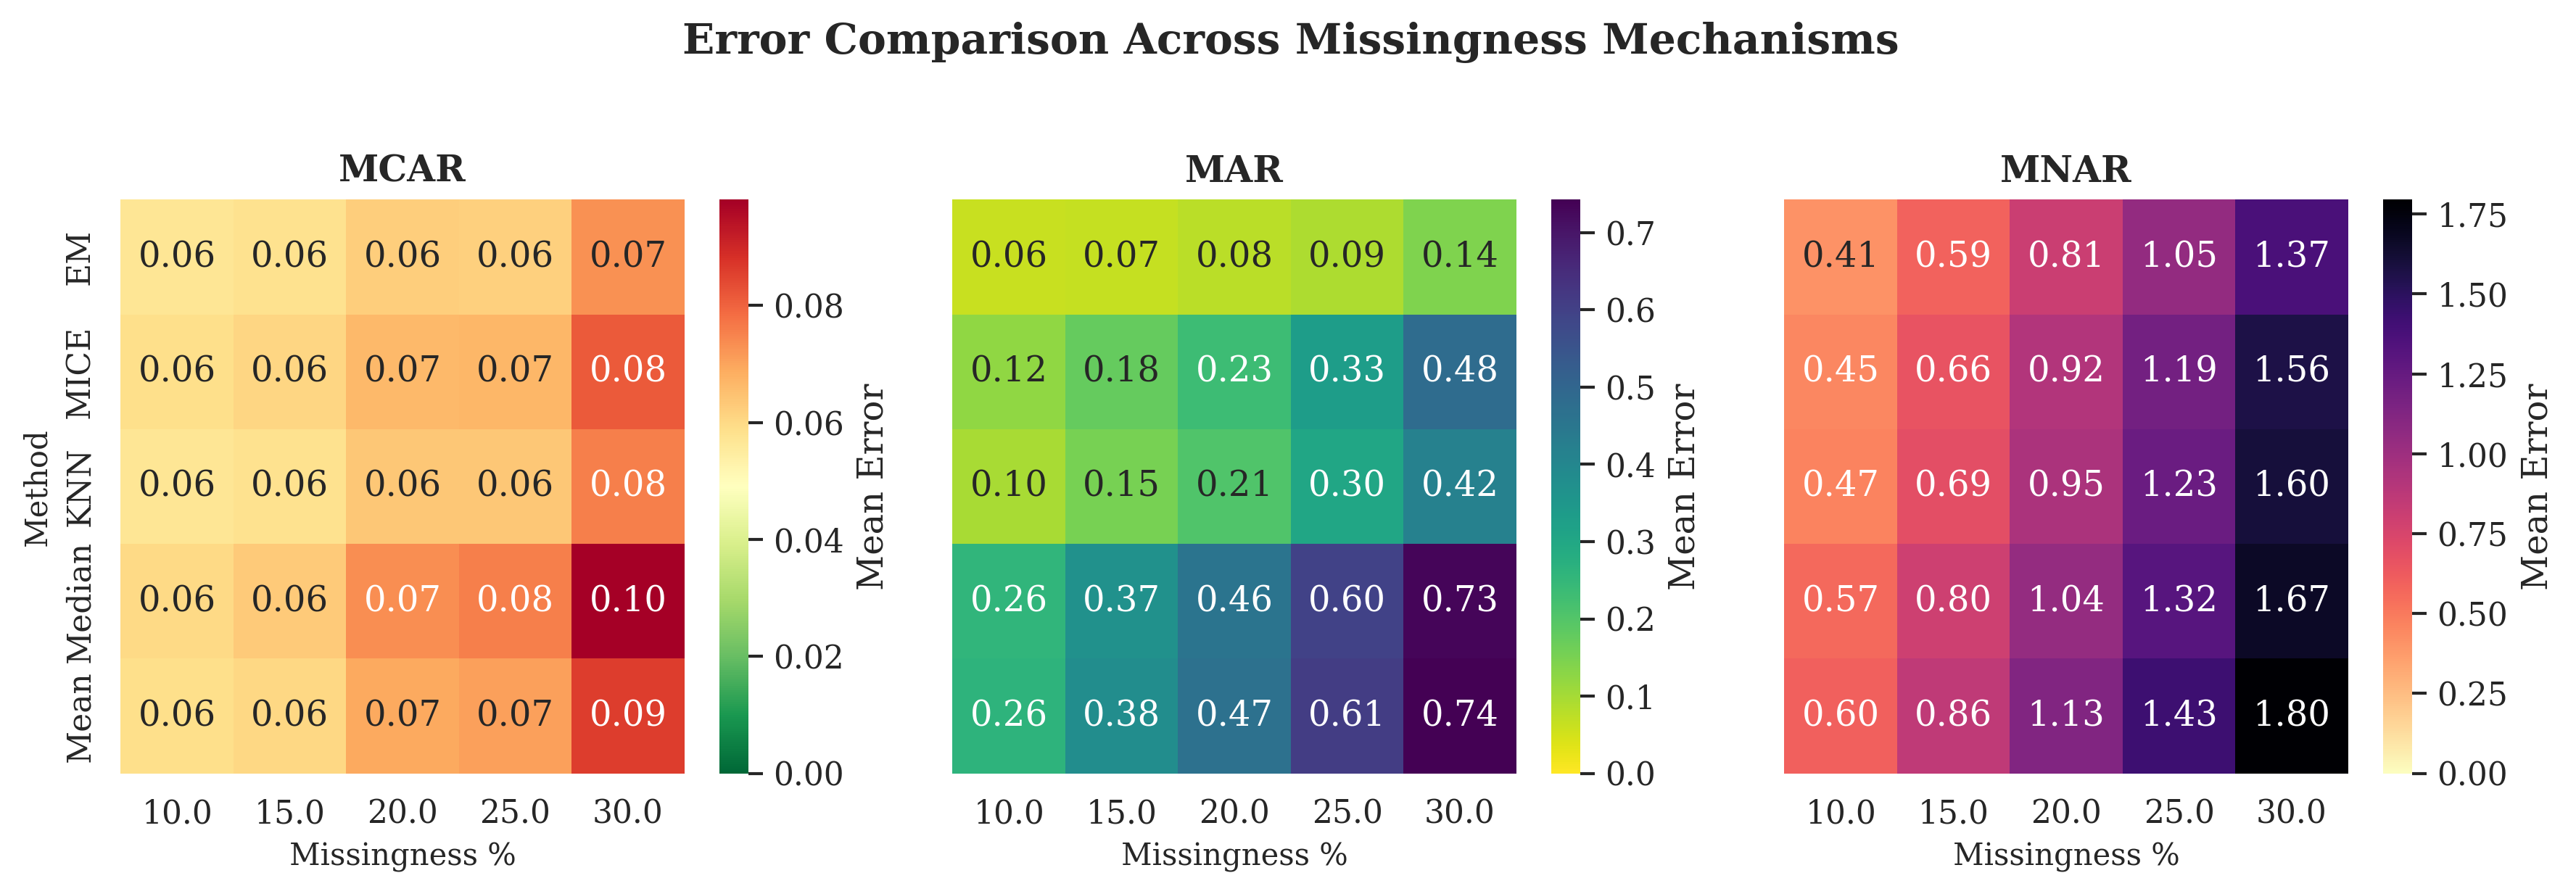
\includegraphics[width=1.0\textwidth]{plots/synthetic_multivariate/error_heatmap_all.png}
    \caption{\textbf{Mean Error Comparison Across Missingness Mechanisms.} The heatmaps display the Mean Estimation Error for varying missingness percentages (10\%--30\%), with the different imputation methods (EM, MICE, KNN, Median, Mean.).}
    \label{fig:heatmap_mvn}
\end{figure}
\paragraph{Performance Analysis.}
The heatmaps reveal distinct behavioral patterns depending on the underlying missingness mechanism:

\begin{itemize}
    \item \textbf{MCAR (Stability):} Under the Missing Completely at Random mechanism (left panel), we observe a general convergence in performance. All methods exhibit comparable results with low error rates ($\approx 0.06$). Since the missingness is independent of the data structure, even simple heuristics like Mean and Median imputation remain unbiased. Consequently, in strictly MCAR settings, the additional computational cost of complex algorithms like MICE or EM yields marginal gains.

    \item \textbf{MAR (EM Dominance):} The Missing at Random scenario (center panel) highlights the most significant performance divergence:
    \begin{itemize}
        \item The \textbf{EM algorithm} demonstrates superior robustness. It maintains the lowest error rates even as missingness increases (max error $0.14$ at $30\%$ missingness), confirming its theoretical optimality for likelihood-based inference under MAR.
        \item \textbf{kNN and MICE} perform adequately at low missingness levels ($10\%$) but exhibit a linear degradation in performance as the missingness rate increases (errors rising to $\approx 0.48$).
        \item \textbf{Mean and Median} imputation prove ineffective, with errors nearly double those of the imputation-based methods. This confirms that ignoring the observed covariates (which explain the missingness in MAR) leads to significant bias.
    \end{itemize}

    \item \textbf{MNAR (Systematic Failure):} The Missing Not at Random mechanism (right panel) results in a breakdown of all estimation strategies. The error scale increases by an order of magnitude compared to MCAR and MAR (reaching values $> 1.50$). Regardless of the method—whether parametric (EM) or non-parametric (kNN)—the bias introduced by the non-ignorable mechanism cannot be corrected without modeling the missingness process itself.
\end{itemize}

\subsubsection{The Role of Correlation Structure}
To empirically validate the EM algorithm, we analyzed the Mean Estimation Error across four distinct covariance structures. The error metrics were averaged across all sample sizes ($n$). Figure \ref{fig:correlation_grid} presents the complete comparison, highlighting a distinct structural dependency:

\begin{enumerate}
    \item \textbf{Independence (Fig. \ref{fig:cov_indep}):} Under zero correlation ($\Sigma = \mathbf{I}$), univariate baselines (Mean, Median) outperform multivariate methods (EM, MICE), which tend to overfit by modeling non-existent relationships.
    
    \item \textbf{Correlated Structures (Figs. \ref{fig:cov_weak}--\ref{fig:cov_block}):} As correlation increases, the hierarchy inverts. EM dominates by leveraging dependencies (whether global or local) to minimize error, while univariate methods fail to capture the data structure, resulting in significant bias.
\end{enumerate}

\begin{figure}[H]
    \centering
    % Riga 1
    \begin{subfigure}[b]{0.48\textwidth}
        \centering
        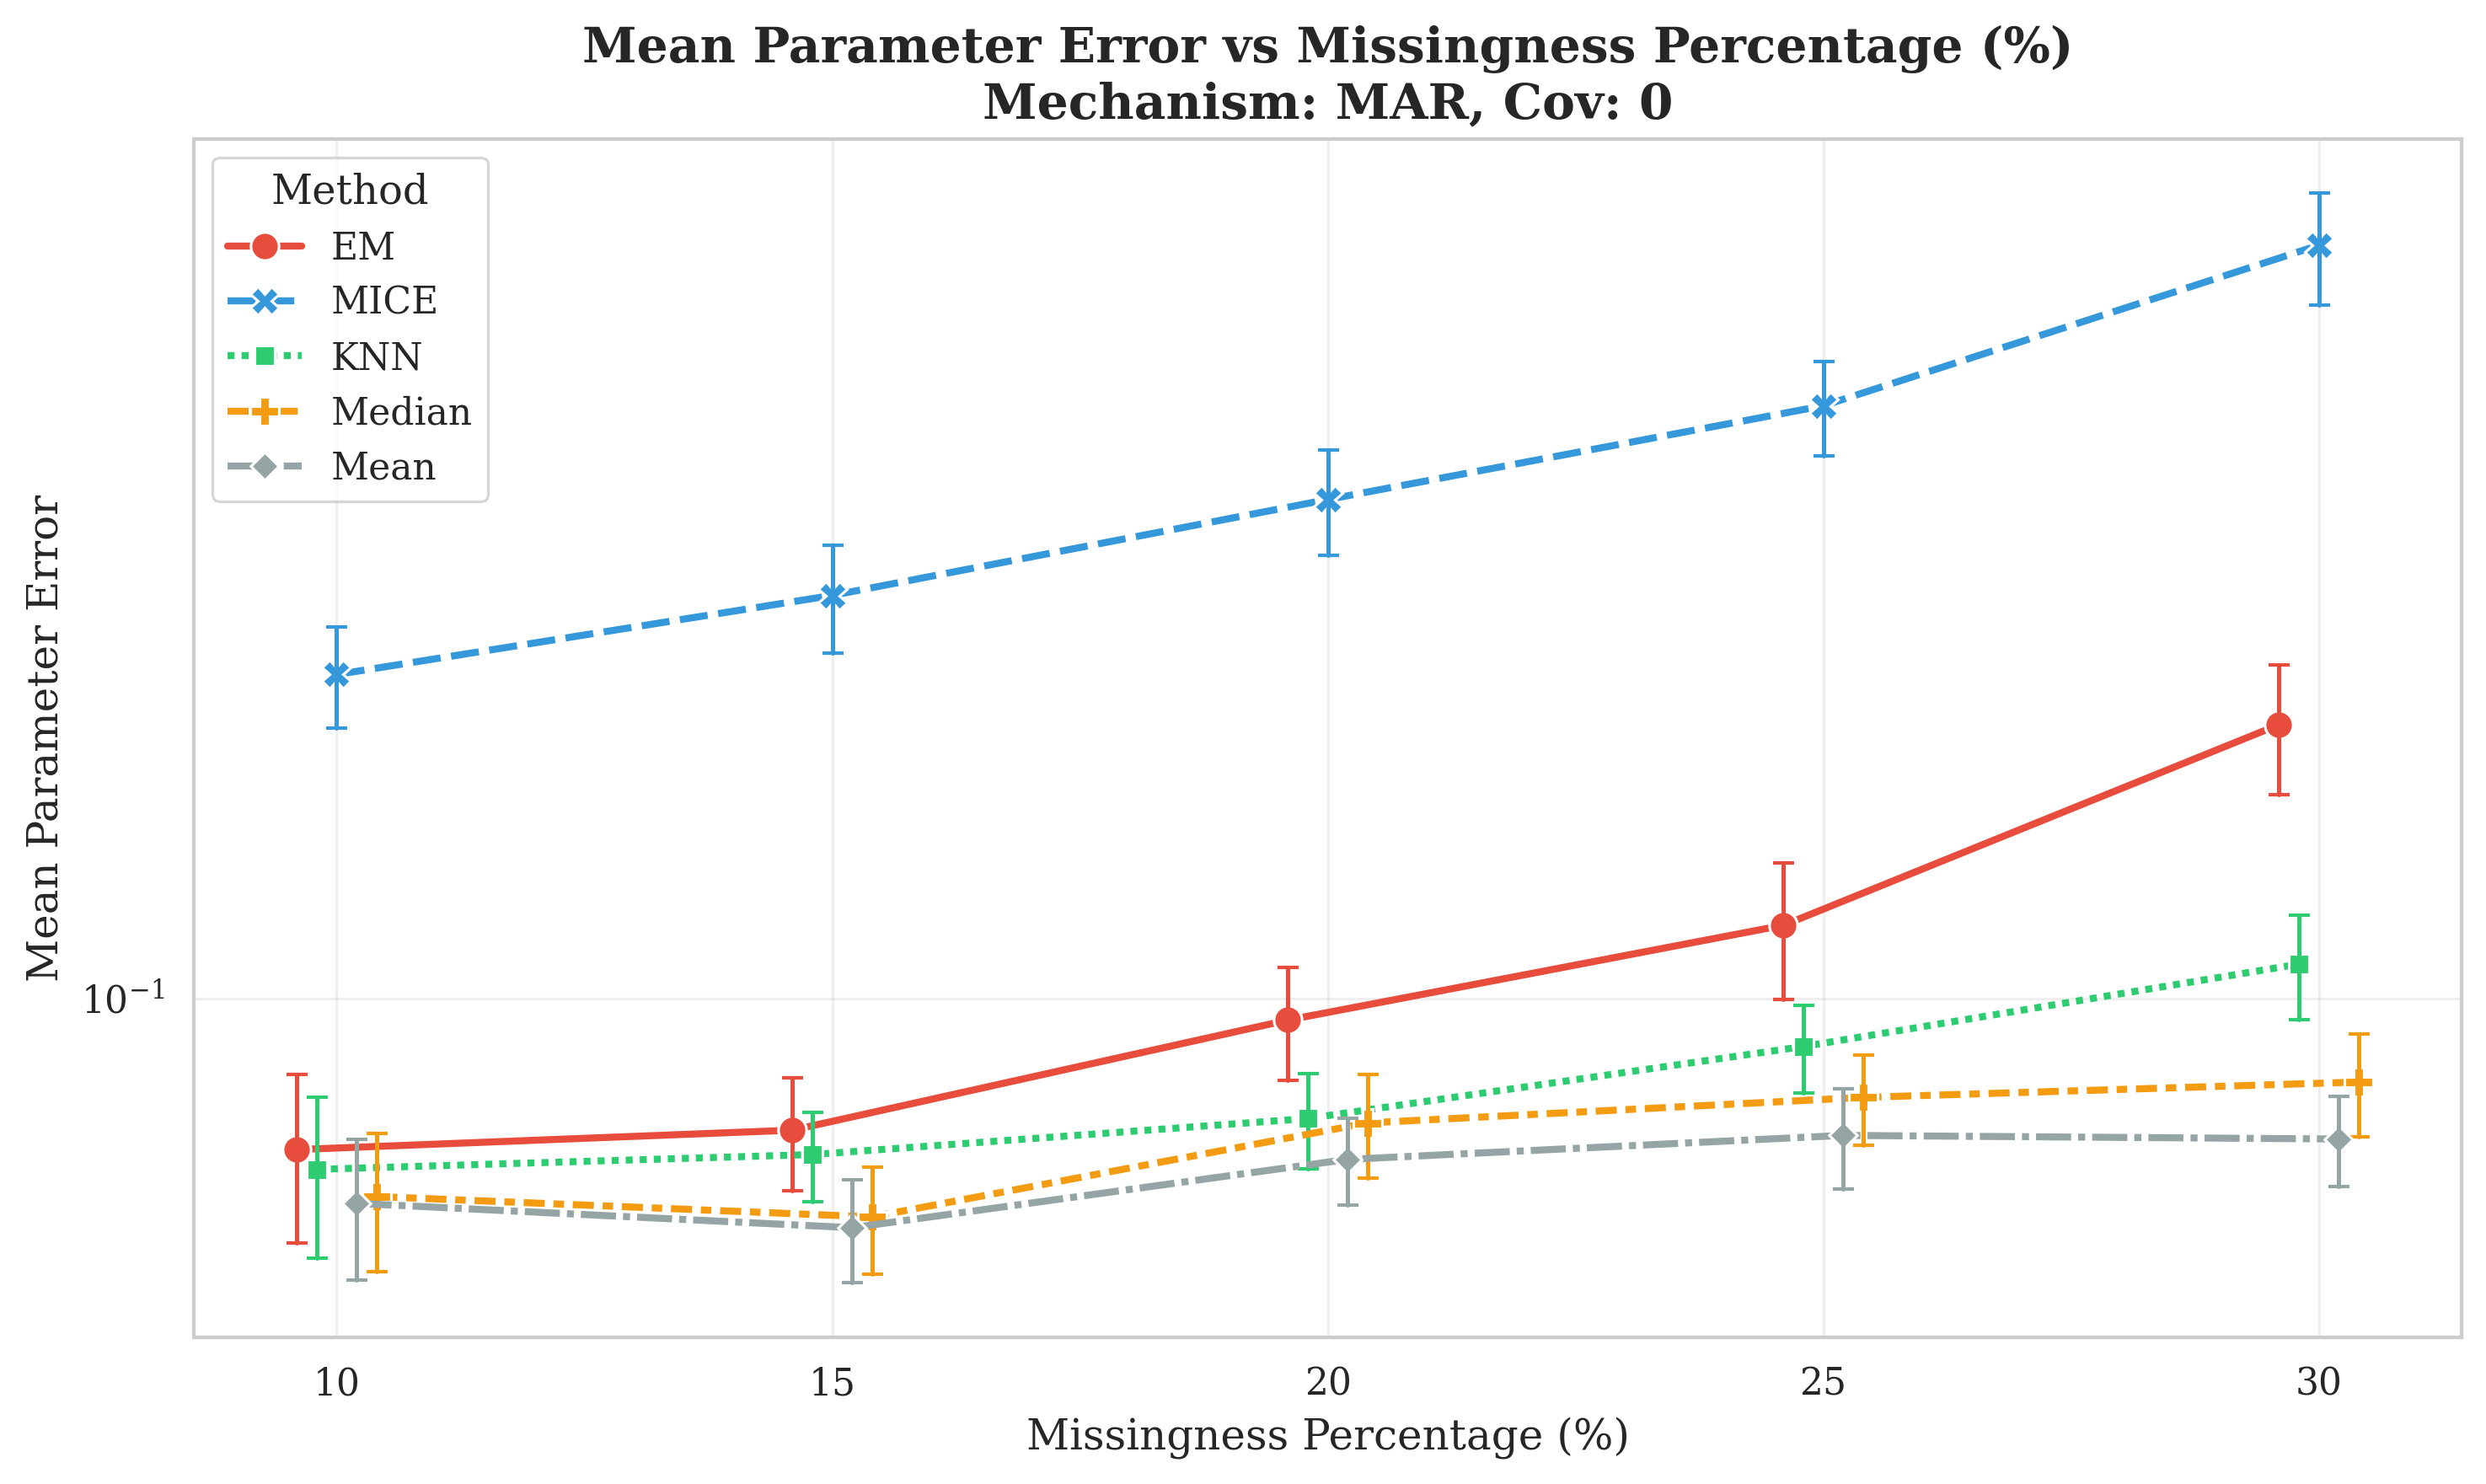
\includegraphics[width=\textwidth]{plots/additional_visualizations/mvn_covariance_structures/MAR_Indep_error.png}
        \caption{\textbf{Independence ($\Sigma = \mathbf{I}$)}.}
        \label{fig:cov_indep}
    \end{subfigure}
    \hfill
    \begin{subfigure}[b]{0.48\textwidth}
        \centering
        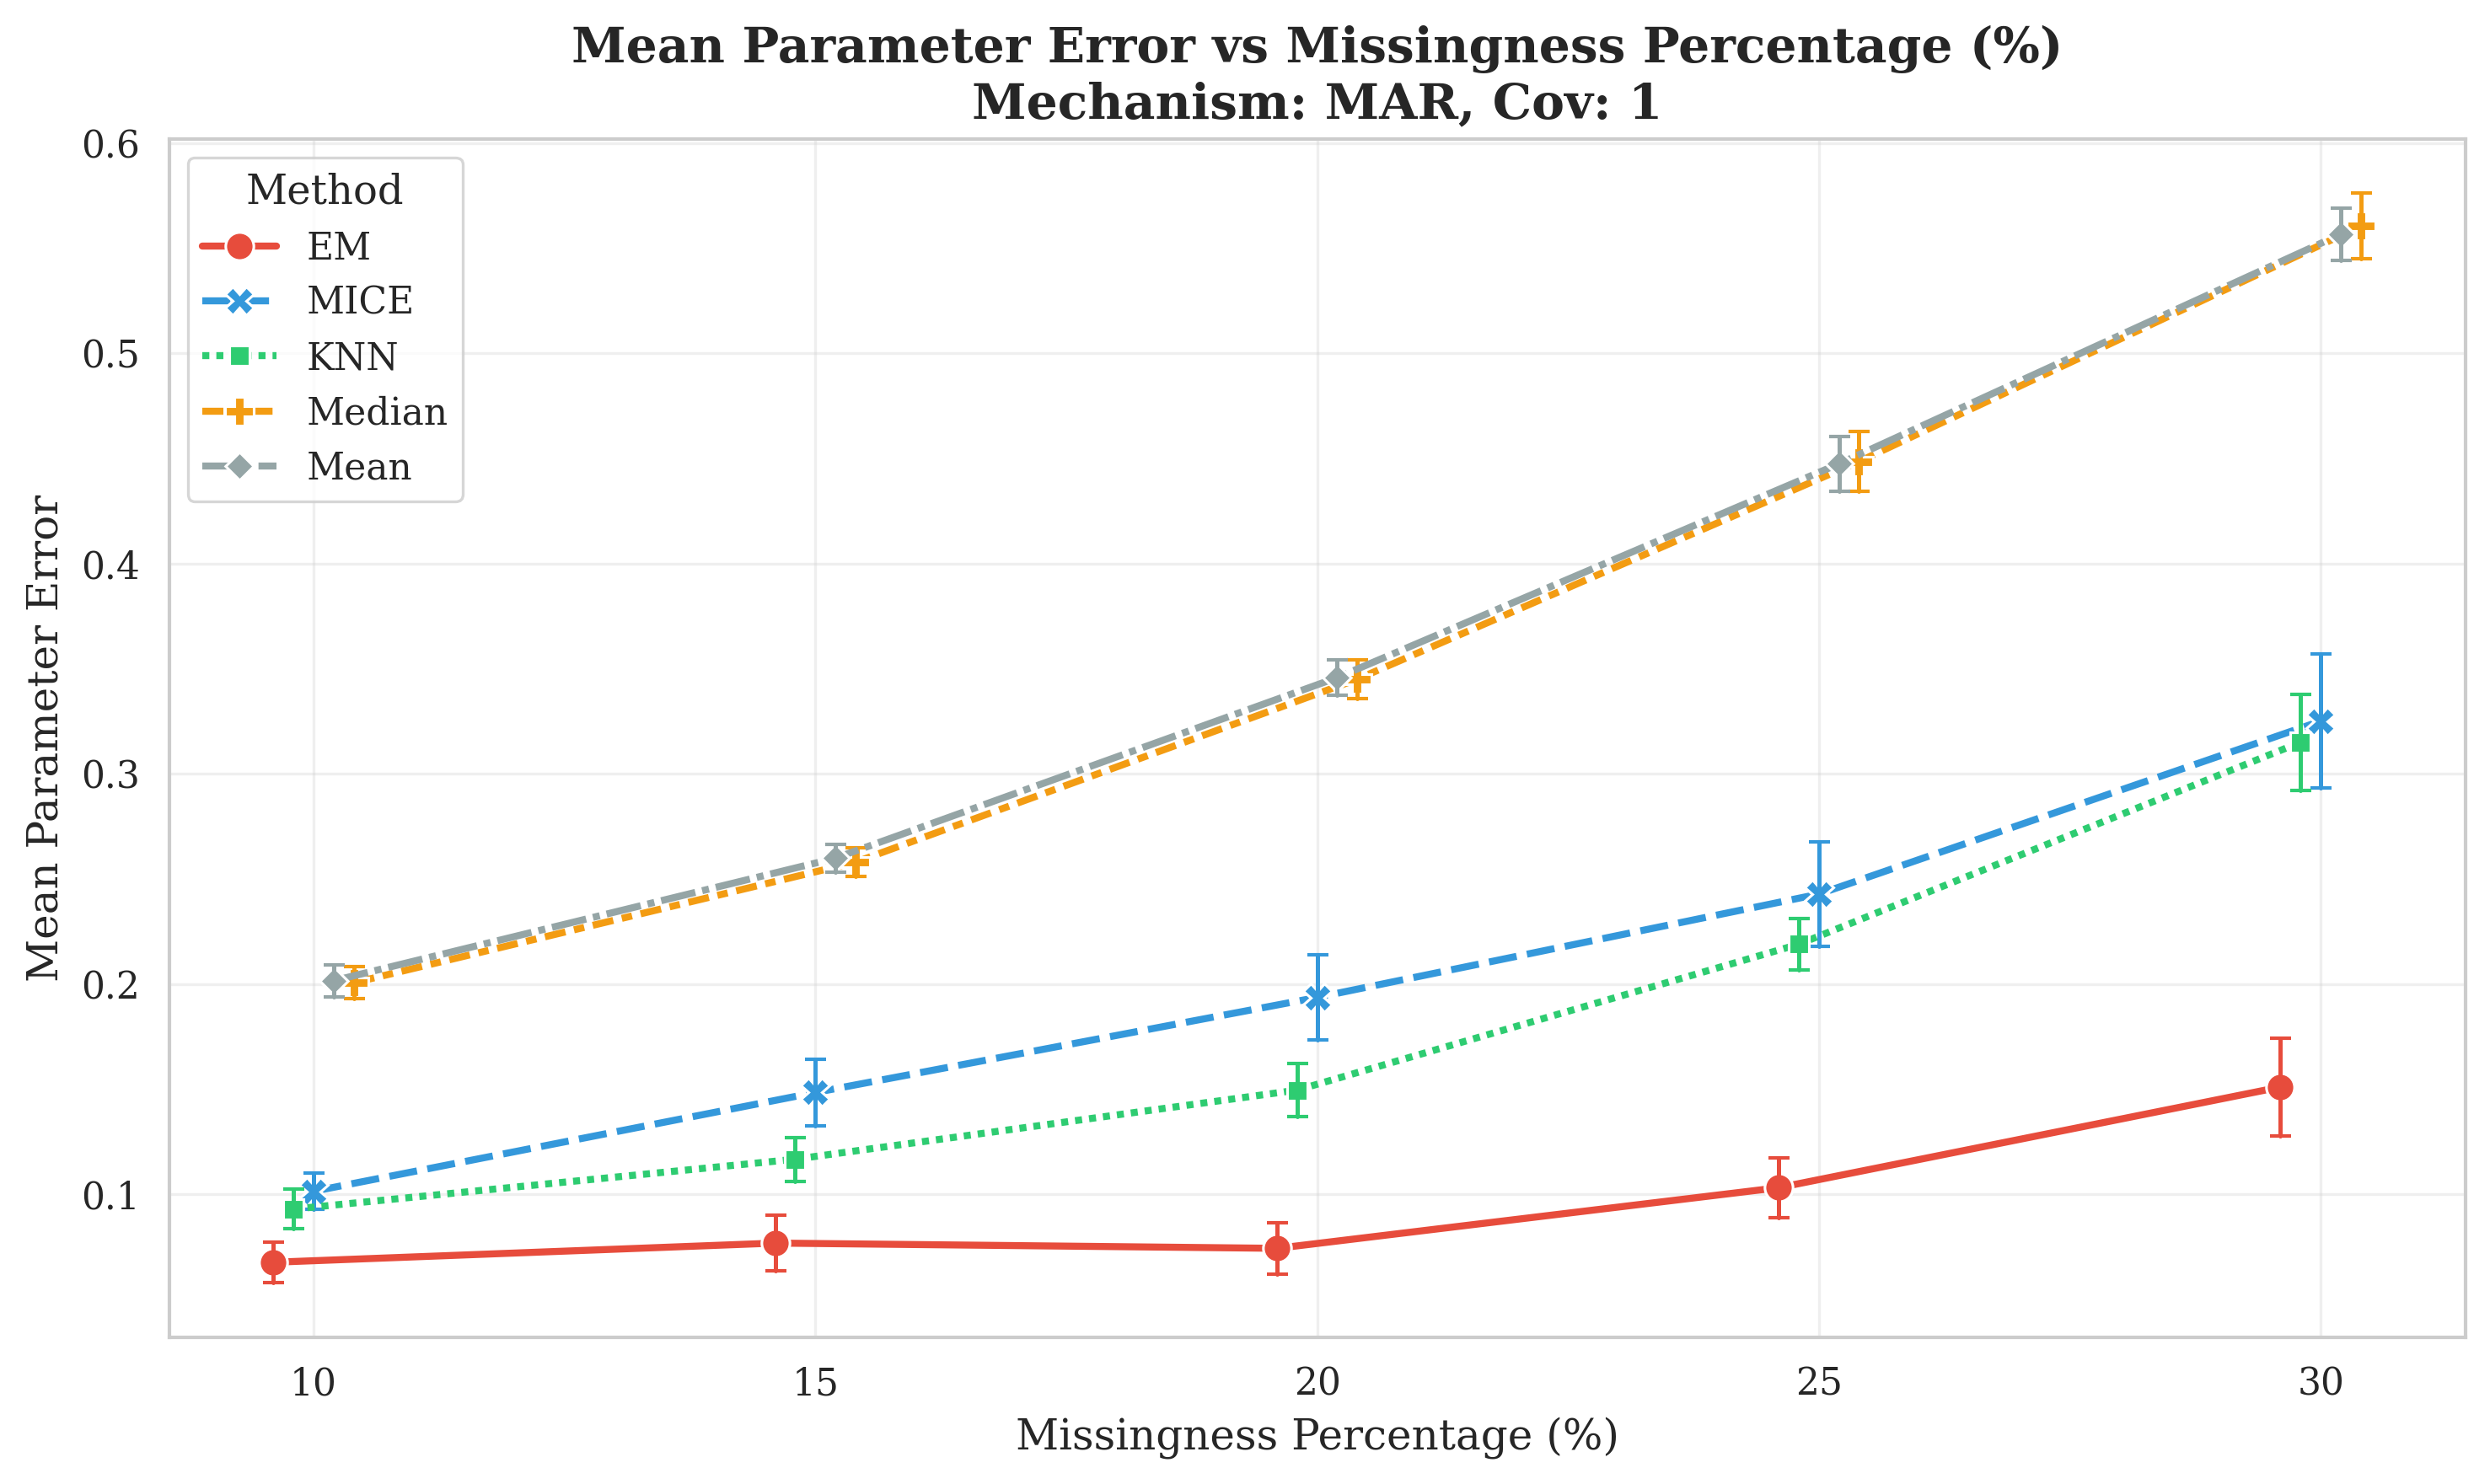
\includegraphics[width=\textwidth]{plots/additional_visualizations/mvn_covariance_structures/MAR_Weak_error.png}
        \caption{\textbf{Weak Correlation ($\rho=0.3$).}}
        \label{fig:cov_weak}
    \end{subfigure}
    
    \vspace{1em} % Spazio verticale
    
    % Riga 2
    \begin{subfigure}[b]{0.48\textwidth}
        \centering
        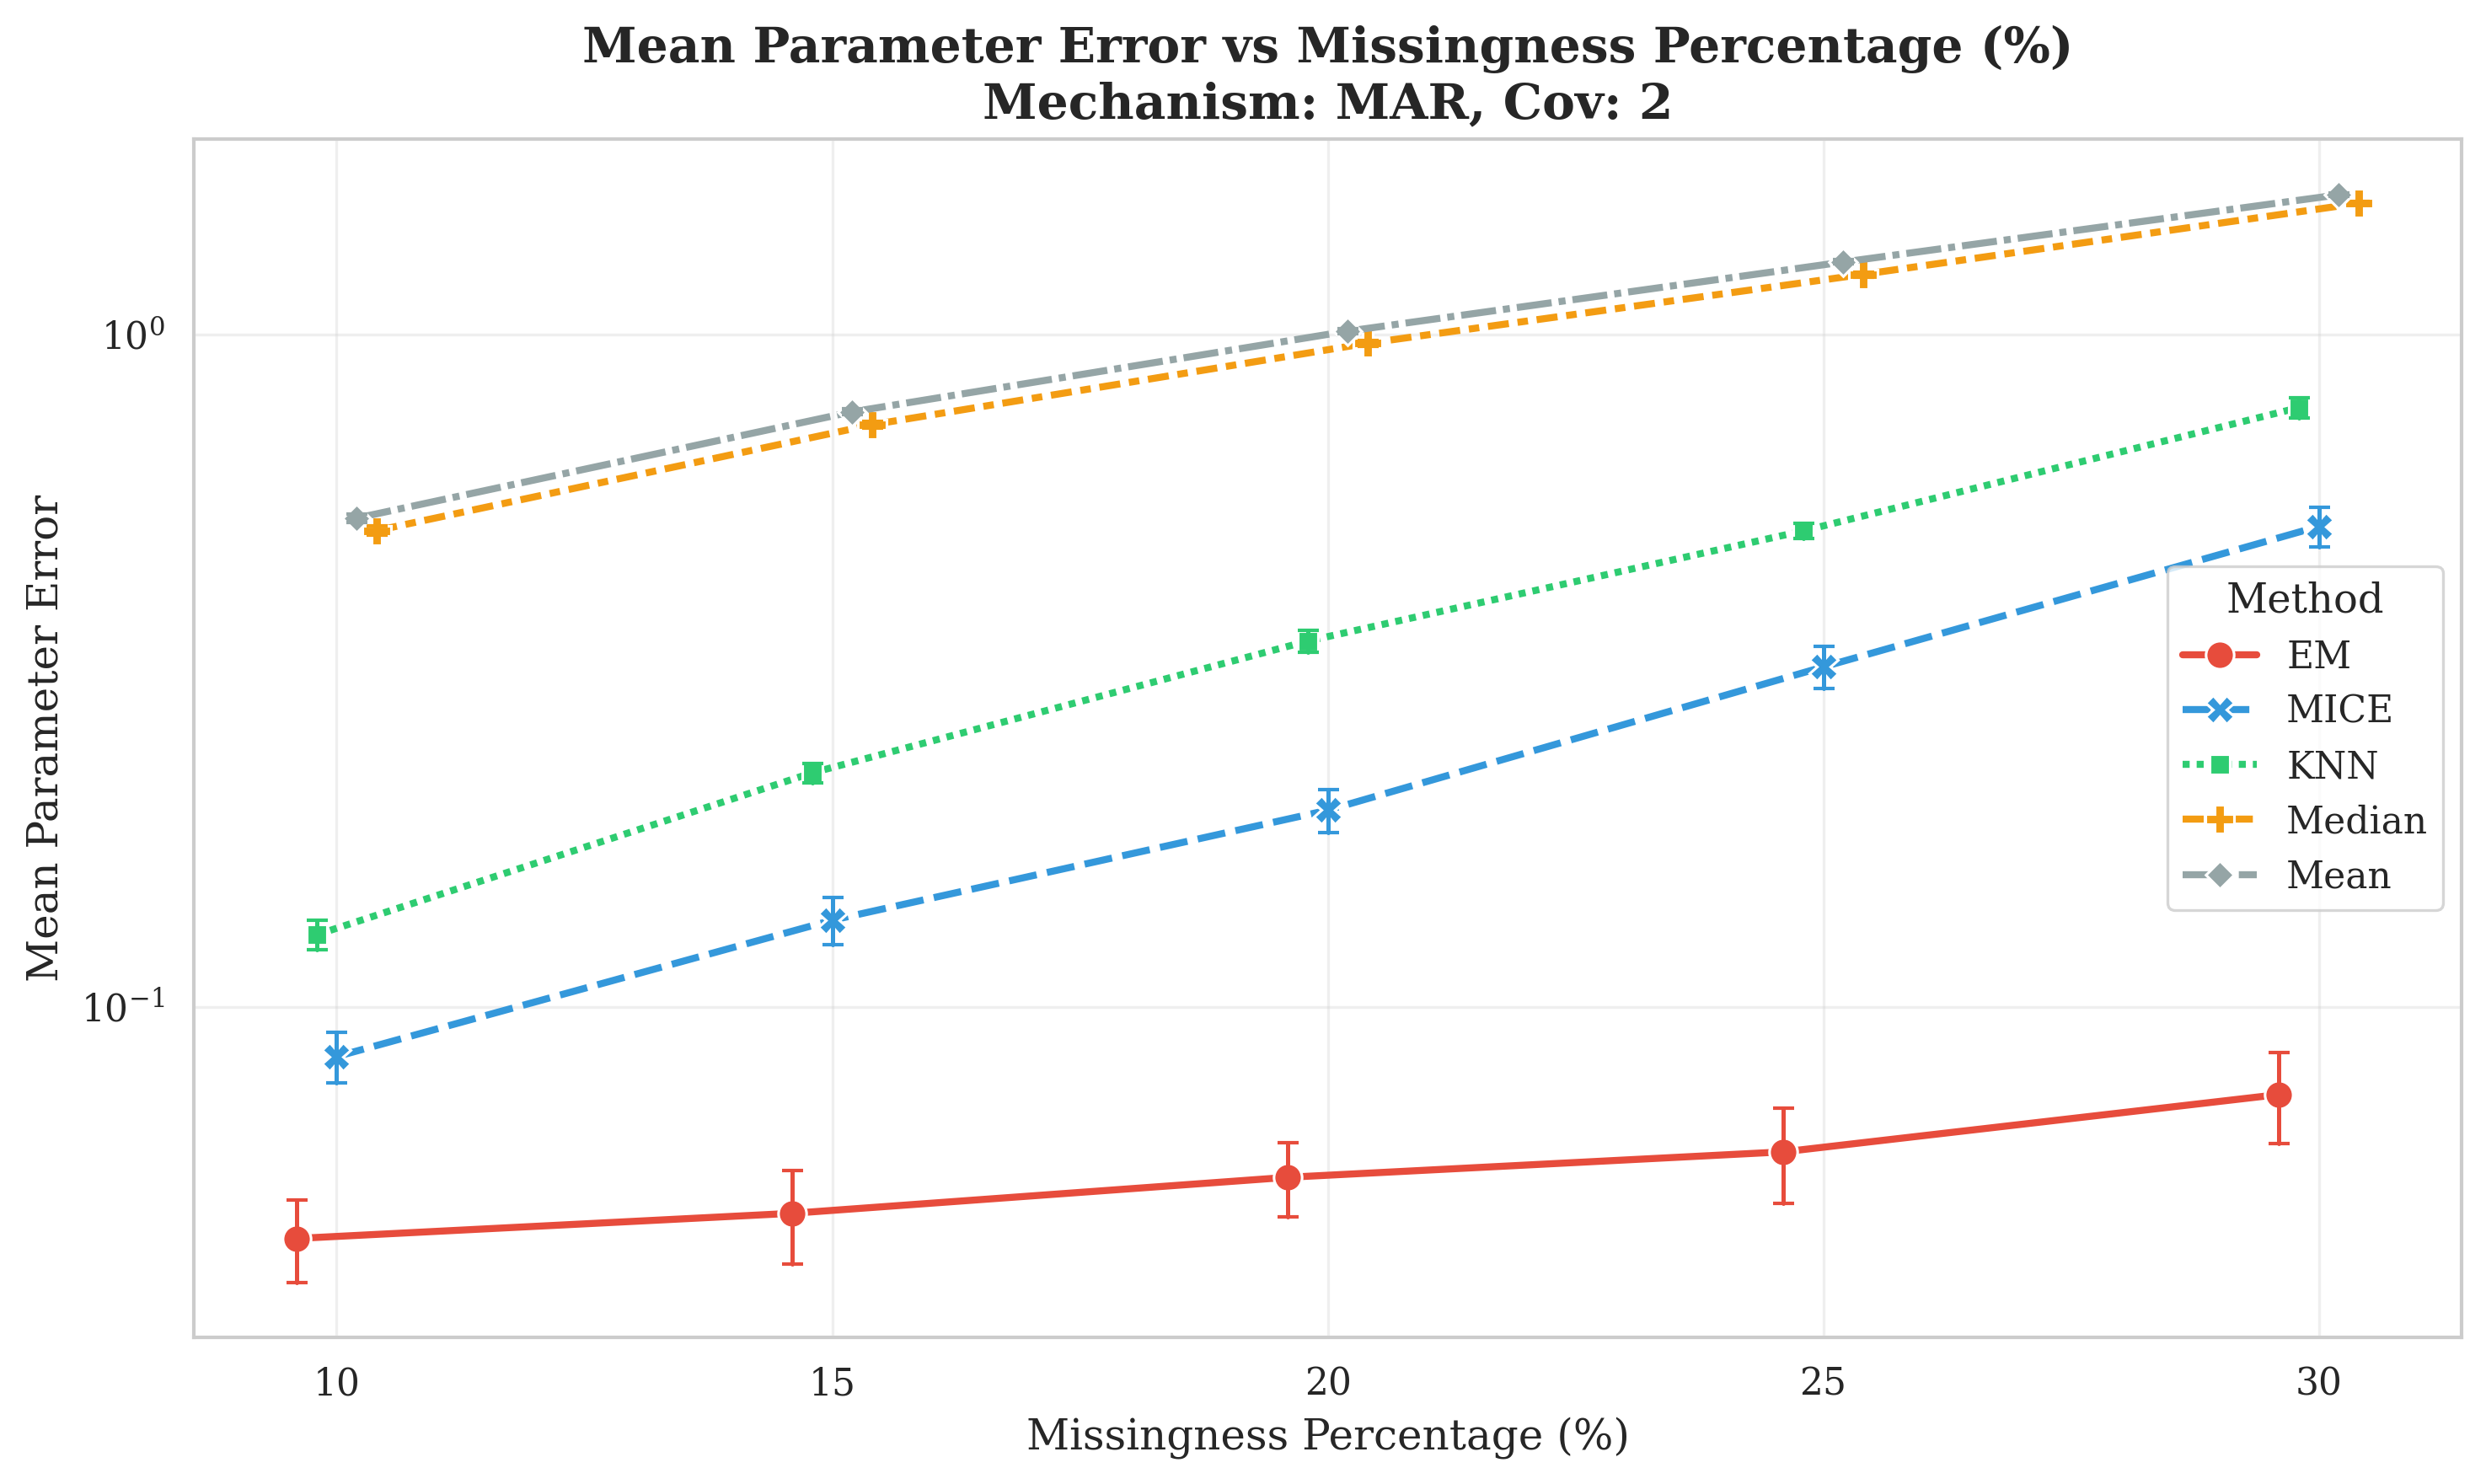
\includegraphics[width=\textwidth]{plots/additional_visualizations/mvn_covariance_structures/MAR_Strong_error.png}
        \caption{\textbf{Strong Correlation ($\rho=0.9$).}}
        \label{fig:cov_strong}
    \end{subfigure}
    \hfill
    \begin{subfigure}[b]{0.48\textwidth}
        \centering
        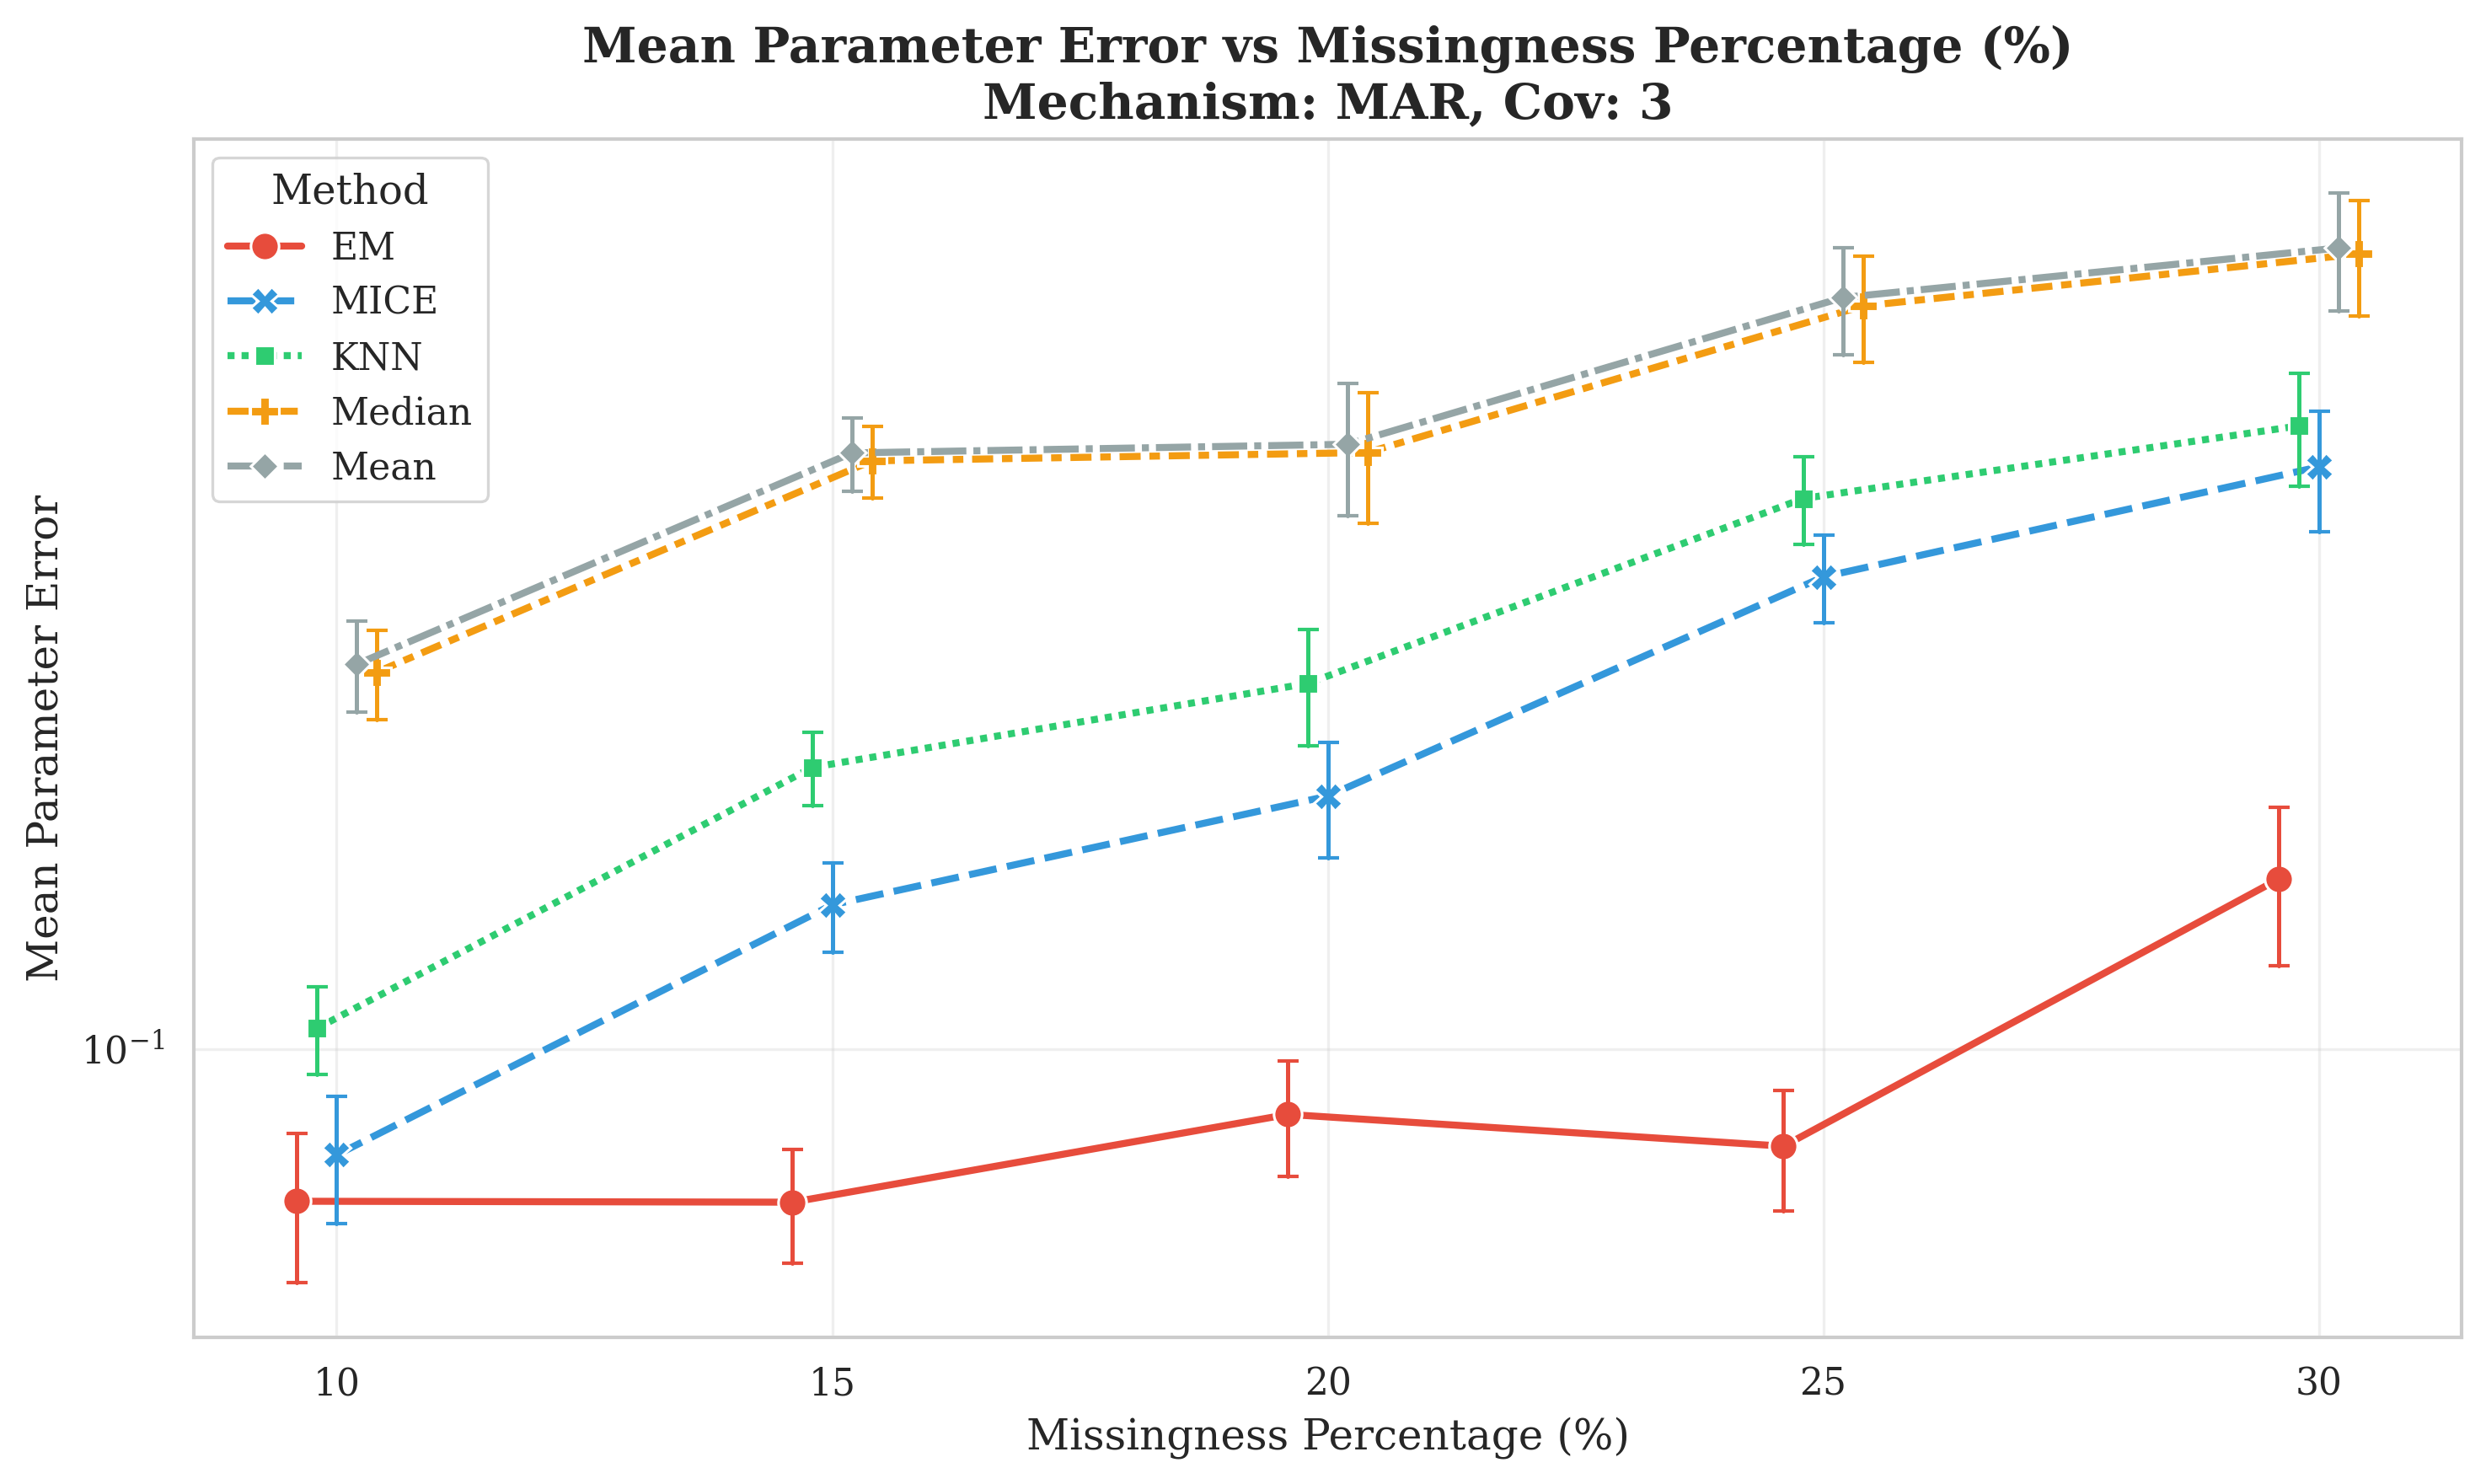
\includegraphics[width=\textwidth]{plots/additional_visualizations/mvn_covariance_structures/MAR_Block_error.png}
        \caption{\textbf{Block Correlation.}}
        \label{fig:cov_block}
    \end{subfigure}
    
    \caption{\textbf{Mean Estimation Error under MAR.} Performance comparison across covariance settings.}
    \label{fig:correlation_grid}
\end{figure}
Furthermore, while univariate methods like Mean Imputation appear competitive for estimating location parameters ($\boldsymbol{\mu}$) under independence, they fail catastrophically at preserving the data's variability and shape ($\boldsymbol{\Sigma}$). Figure \ref{fig:covariance_analysis} highlights this crucial trade-off.

\begin{figure}[H]
    \centering
    % Plot 1: Independence Covariance 
    % PROOF: Mean Imputation destroys variance (grey line goes up)
    \begin{subfigure}[b]{0.48\textwidth}
        \centering
        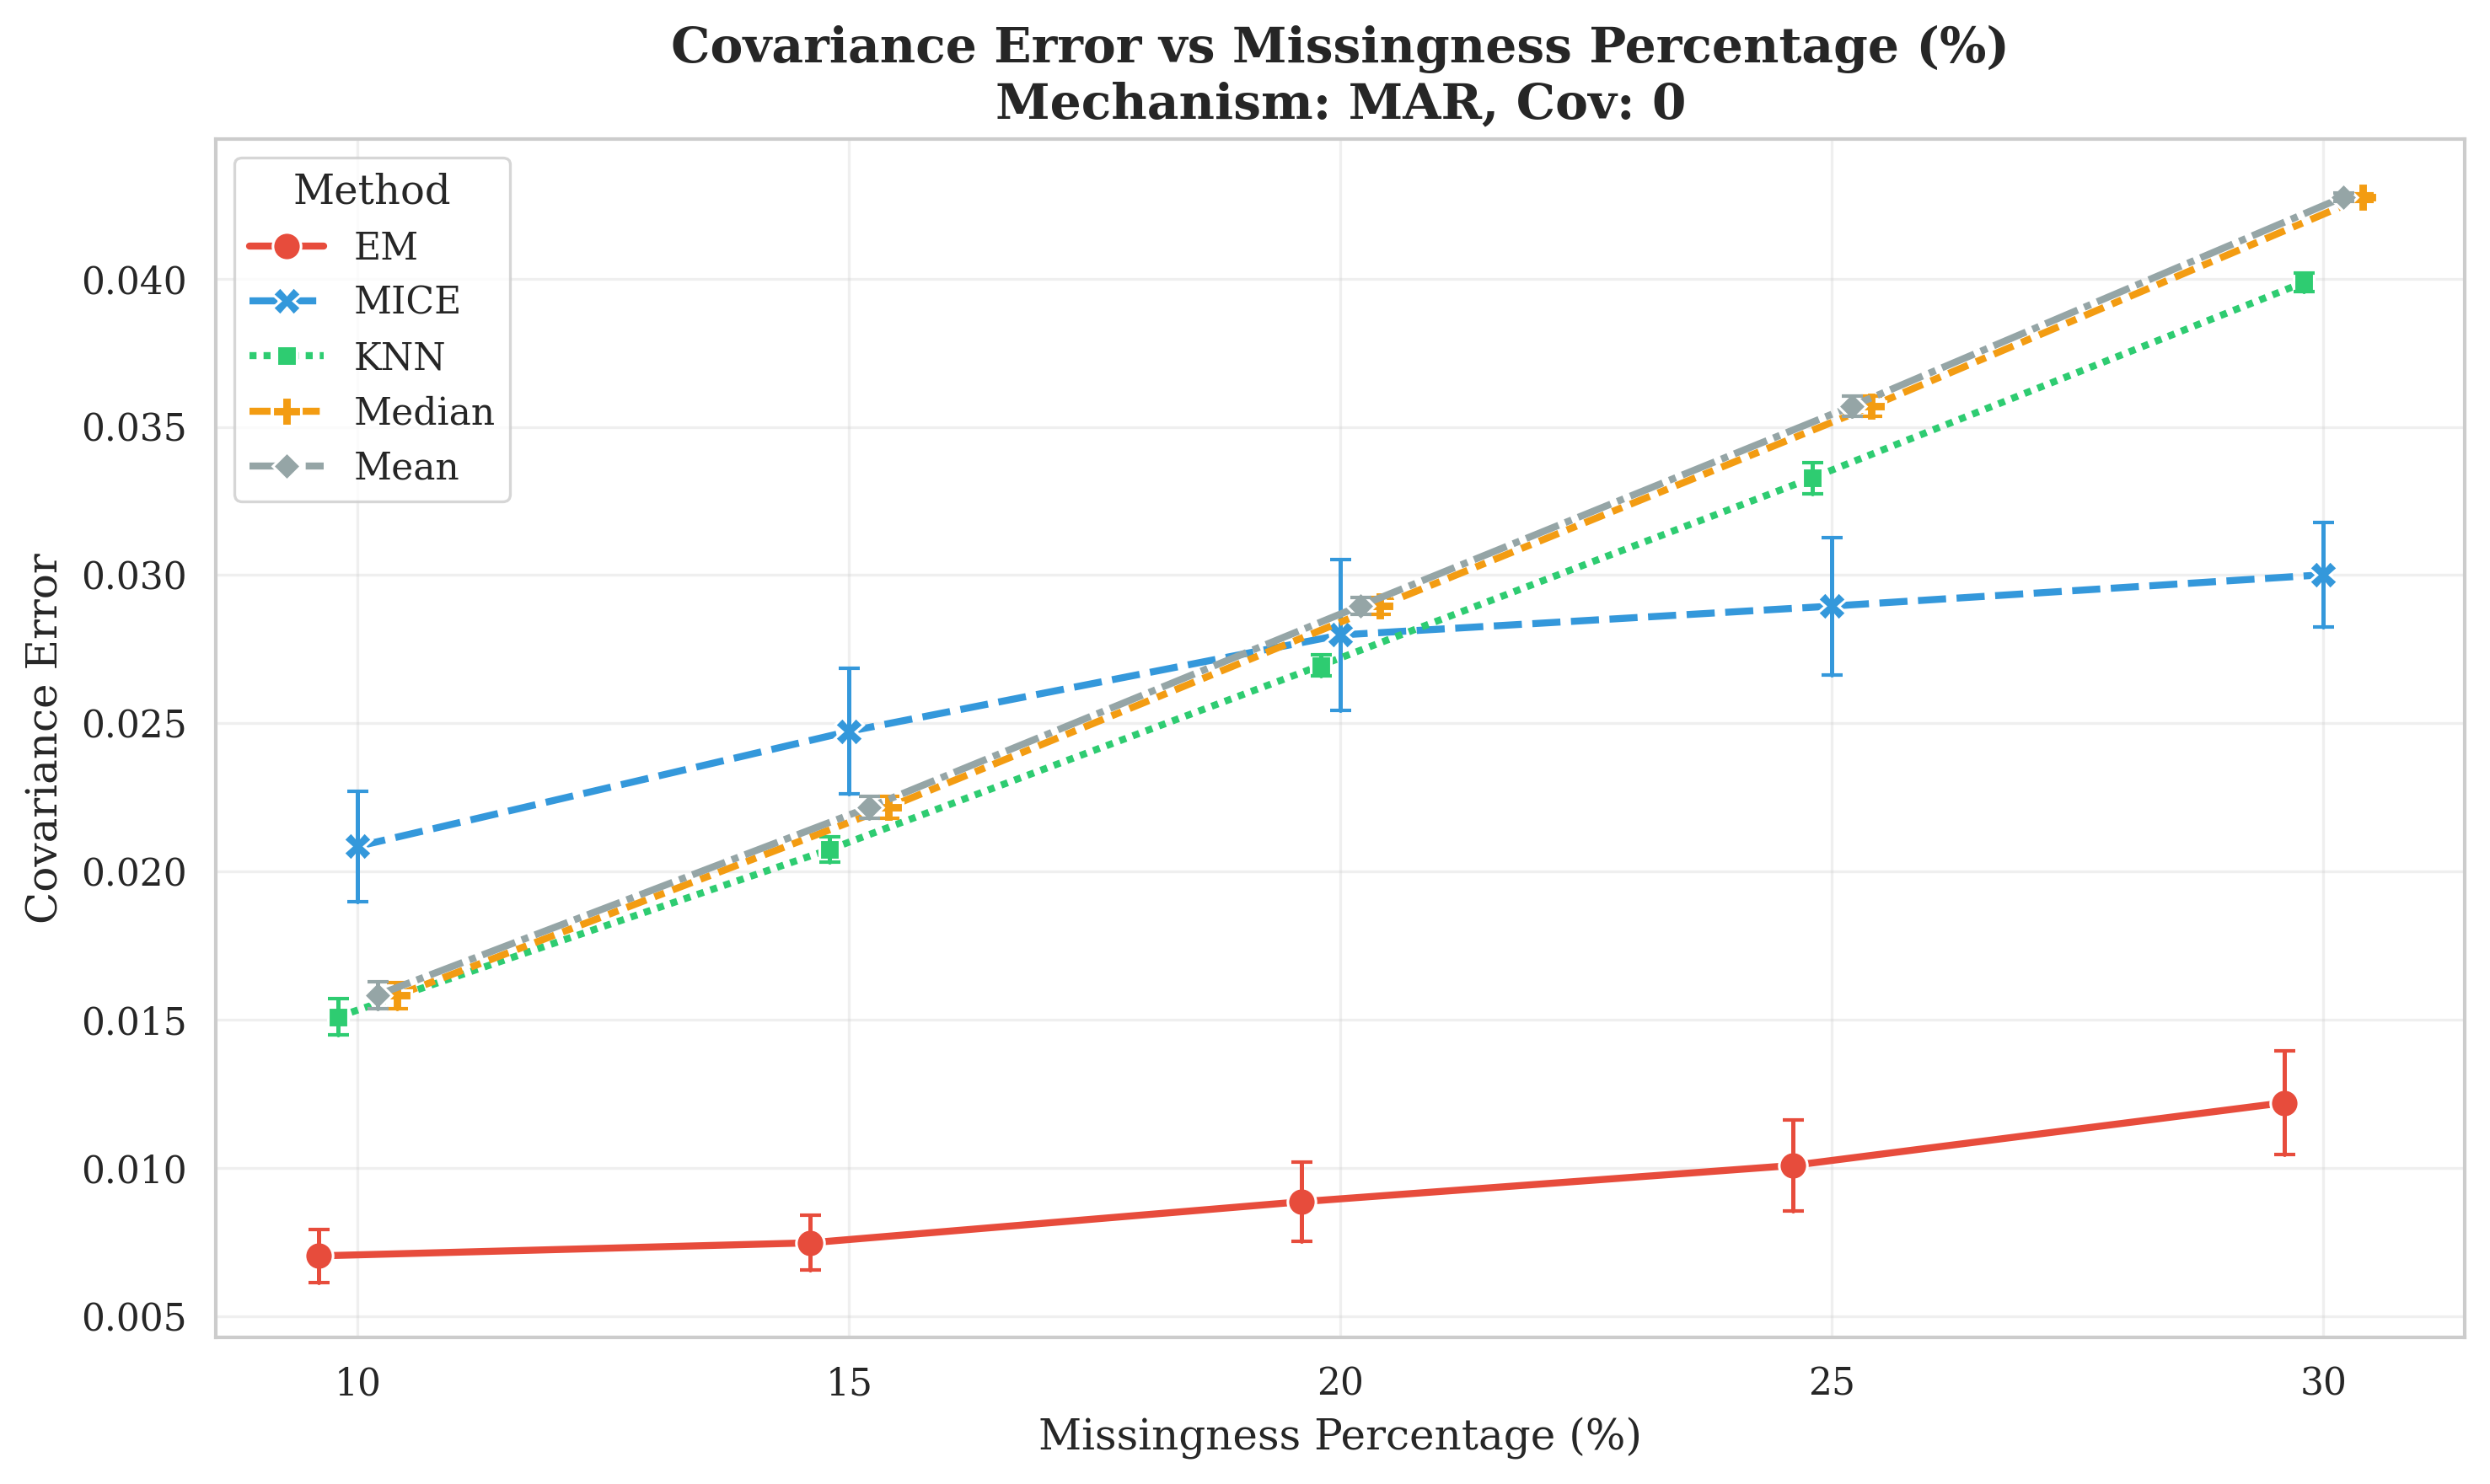
\includegraphics[width=\textwidth]{plots/additional_visualizations/mvn_covariance_structures/MAR_Indep_cov_error.png}
        \caption{Covariance Error. Mechanism: MAR. Stuctural Case: \textbf{Independence ($\Sigma = \mathbf{I}$).}}
        \label{fig:cov_error_indep}
    \end{subfigure}
    \hfill
    % Plot 2: Block Covariance
    % PROOF: EM correctly identifies complex structures
    \begin{subfigure}[b]{0.48\textwidth}
        \centering
        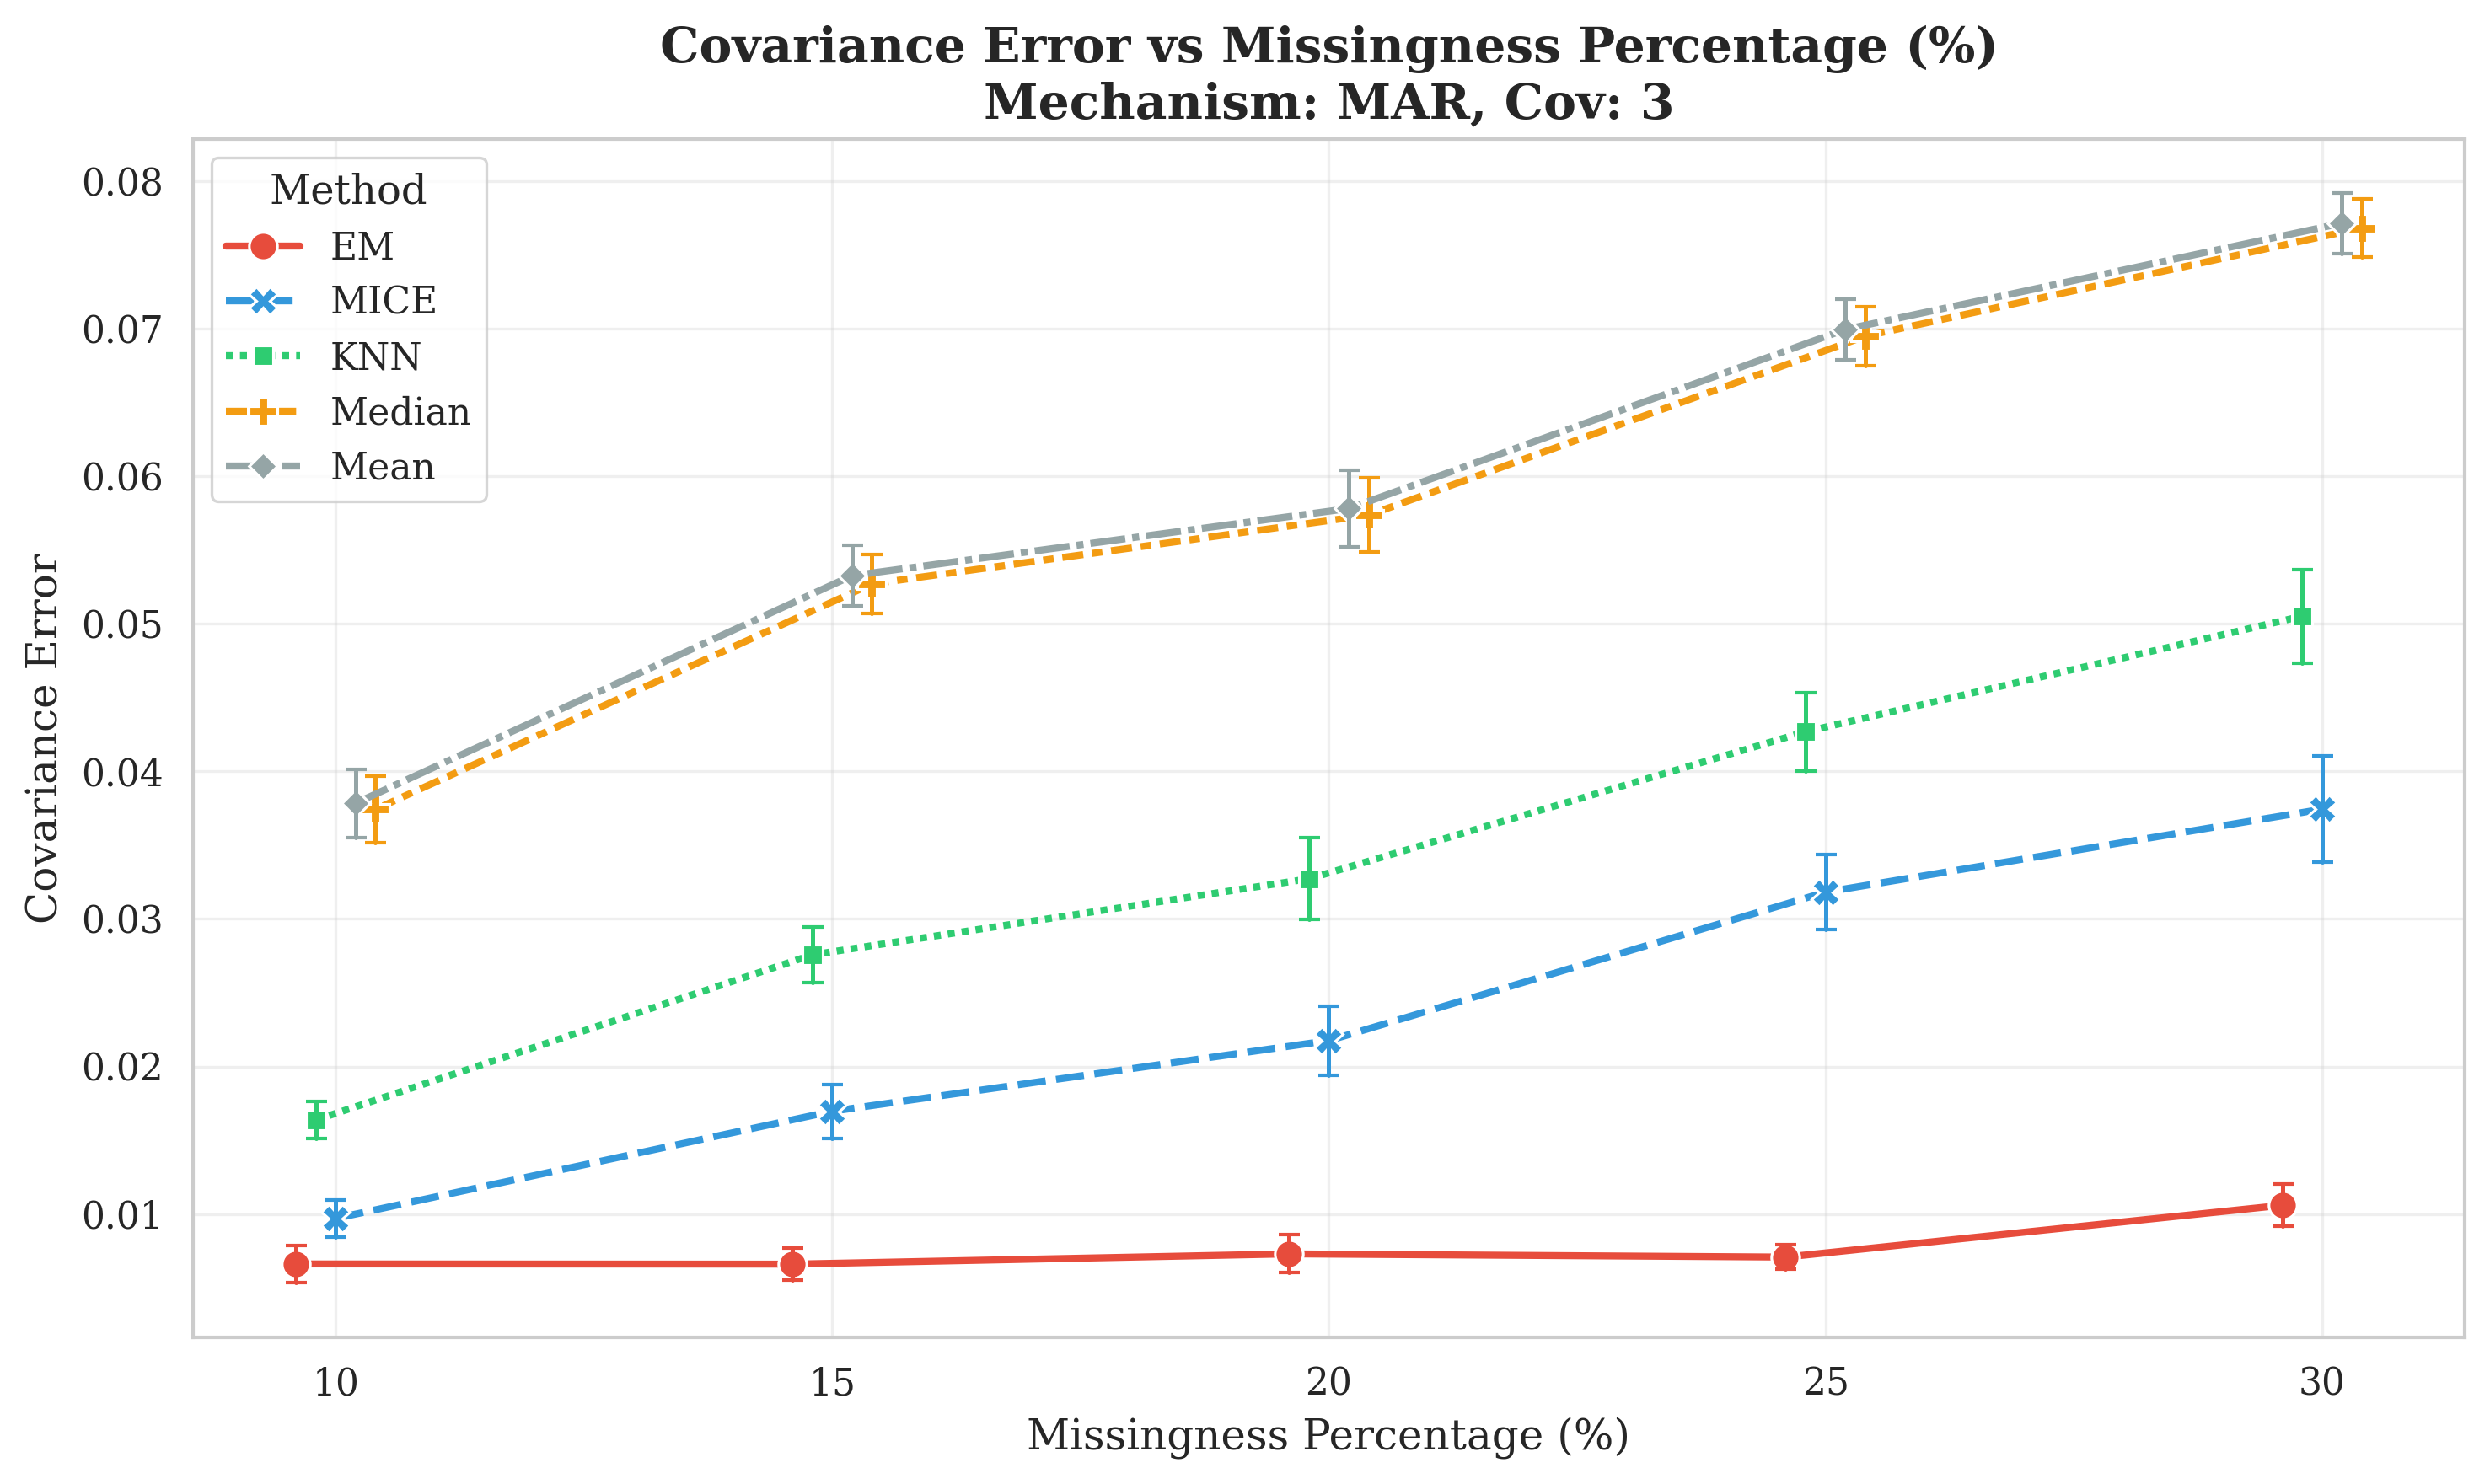
\includegraphics[width=\textwidth]{plots/additional_visualizations/mvn_covariance_structures/MAR_Block_cov_error.png}
        \caption{Mean Error. Mechanism: MAR. Stuctural Case: \textbf{Block Correlation.}}
        \label{fig:cov_error_block}
    \end{subfigure}
    
    \caption{\textbf{Covariance Estimation Error under MAR.} Performance comparison across Independence and Block Correlation.}
    \label{fig:covariance_analysis}
\end{figure}
Unlike in mean estimation (Fig. \ref{fig:correlation_grid}), here EM dominates across all scenarios. In panel (a), Mean Imputation's error increases linearly with missingness. Replacing missing values with a constant systematically underestimates the sample variance.

\subsubsection{Sensitivity to MNAR Mechanism}
We evaluated the robustness of the algorithms when the missingness mechanism is non-ignorable (MNAR). Figure \ref{fig:mnar_failure} compares the performance under Strong Correlation for the MNAR case.

\begin{figure}[H]
    \centering
    % MNAR Plot: Shows that error does not go to zero
    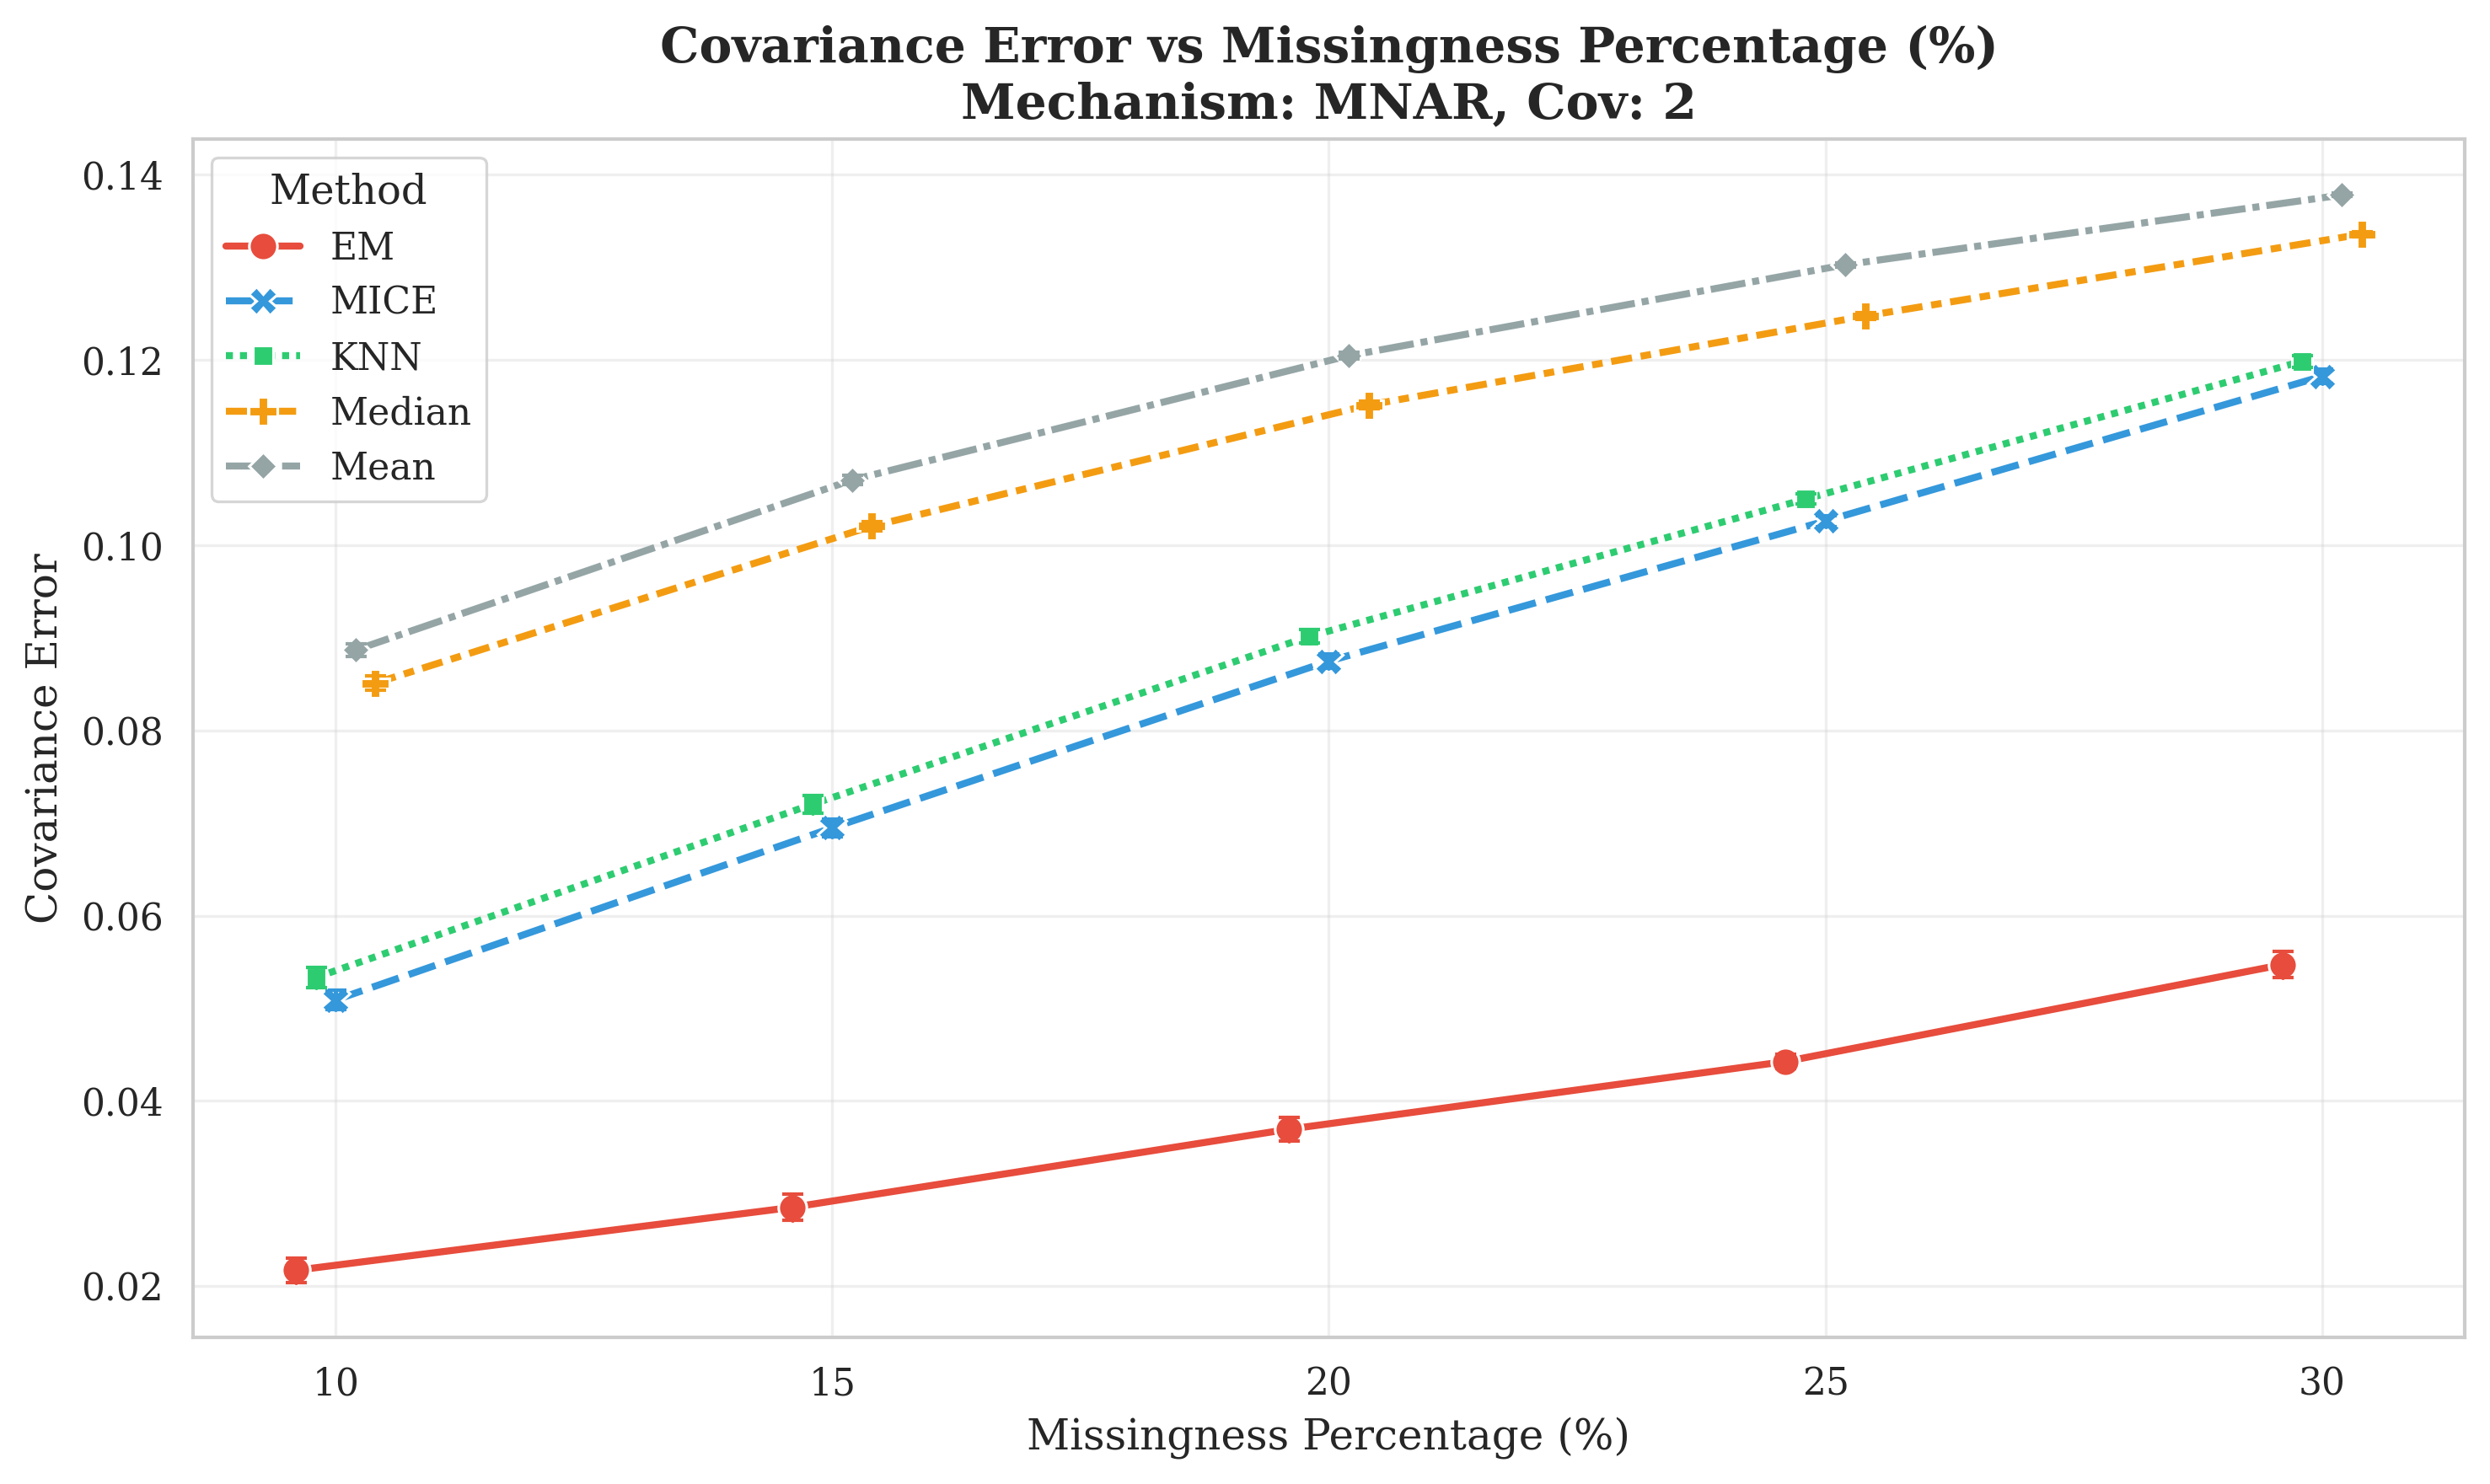
\includegraphics[width=0.7\textwidth]{plots/additional_visualizations/mvn_covariance_structures/MNAR_Strong_cov_error.png}
    \caption{\textbf{Mean Estimation Error under MNAR.} Note the vertical scale shift compared to MAR. Even the EM algorithm (red) incurs a persistent bias that does not vanish, confirming that likelihood maximization cannot correct for self-censorship without explicit modeling of the missingness mechanism.}
    \label{fig:mnar_failure}
\end{figure}

\paragraph{Asymptotic Bias under MNAR}
Can ``Big Data'' solve the missing data problem? We analyzed the asymptotic behavior of the error as the sample size $n$ increases under the MNAR mechanism. Unlike the previous analyses, the error reported here is computed by fixing the sample size and averaging across all varying missingness percentages and covariance structures.

\begin{figure}[h!]
    \centering
    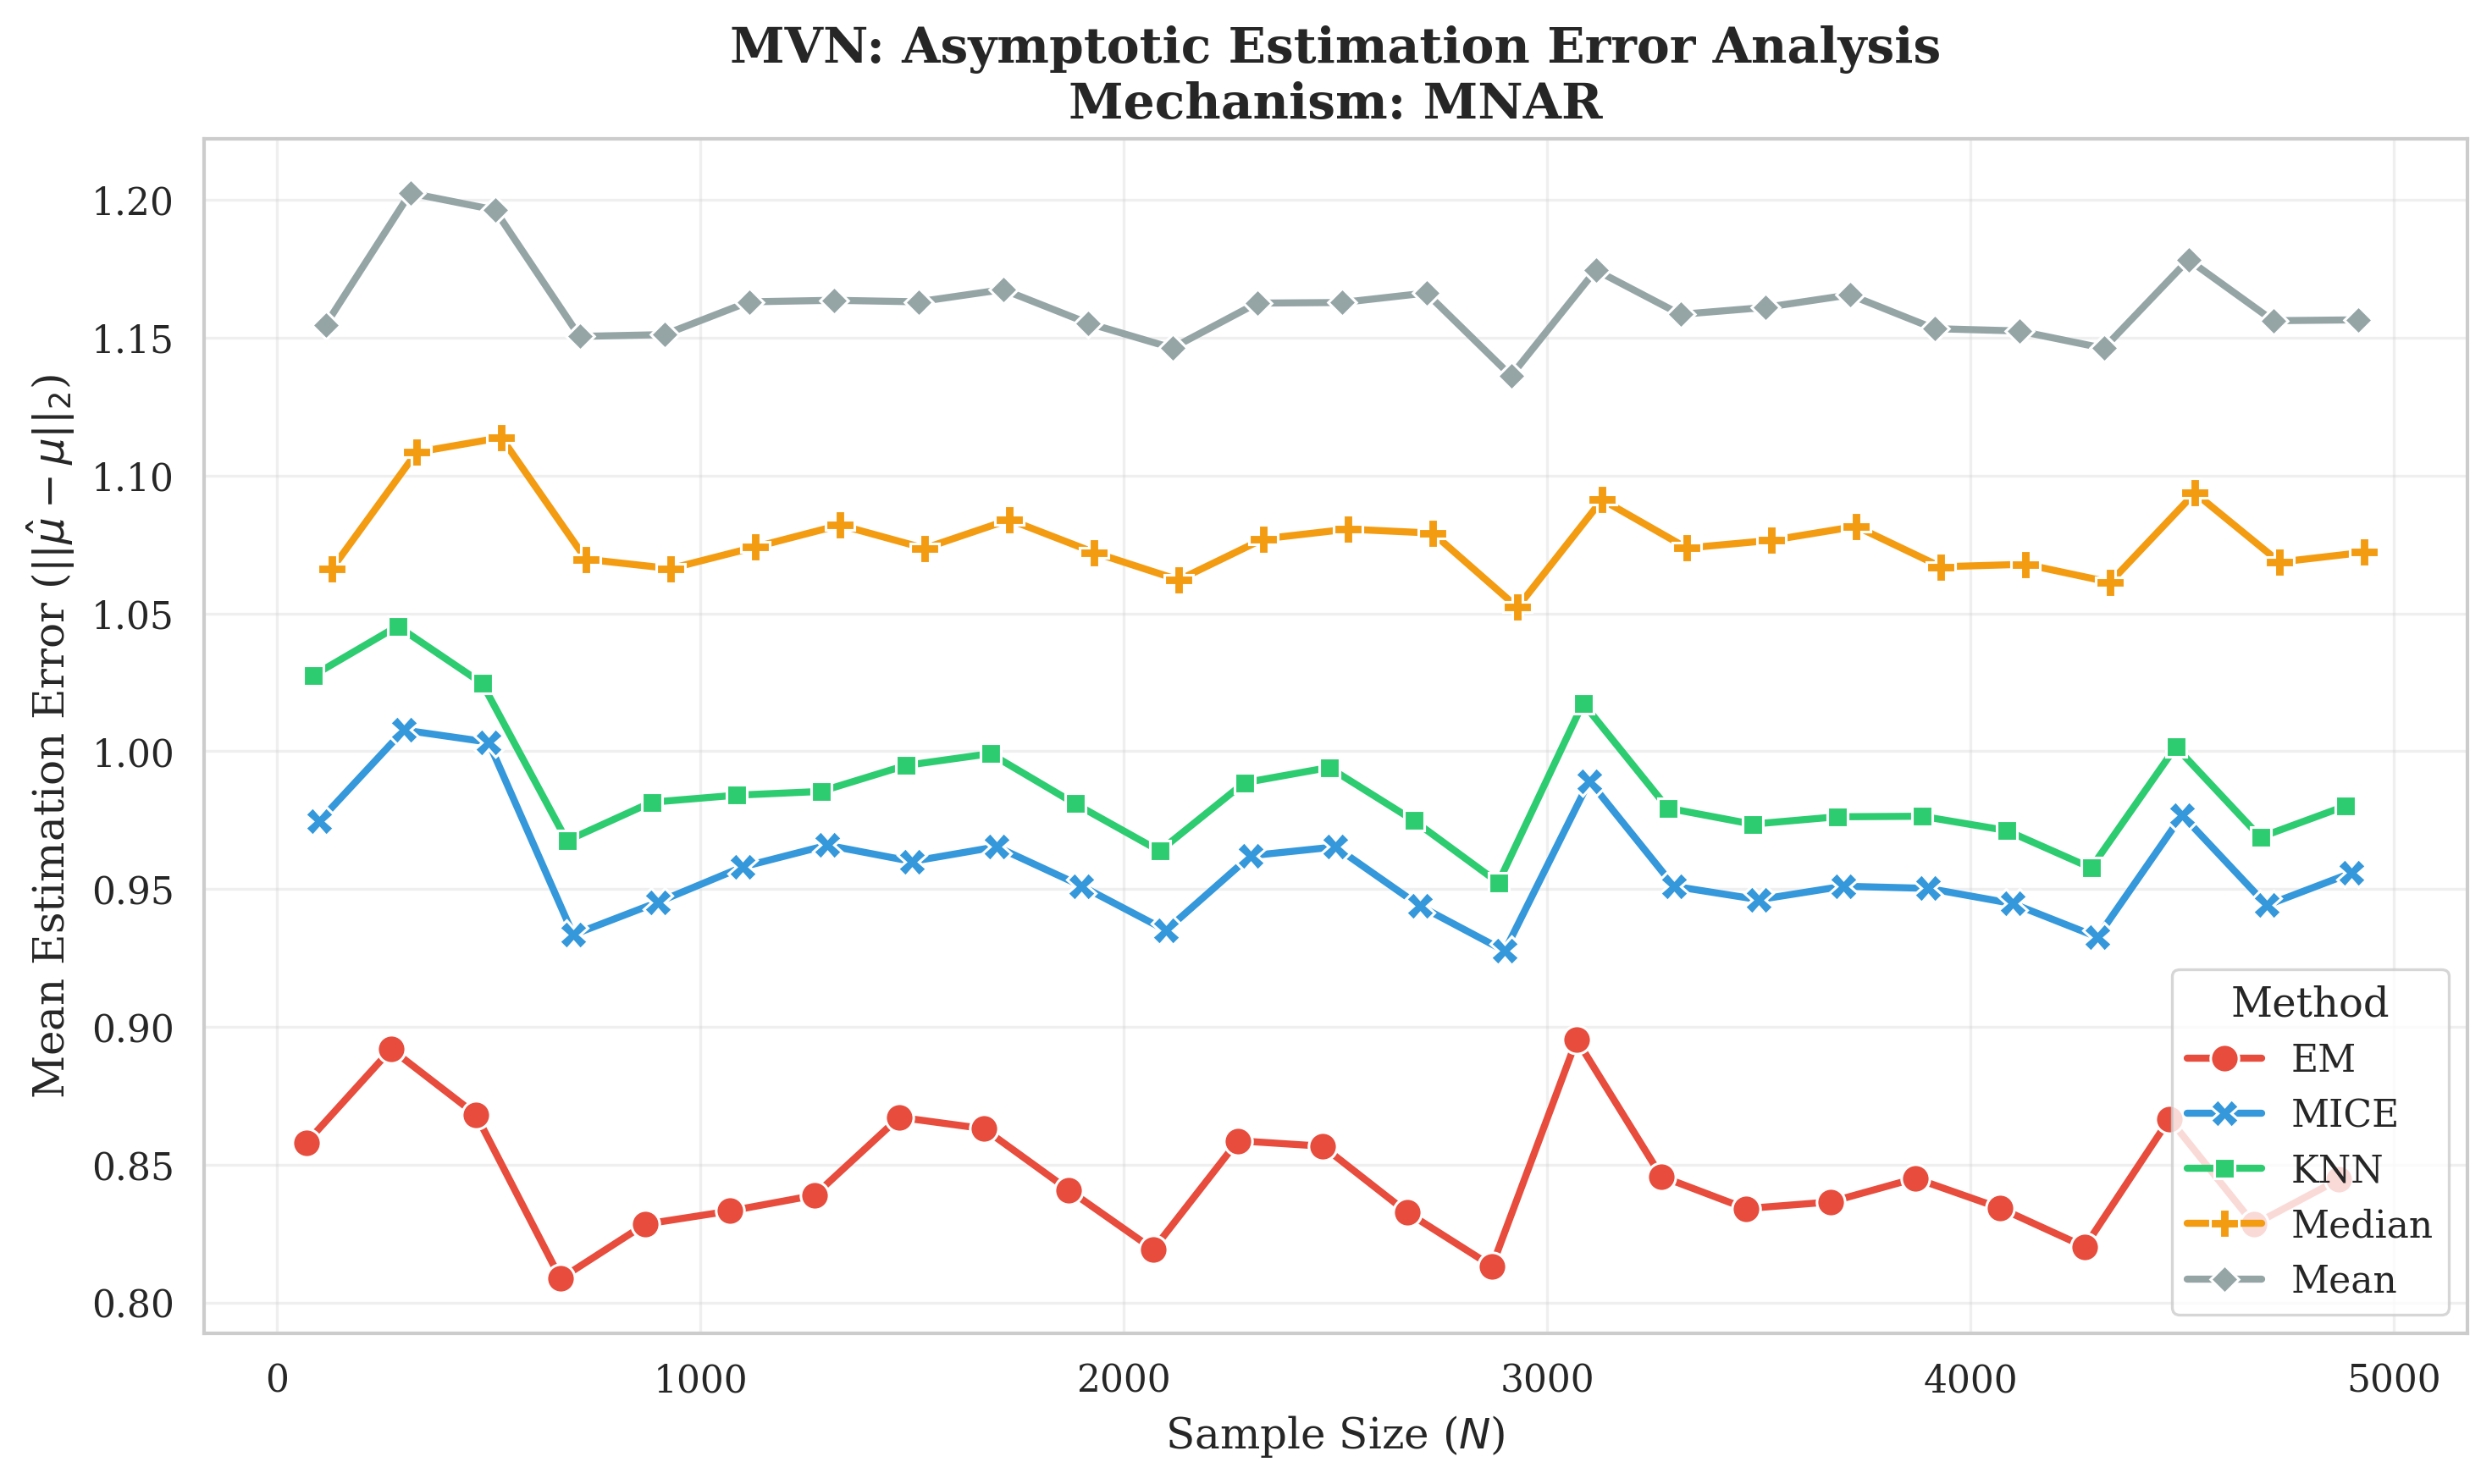
\includegraphics[width=0.8\textwidth]{plots/synthetic_multivariate/MNAR/sample_size_error_MNAR.png}
    \caption{Mean Estimation Error vs. Sample Size under MNAR. Note that standard deviation bars are omitted from the visualization to ensure clarity, as their magnitude ($\approx 0.1$) would obscure the trend lines.}
    \label{fig:mnar_asymptotic}
\end{figure}

As shown in Figure \ref{fig:mnar_asymptotic}, the error does not converge to zero as $n \to 5000$. Instead, all methods hit a ``bias floor.'' This empirically demonstrates that MNAR introduces a systematic bias that is asymptotically constant; simply collecting more data without correcting for the selection mechanism is futile.

\subsubsection{Computational Efficiency}
Finally, we evaluate the scalability of the algorithms. The reported execution times represent the average performance computed across all simulation parameters, aggregating results over the different covariance structures and missingness percentages. Figure \ref{fig:time_complexity} specifically illustrates the trends for the MAR mechanism; since the computational profiles for MCAR and MNAR are analogous, their respective plots are omitted here and can be found in the Appendix.
\begin{figure}[h!]
    \centering
    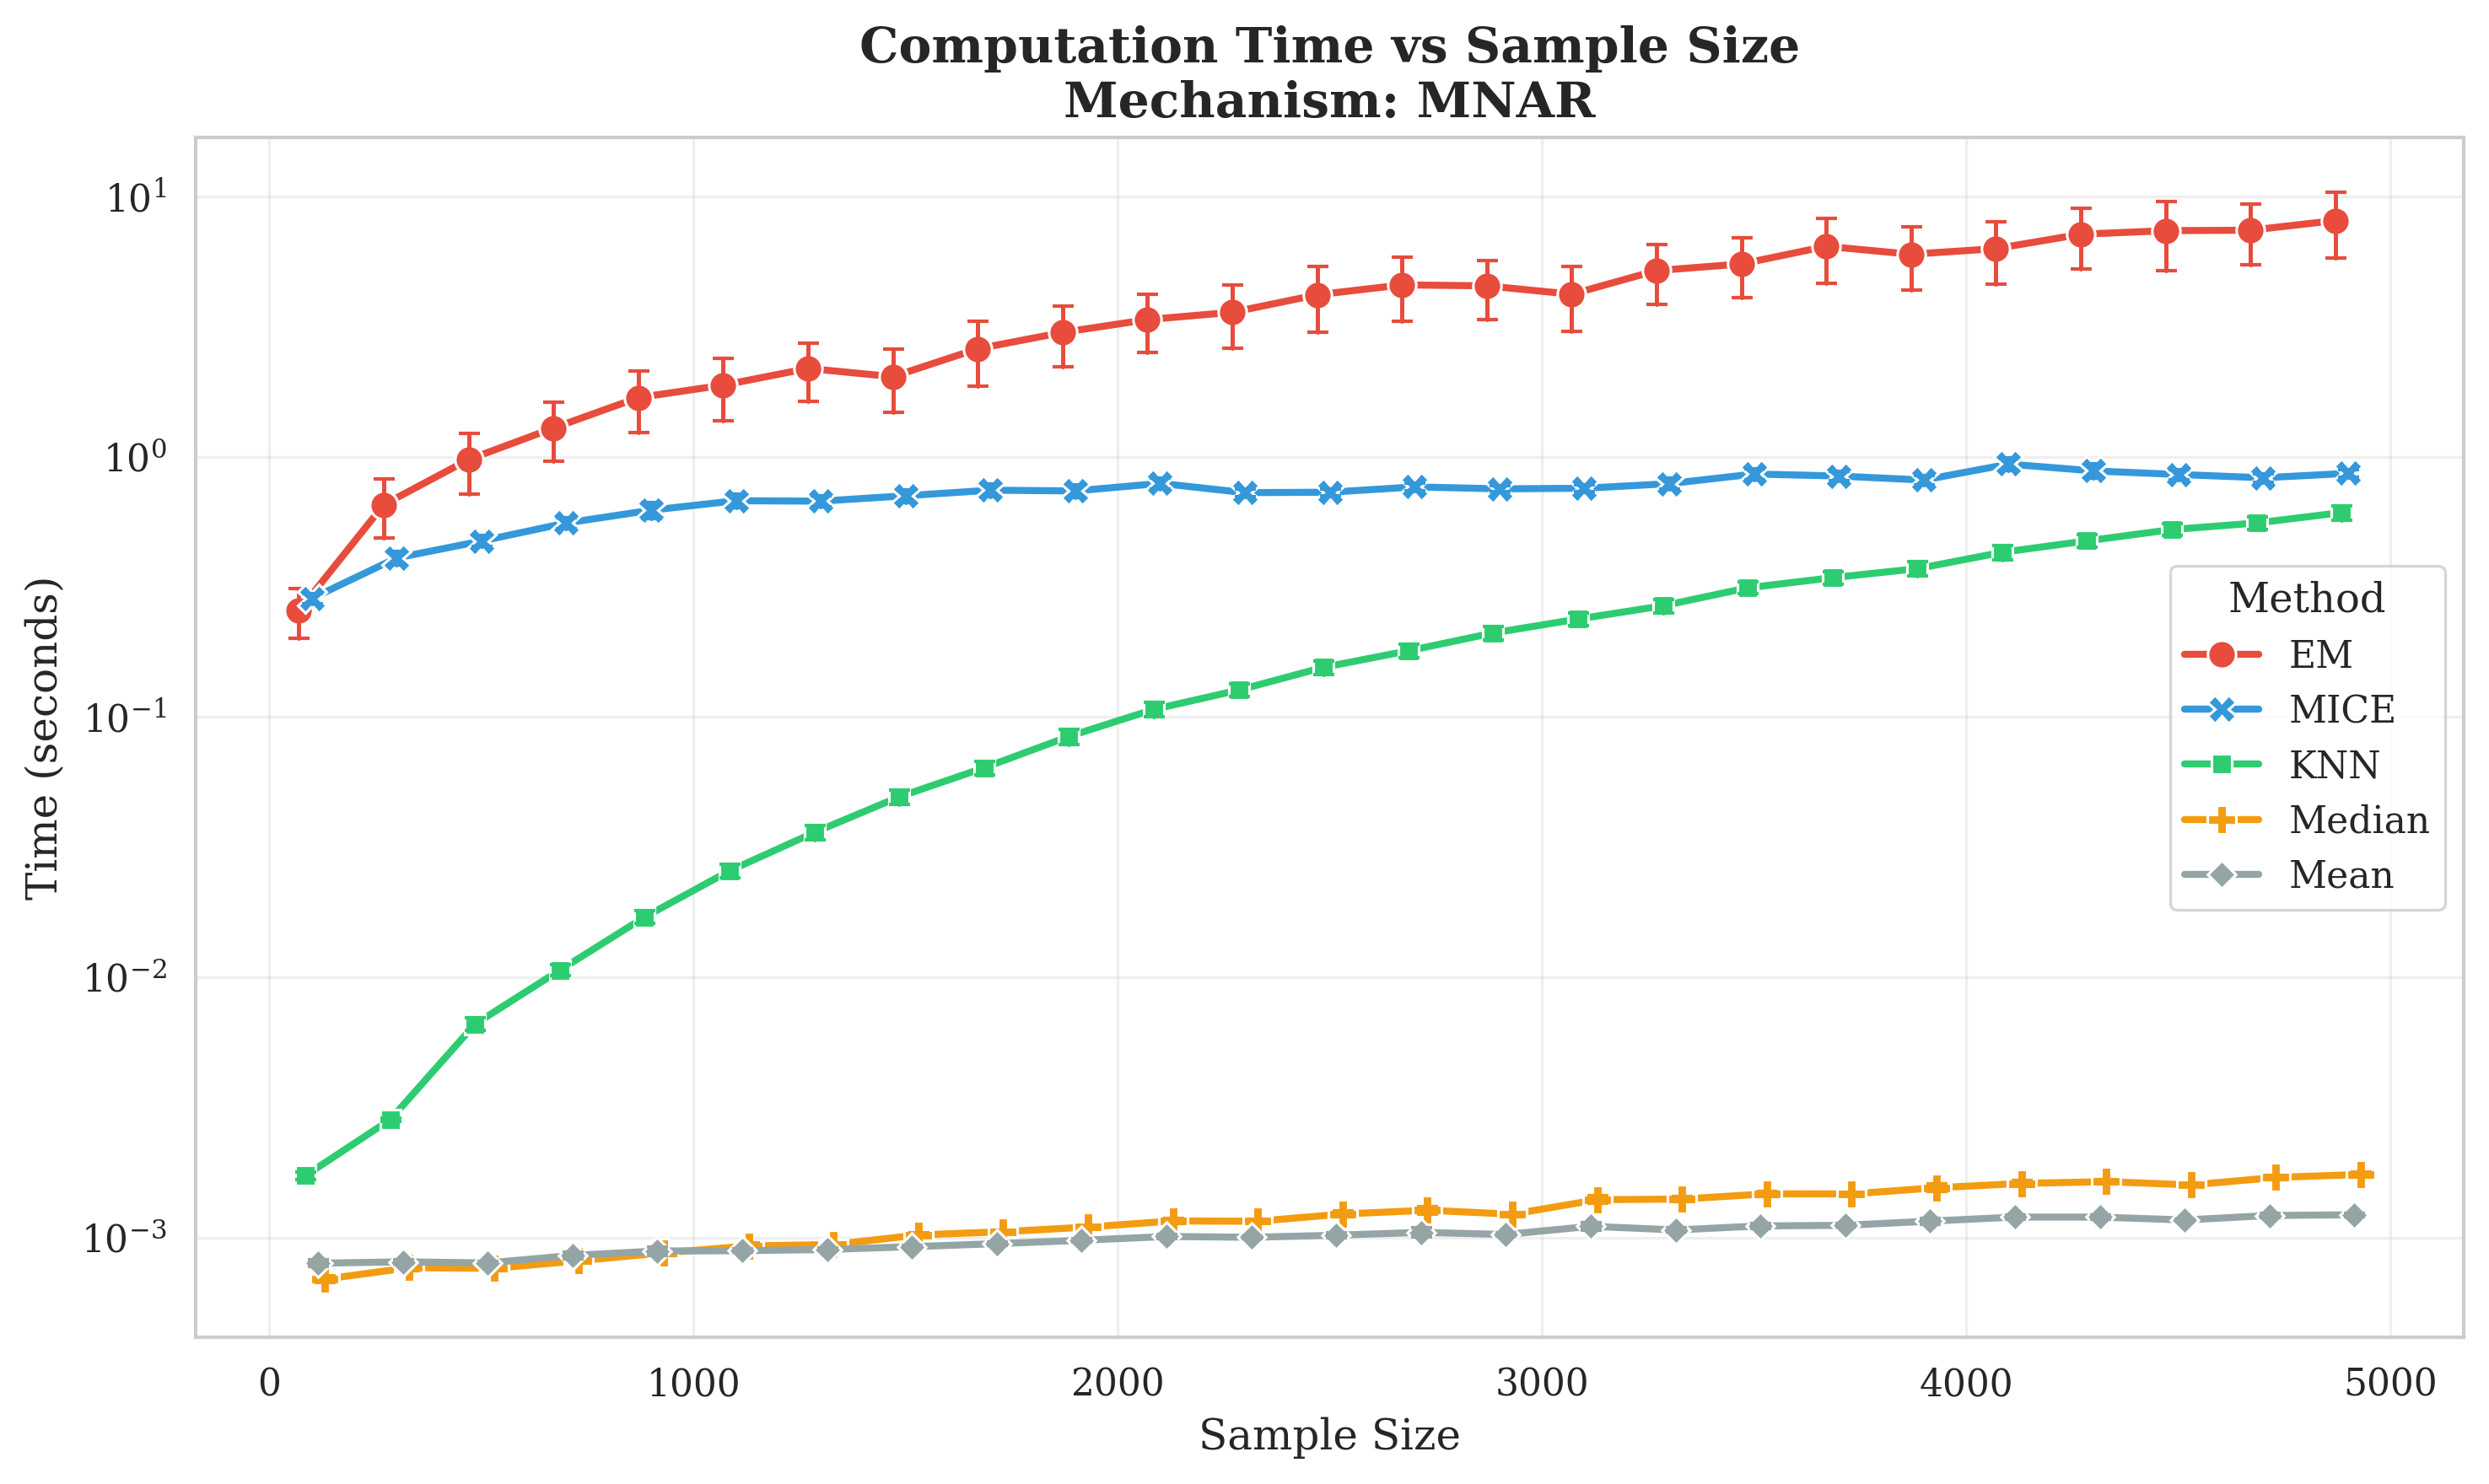
\includegraphics[width=0.8\textwidth]{plots/synthetic_multivariate/MNAR/sample_size_time_MNAR.png}
    \caption{\textbf{Computational Time vs. Sample Size (Log Scale).} The EM algorithm (red) incurs the highest absolute cost, though it remains manageable ($<15$s) for $N=5000$. kNN (green) is extremely fast but exhibits a steep relative growth rate due to distance matrix calculations. MICE (blue) remains stable around 1 second.}
    \label{fig:time_complexity}
\end{figure}

While heuristic methods (Mean, Median) are computationally negligible, the \textbf{EM algorithm} (red) incurs the highest absolute cost. Despite this, the execution time remains viable for mid-sized datasets, reaching approximately 15 seconds for $N=5000$. 

Notably, kNN (green) demonstrates the most rapid rate of growth—spanning three orders of magnitude from $N=100$ to $N=5000$—which reflects the theoretical quadratic complexity of neighbor search. However, due to the low constant factors, it remains sub-second in absolute terms for this range. MICE (blue) occupies a middle ground, showing a stable and moderate cost ($\approx 1$ second), likely due to the fixed number of iterations and the efficiency of Random Forests on low-dimensional data ($p=5$).


% --- SECTION 4.2: GMM RESULTS ---
\subsection{GMM Performance with Missing Labels}

In the Gaussian Mixture Model (GMM) setting, we evaluated the algorithms' ability to recover the true class mixing weights ($\boldsymbol{\pi}$) when a significant portion of the class labels is missing. We analyzed the performance across the four structural configurations defined in Section 3.1, varying the percentage of missing labels from 10\% to 70\% in a $p=5$ dimensional space.

\subsubsection{Global Sensitivity to Missing Labels}
First, we analyze the overall robustness of the methods. 

\textit{Note on Aggregation: The data presented in Figure \ref{fig:gmm_heatmap} are obtained by averaging the Proportion Estimation Error ($E_{\pi}$) across all simulation parameters (sample sizes $N \in [100, 5000]$ and all structural configurations).}

\begin{figure}[h!]
    \centering
    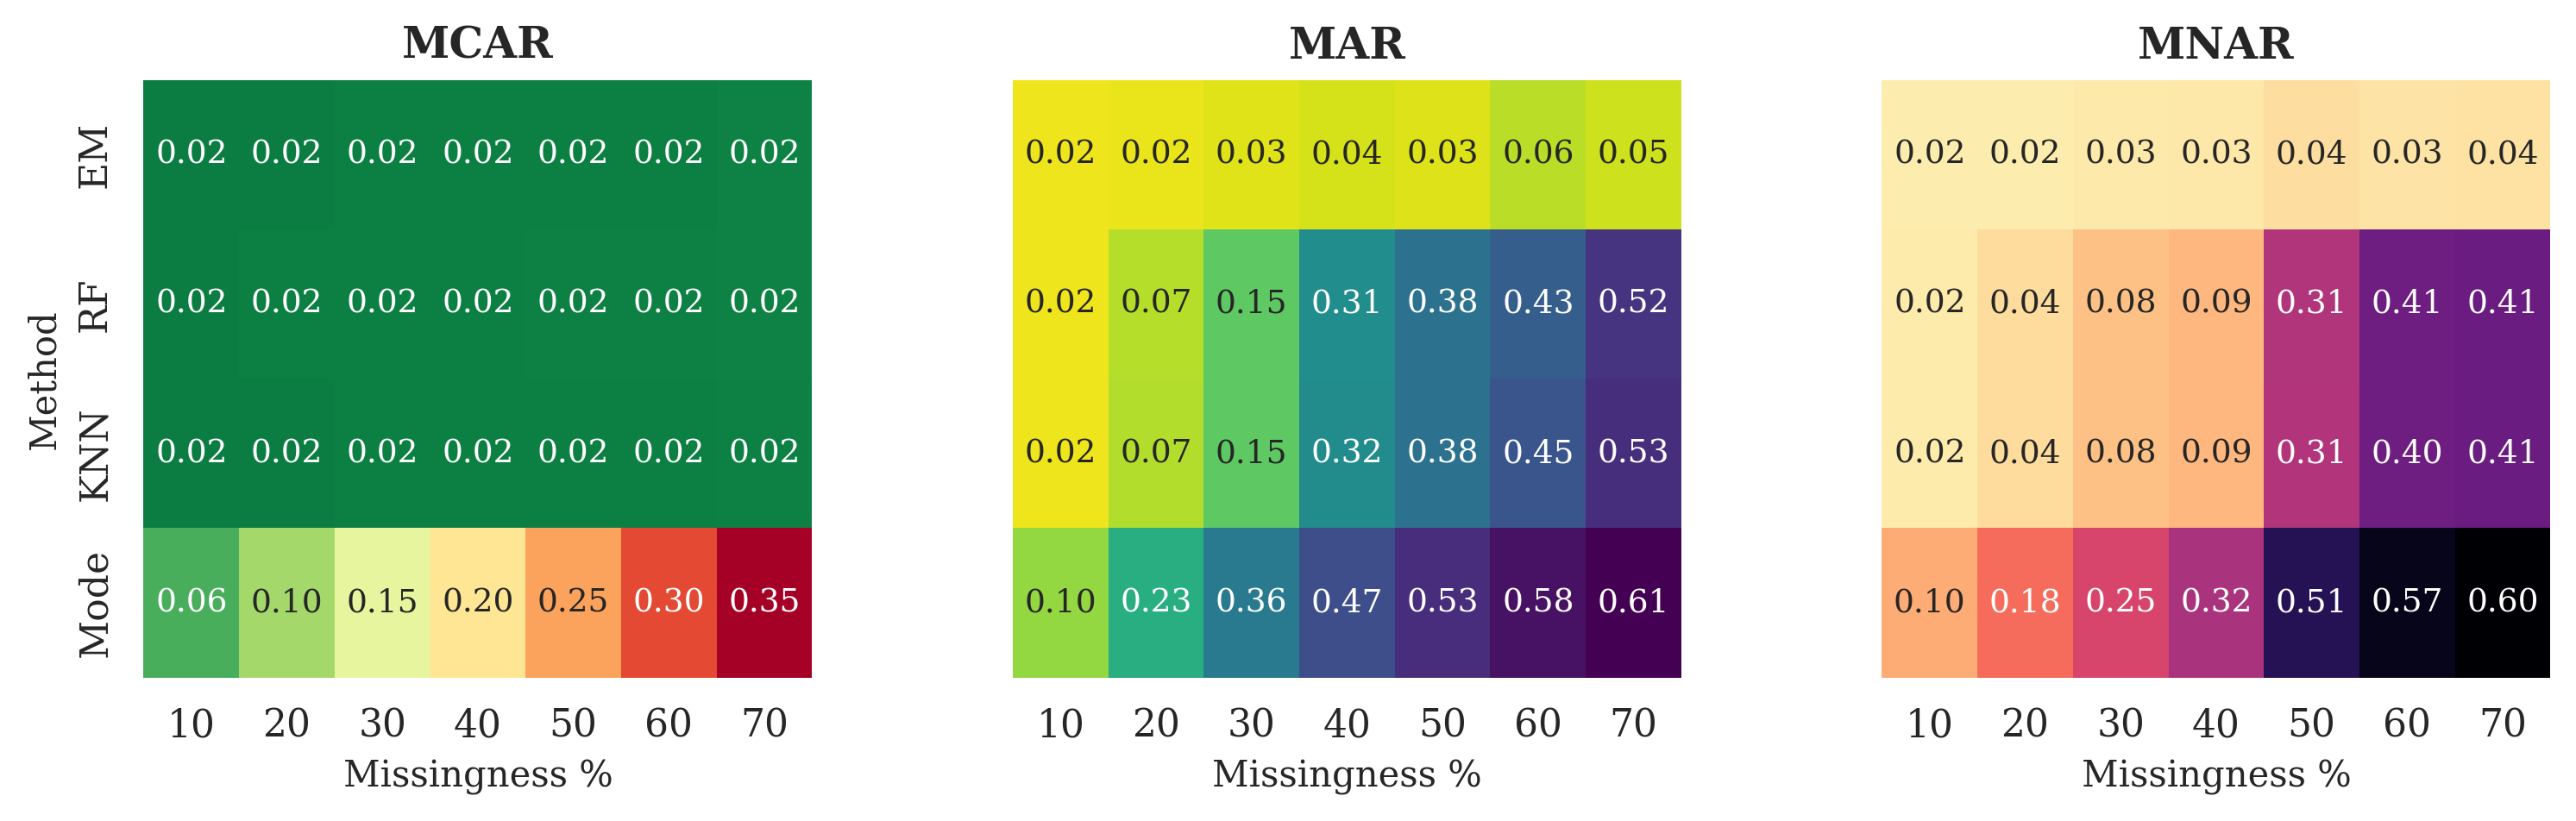
\includegraphics[width=1.0\textwidth]{plots/synthetic_gmm/error_heatmap_all_gmm.png}
    \caption{\textbf{Global Proportion Estimation Error.} The heatmap compares the stability of EM against imputation methods (RF, kNN). EM remains robust (green) even at 70\% missingness, whereas RF and kNN degrade linearly.}
    \label{fig:gmm_heatmap}
\end{figure}

The EM algorithm (top row) exhibits remarkable stability, maintaining an average error $E_{\pi} < 0.05$ even when 70\% of the data is unlabeled. Conversely, imputation methods like Random Forest and kNN (middle/bottom rows) degrade linearly, with errors exceeding $0.40$ in high-missingness regimes.

\subsubsection{Structural Analysis: Geometry and Overlap}
To understand the specific conditions driving these results, we decomposed the performance based on the data's topological structure.

\textit{Note on Aggregation: The panels in Figure \ref{fig:gmm_combined} display the error trends for specific structural subsets, averaging results over all sample sizes.}

\begin{figure}[H]
    \centering
    % Row 1: Separation and Overlap
    \begin{subfigure}[b]{0.48\textwidth}
        \centering
        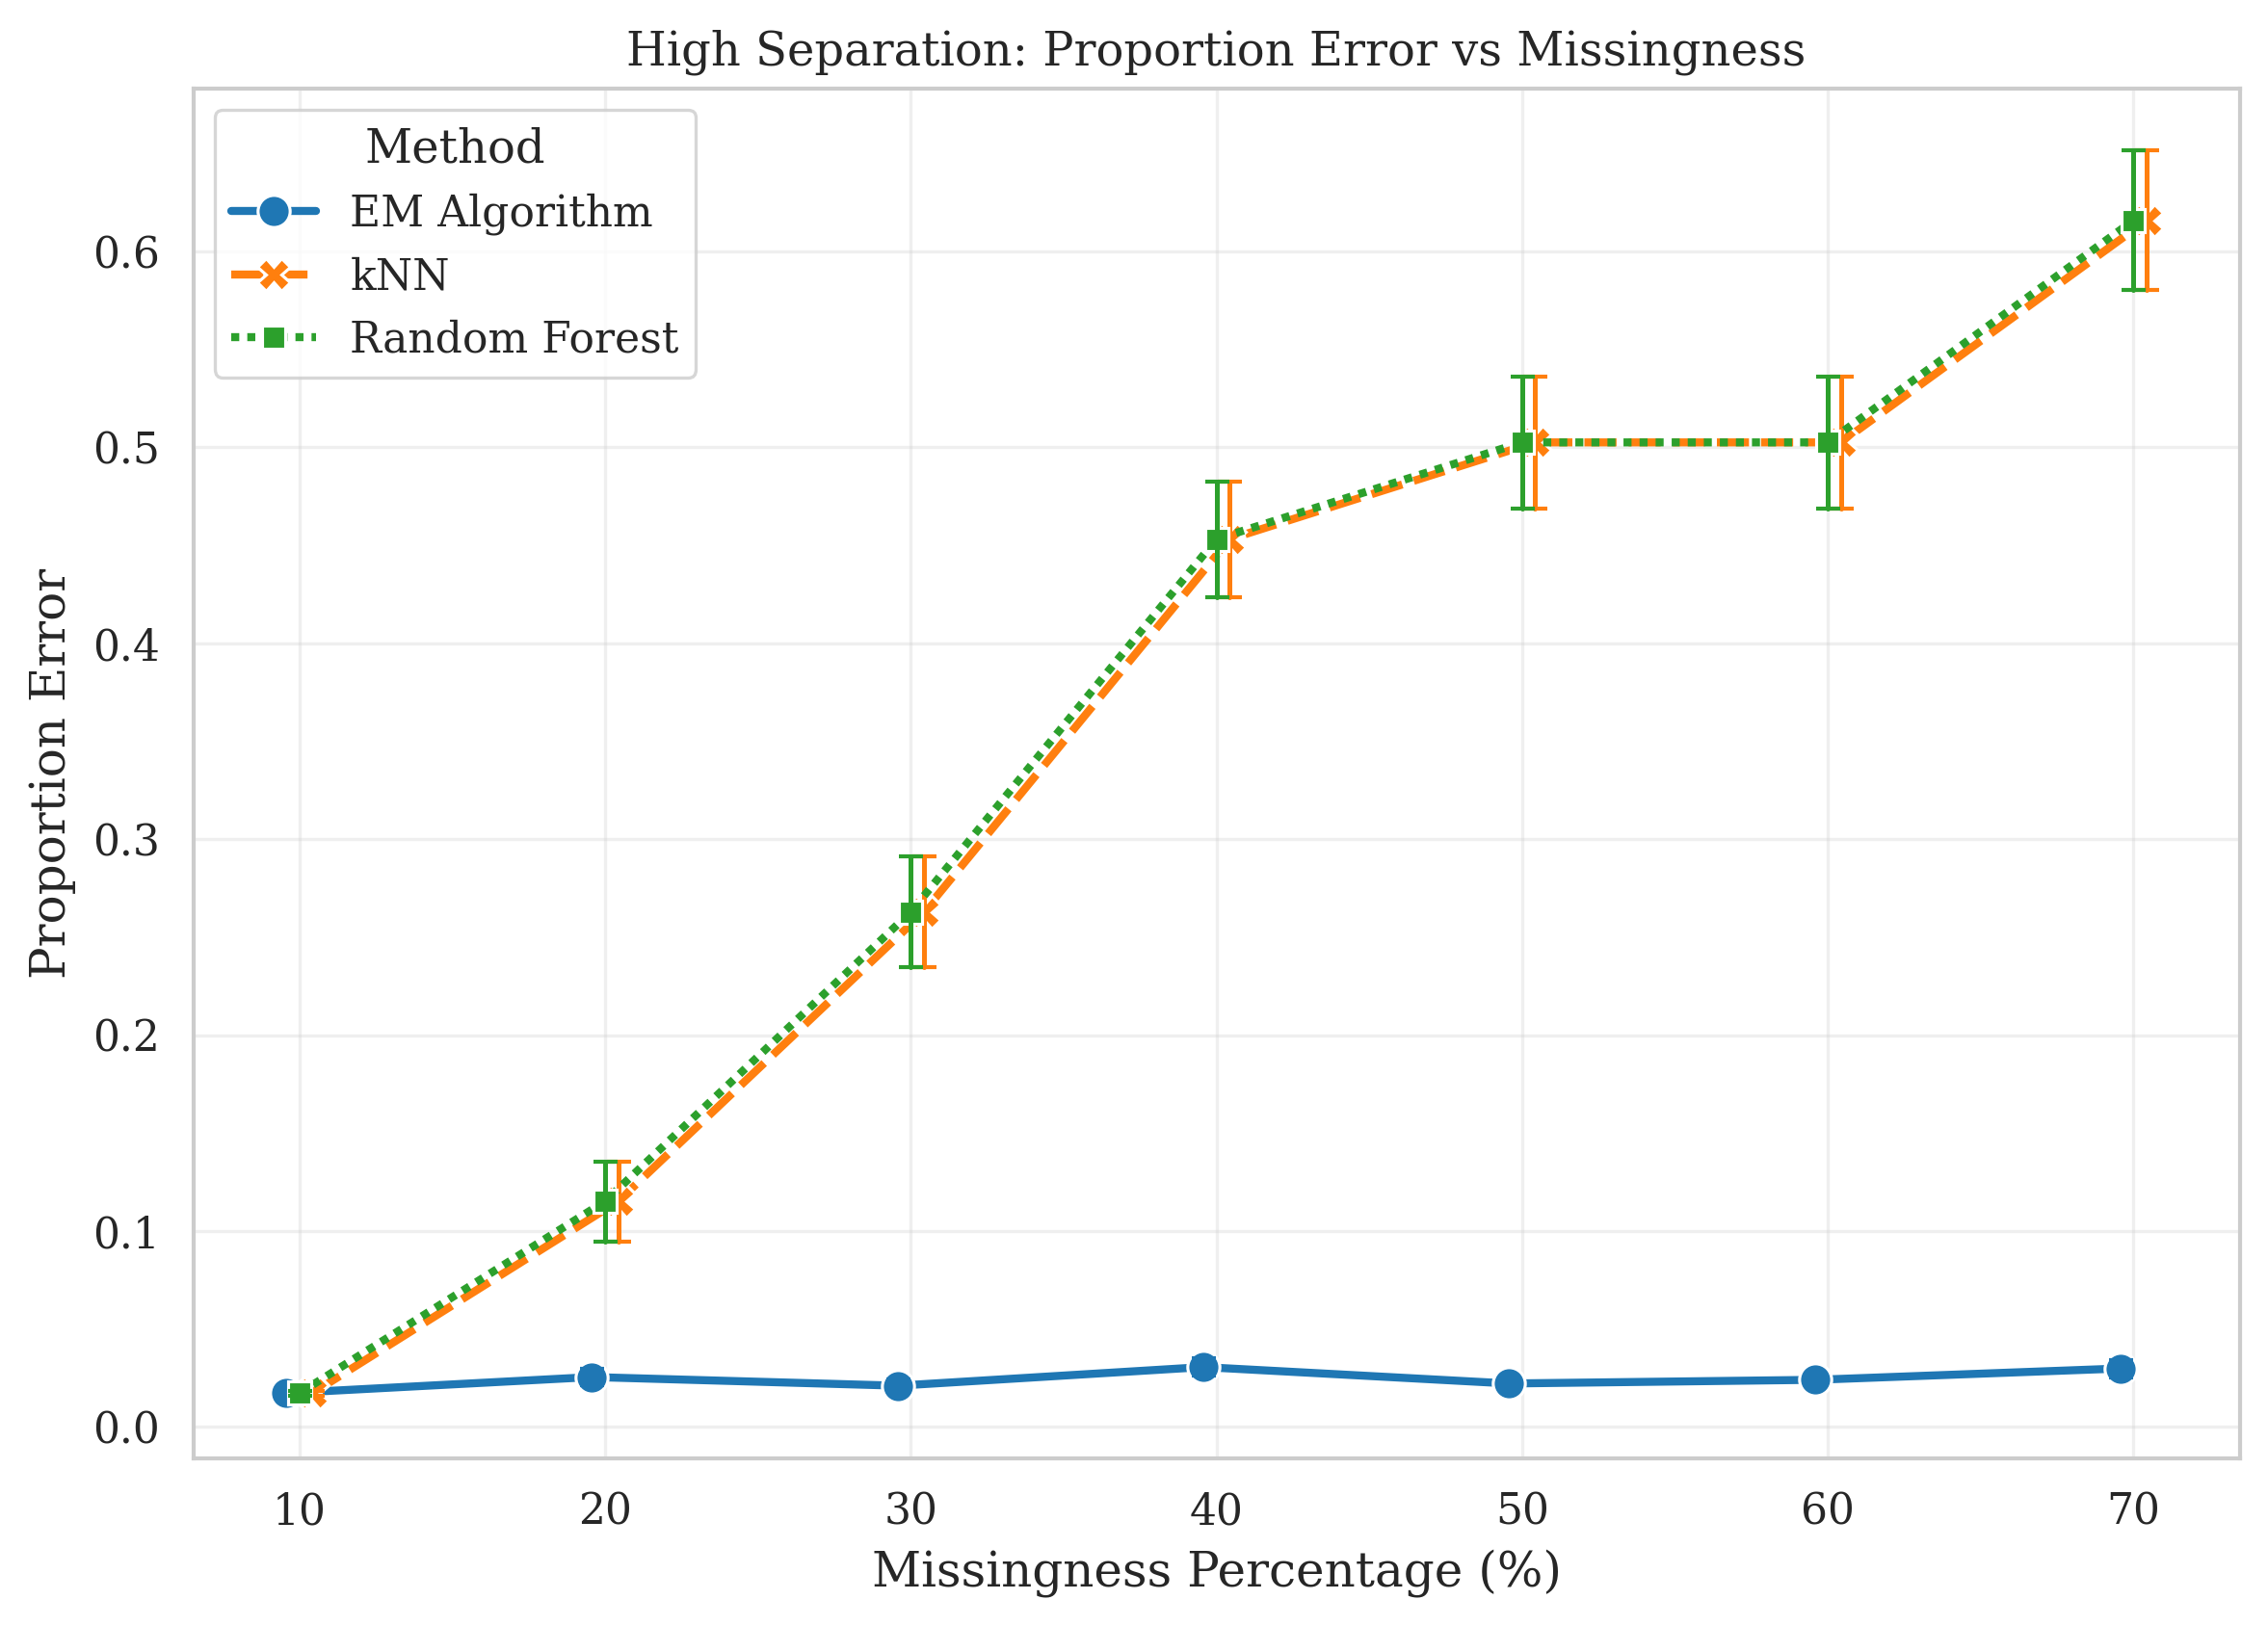
\includegraphics[width=\textwidth]{plots/additional_visualizations/gmm_clustering_scenarios/GMM_Separation.png}
        \caption{\textbf{High Separation}}
    \end{subfigure}
    \hfill
    \begin{subfigure}[b]{0.48\textwidth}
        \centering
        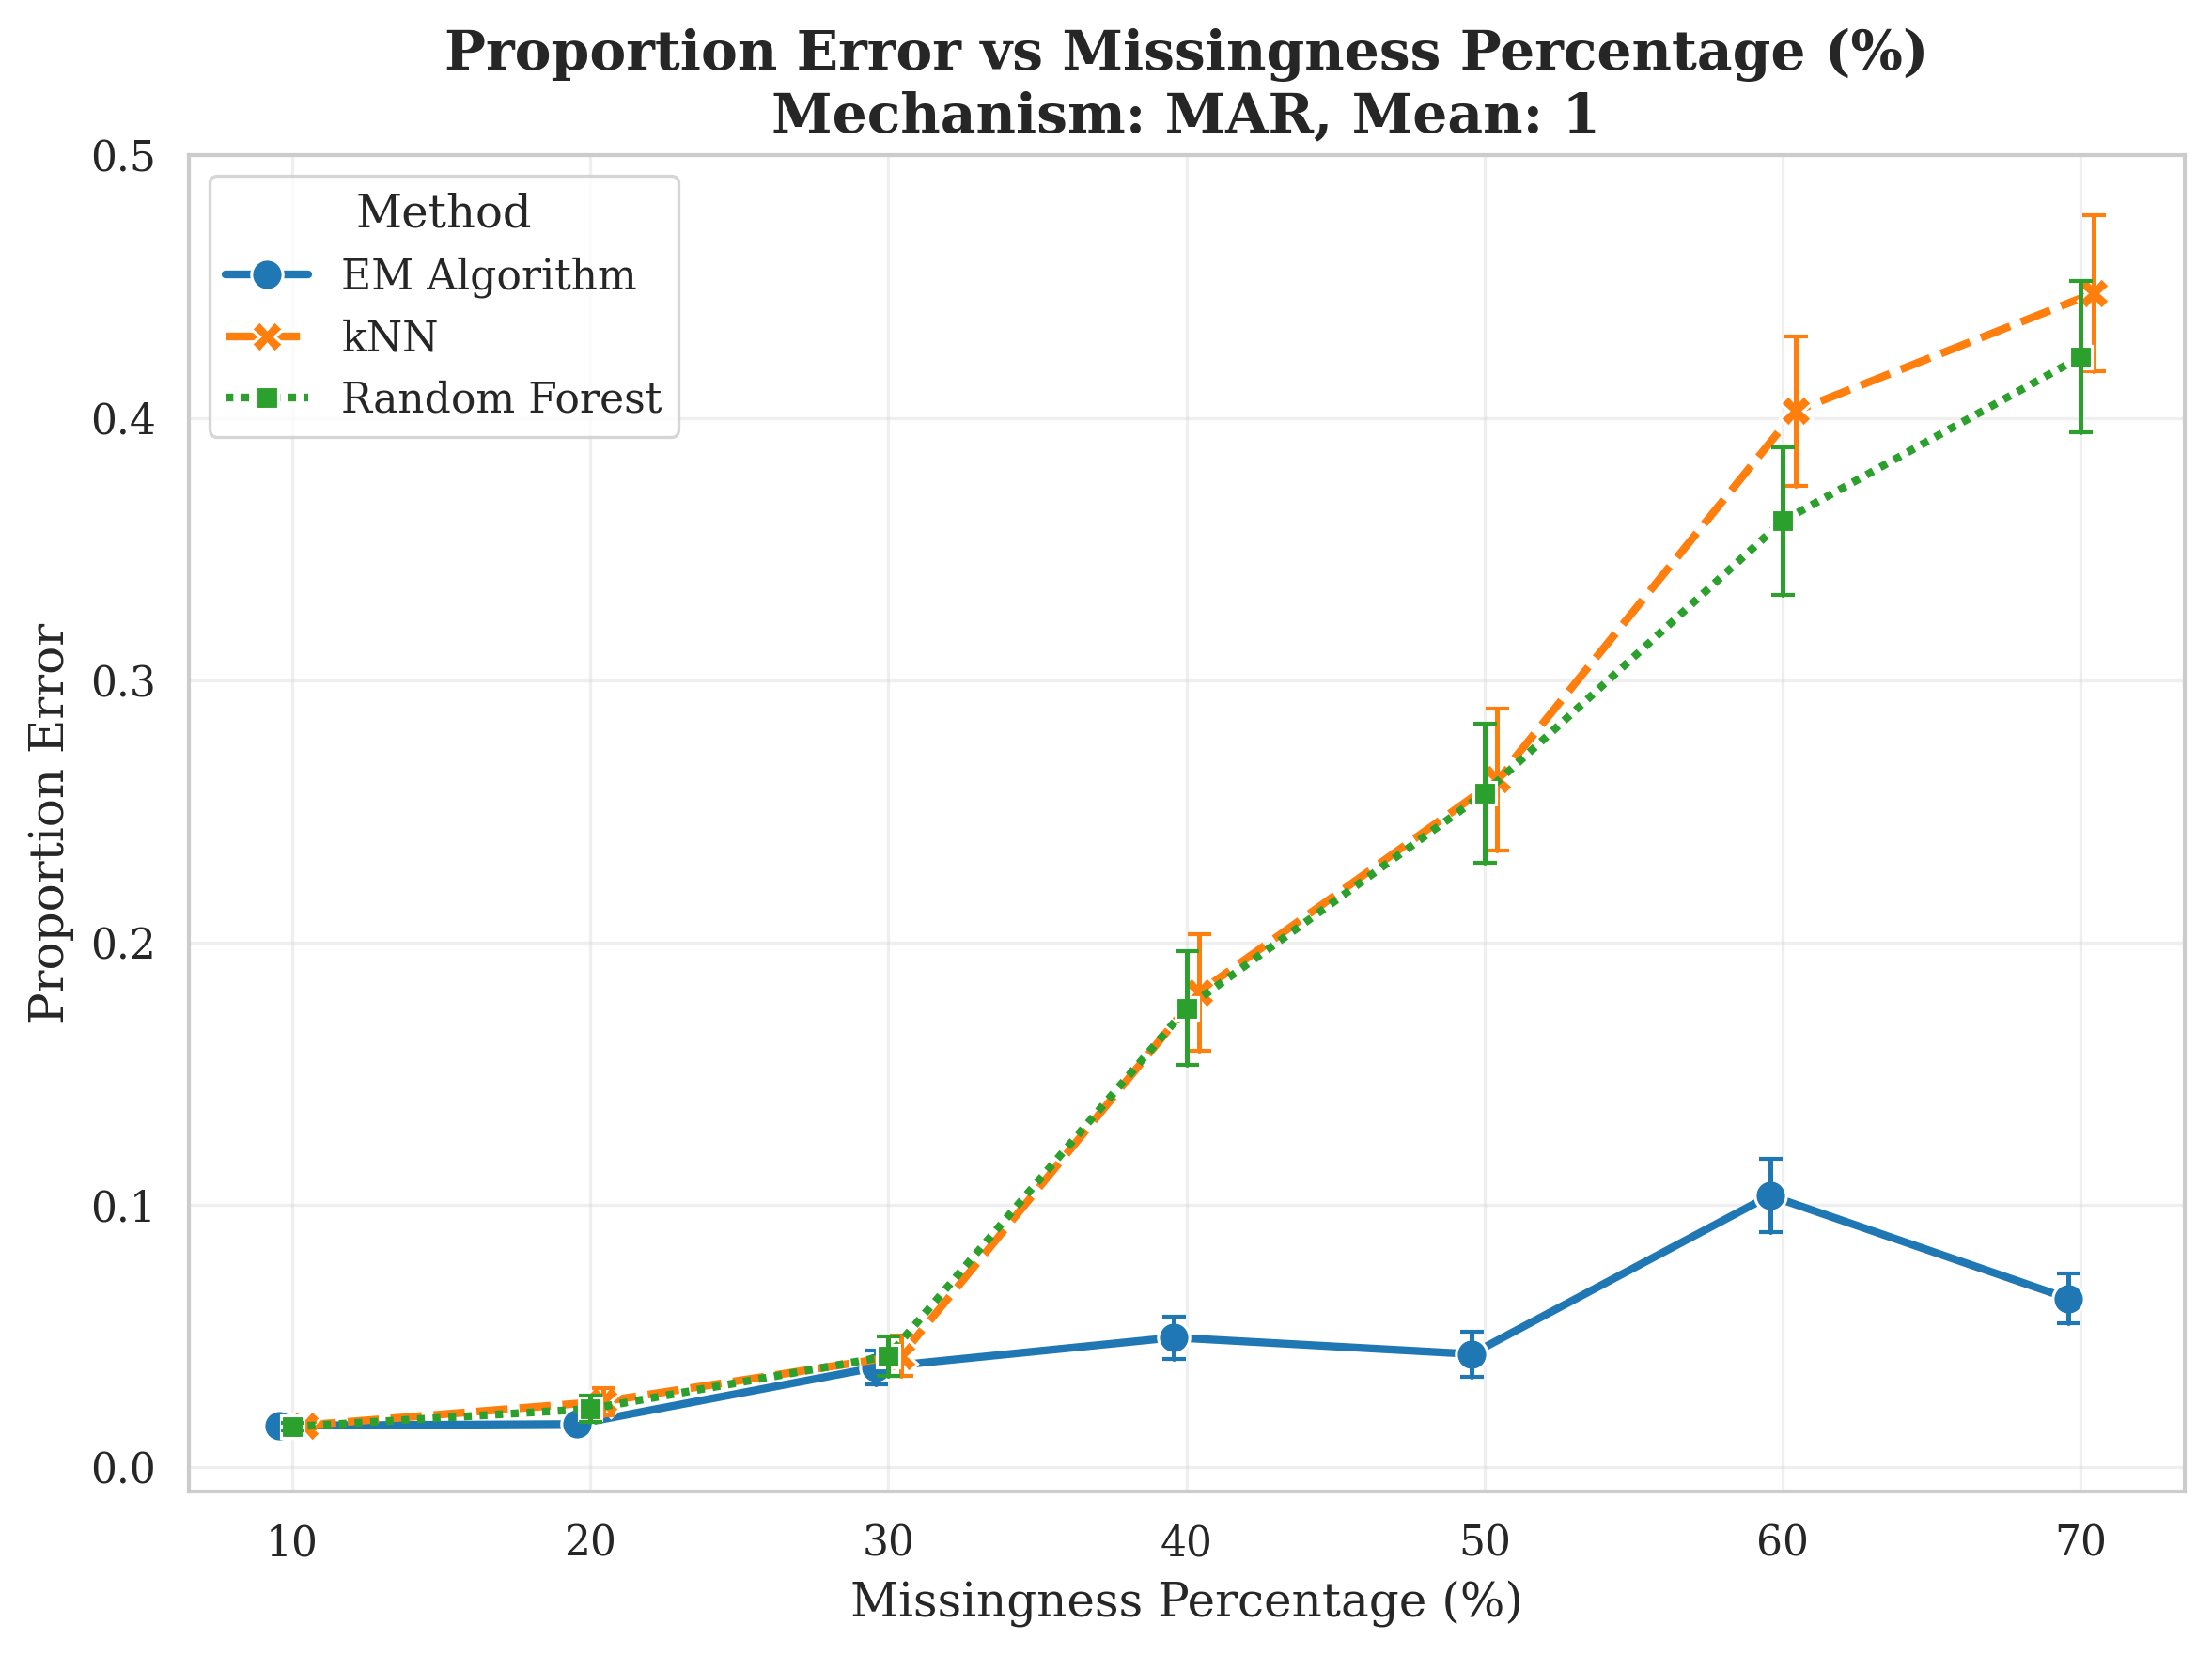
\includegraphics[width=\textwidth]{plots/additional_visualizations/gmm_clustering_scenarios/GMM_Overlap.png}
        \caption{\textbf{High Overlap}}
    \end{subfigure}
    
    \vspace{1em}
    
    % Row 2: Imbalanced and Heterogeneous
    \begin{subfigure}[b]{0.48\textwidth}
        \centering
        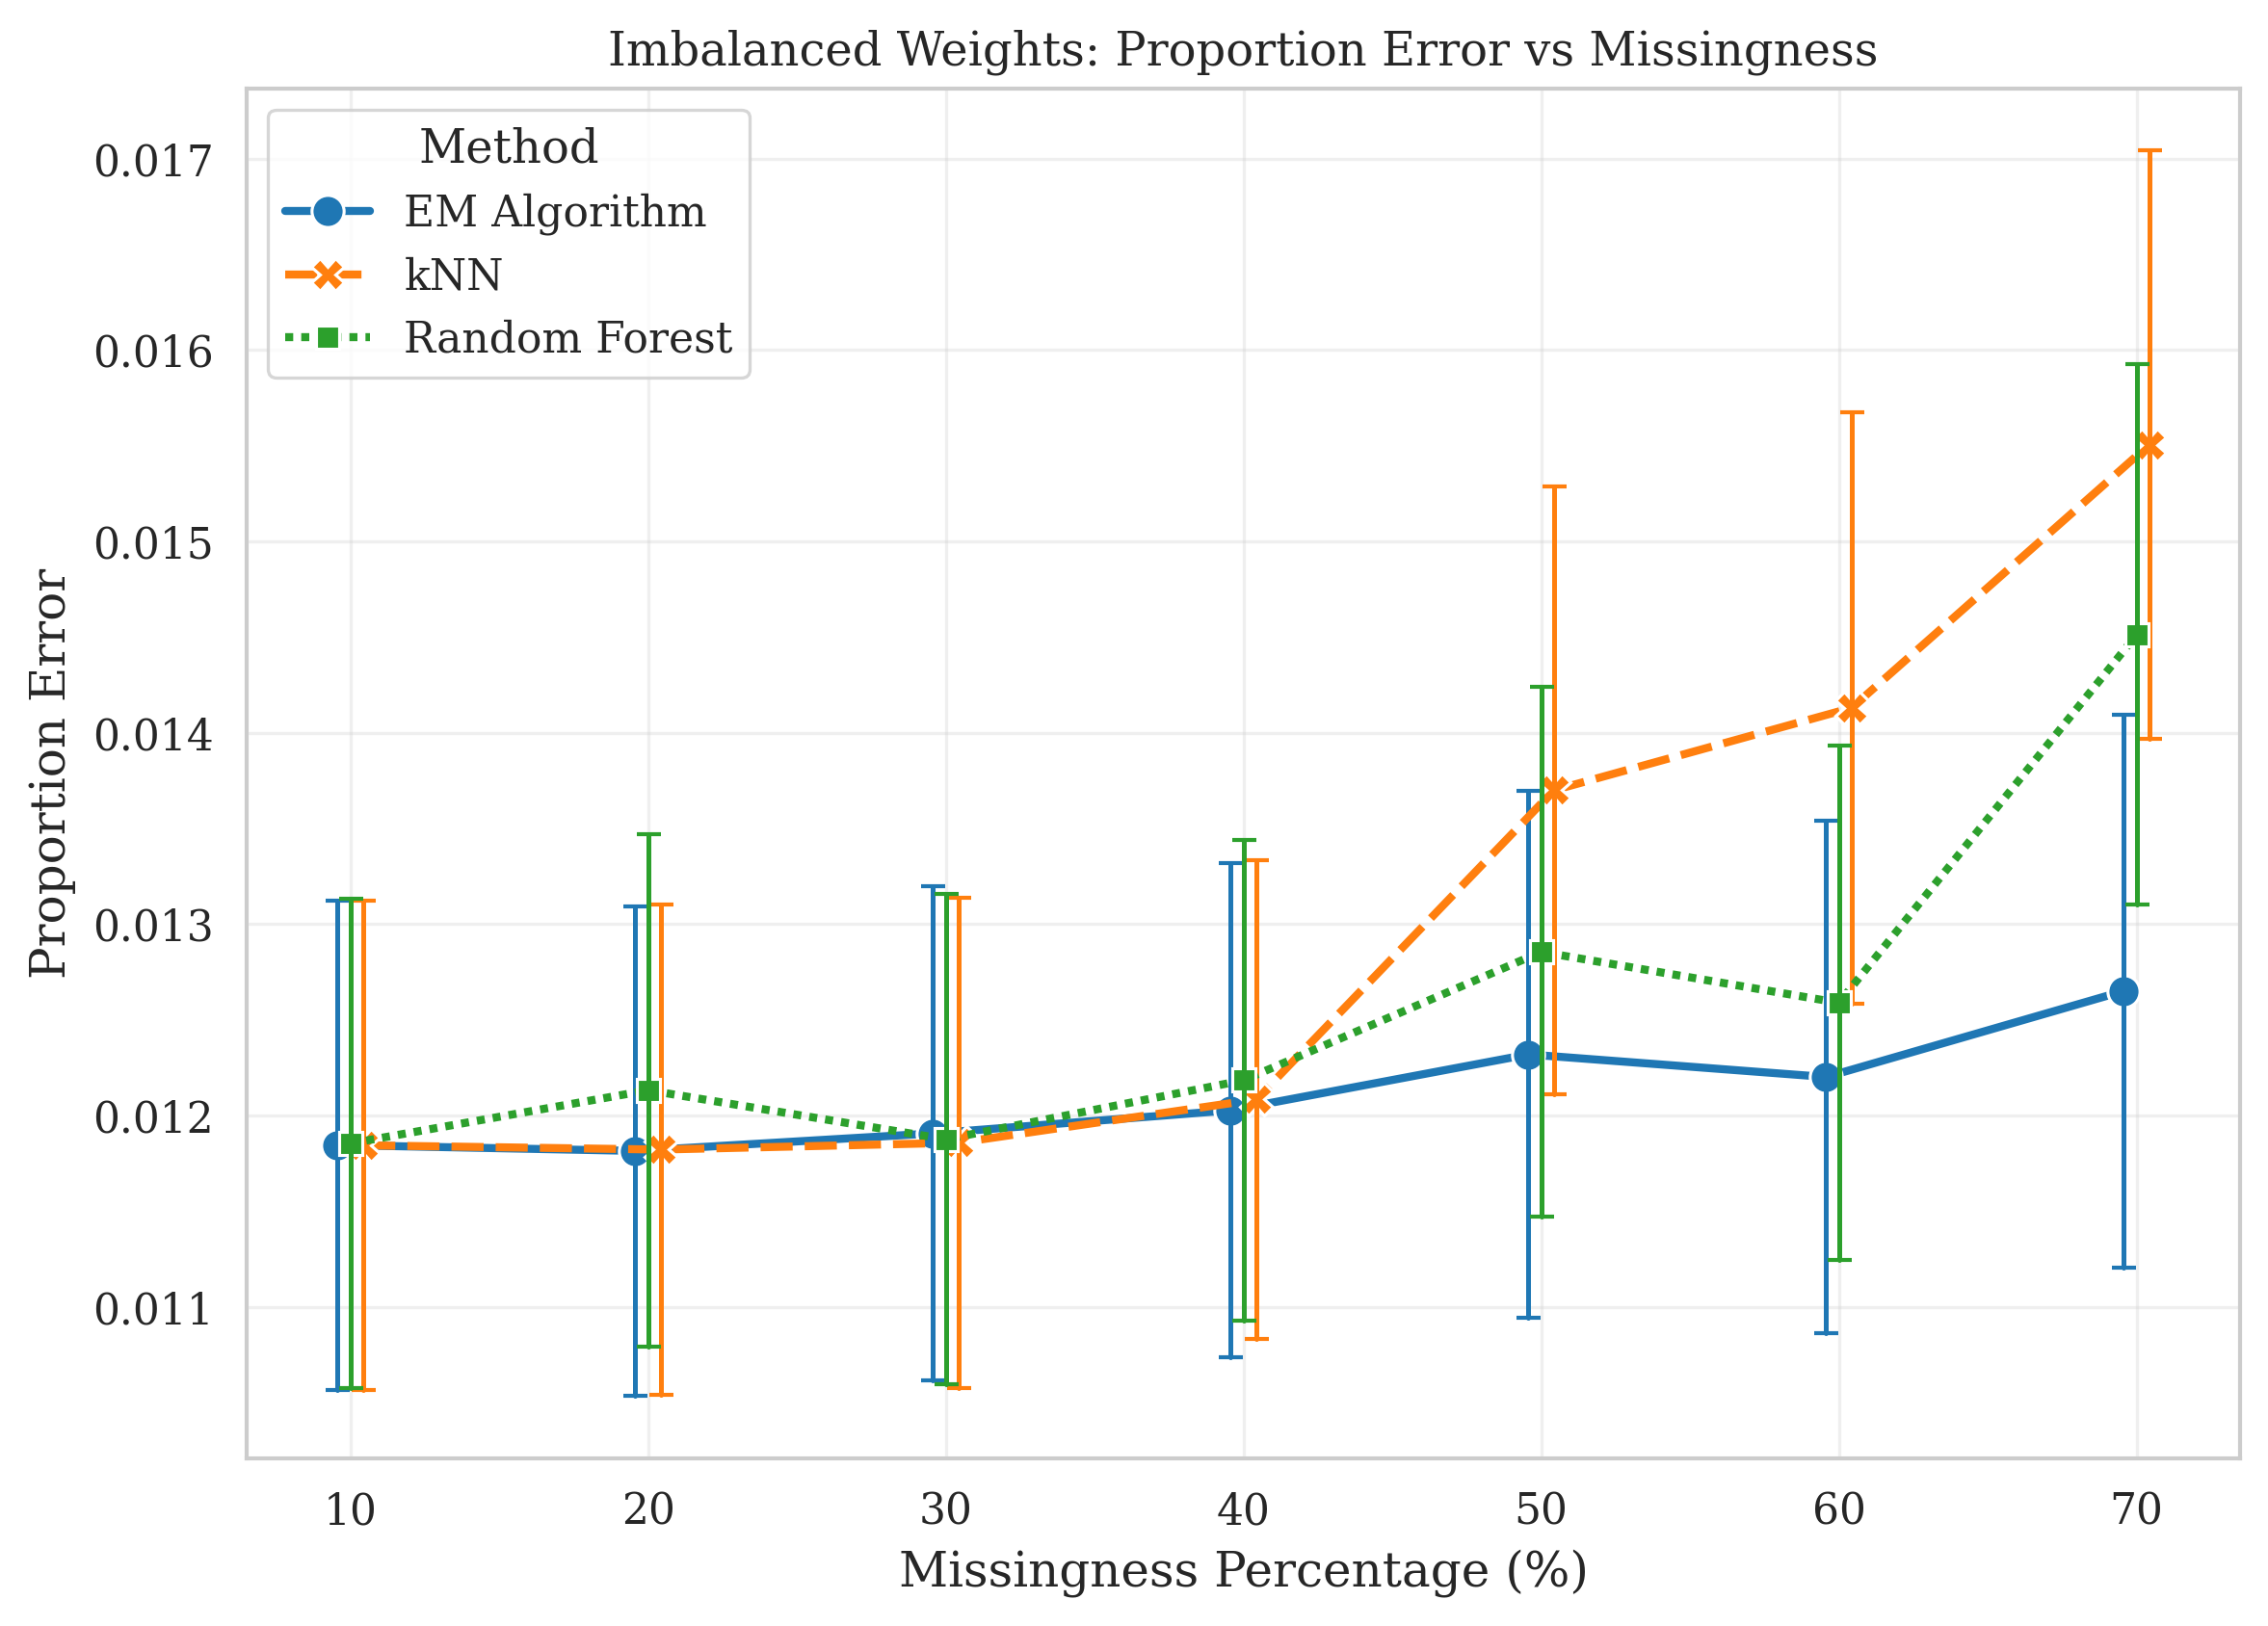
\includegraphics[width=\textwidth]{plots/additional_visualizations/gmm_clustering_scenarios/gmm_imbalanced_weights.png}
        \caption{\textbf{Imbalanced Weights}}
    \end{subfigure}
    \hfill
    \begin{subfigure}[b]{0.48\textwidth}
        \centering
        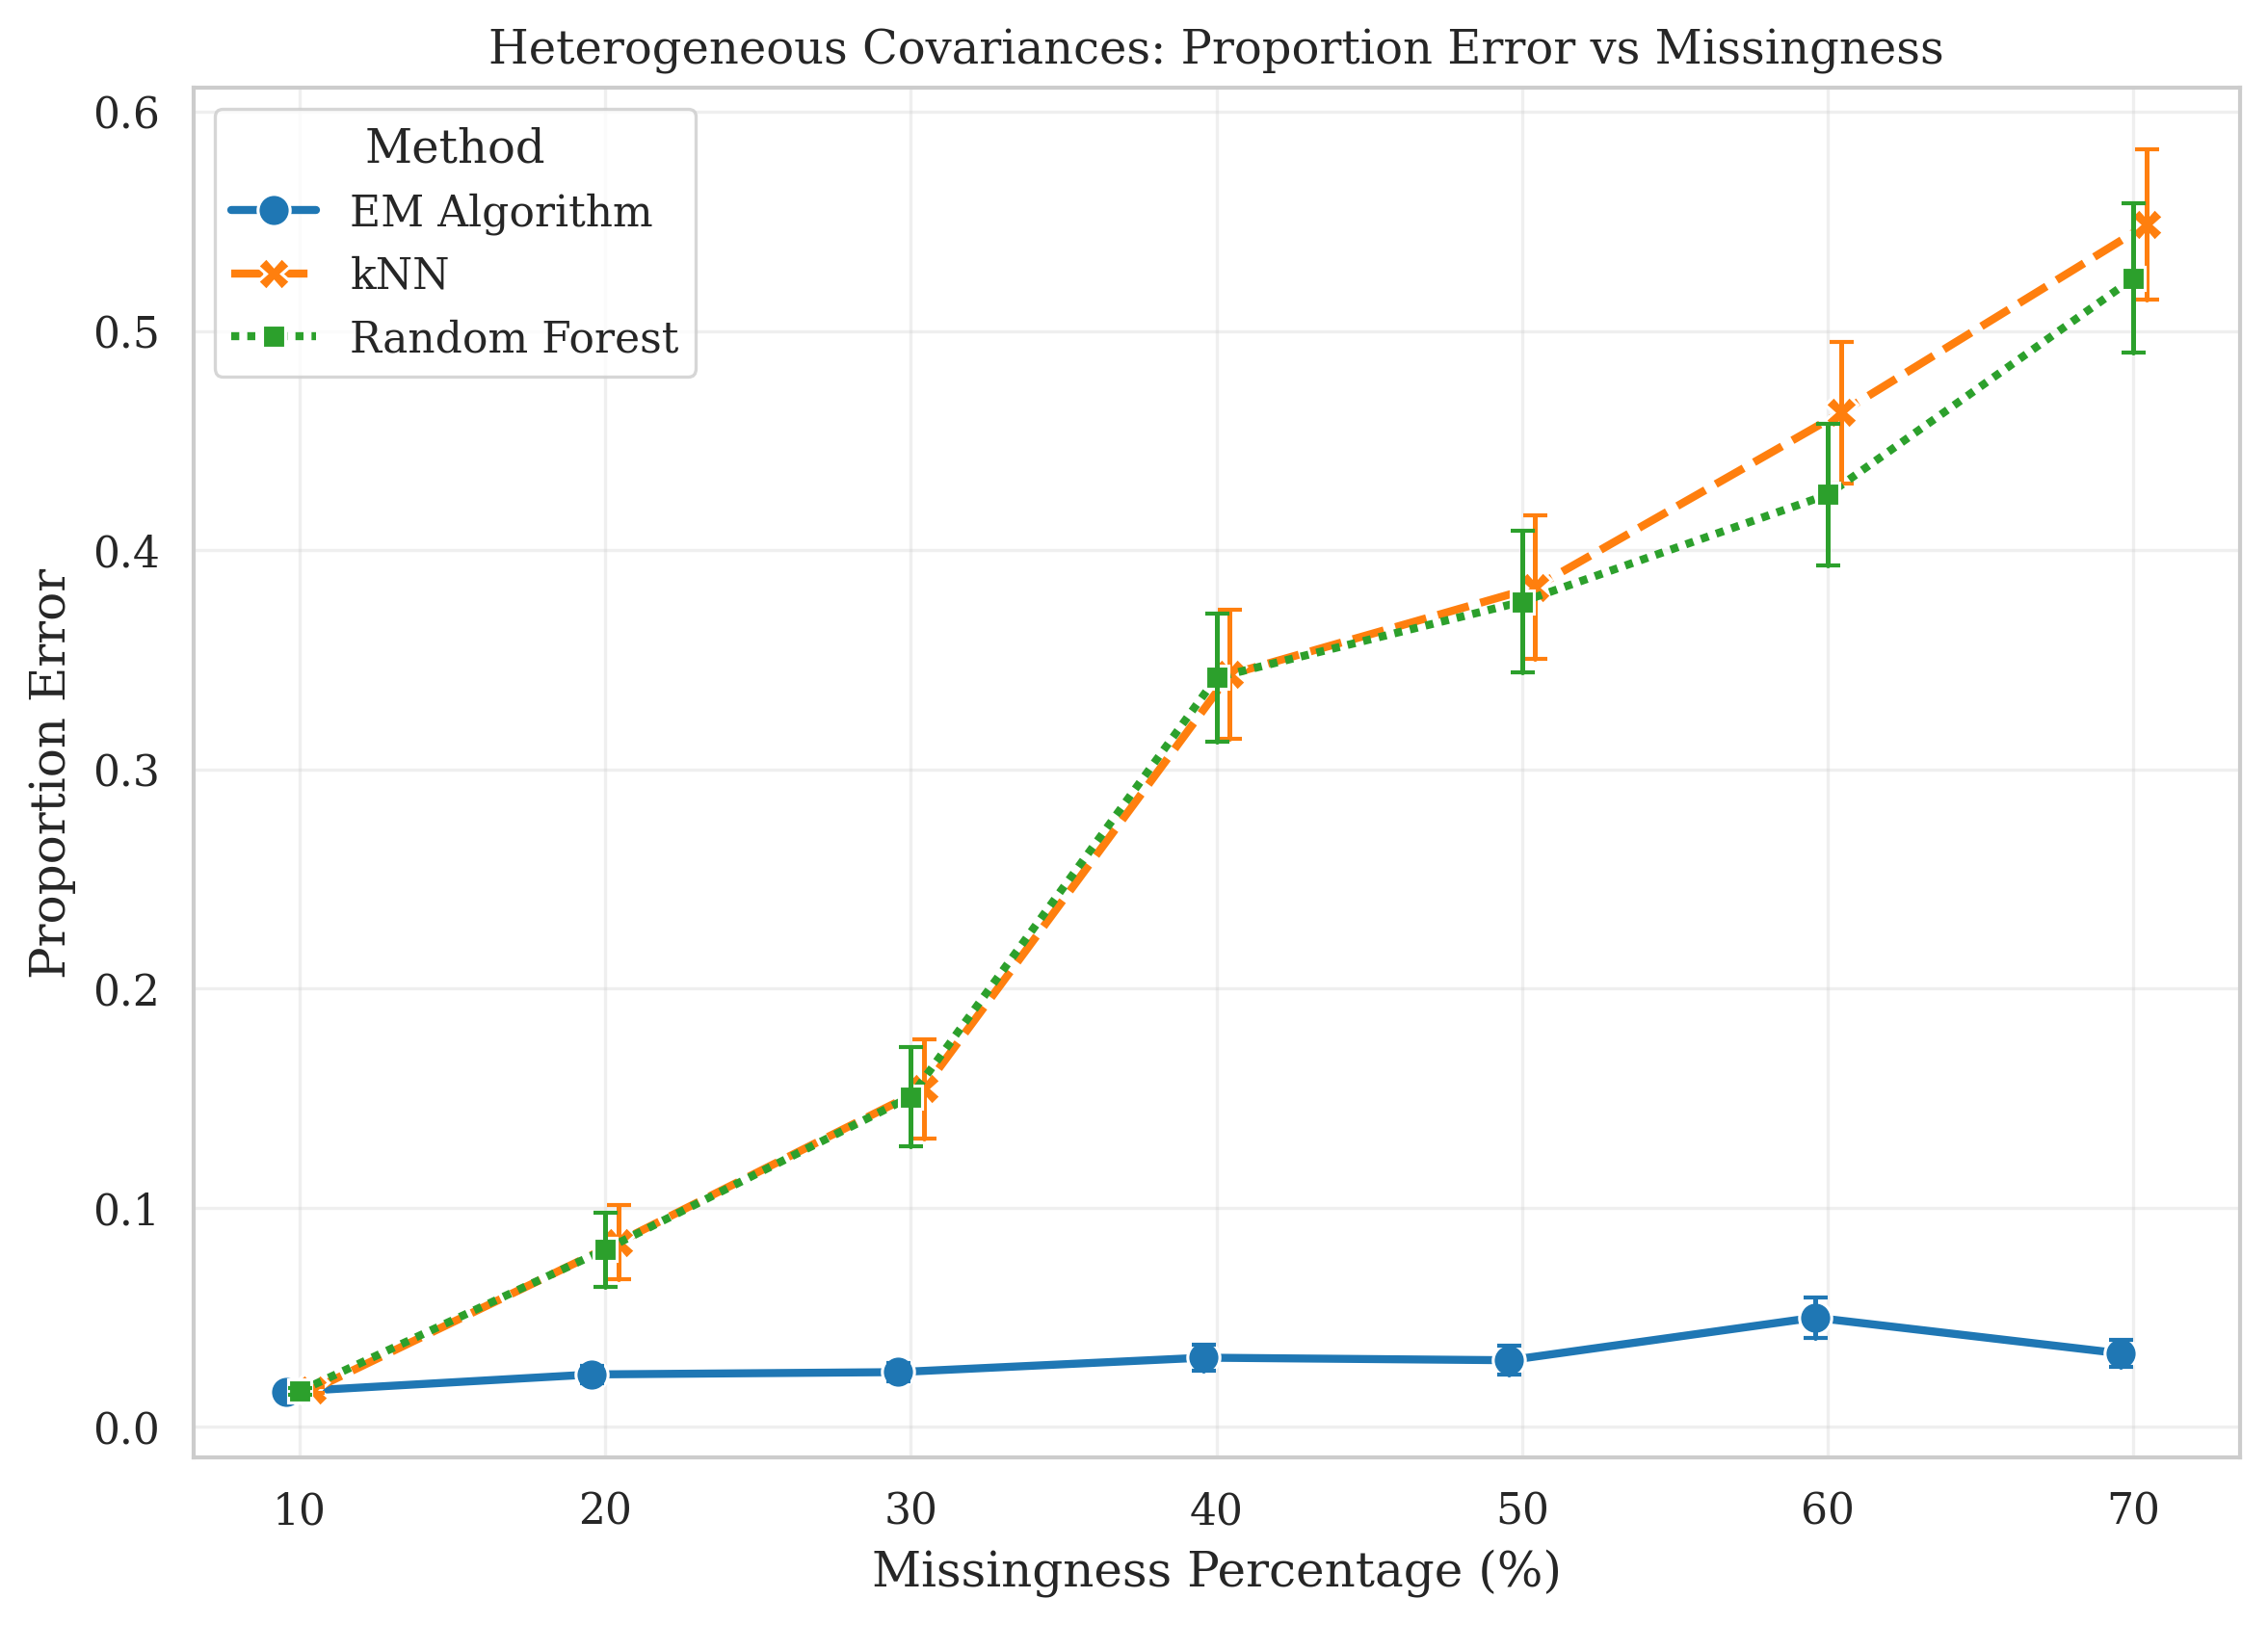
\includegraphics[width=\textwidth]{plots/additional_visualizations/gmm_clustering_scenarios/GMM_Hetero_Cov.png}
        \caption{\textbf{Heterogeneous Covariances}}
    \end{subfigure}
    \caption{\textbf{Structural Analysis of Missing Labels.} Comparison of Proportion Error ($E_{\pi}$) across four geometric configurations. The EM algorithm (Blue) demonstrates superior stability across all scenarios, whereas imputation methods (Green/Orange) exhibit linear degradation, particularly in the High Separation and Heterogeneous cases.}
    \label{fig:gmm_combined}
\end{figure}

As shown in Figure \ref{fig:gmm_combined}, the degradation pattern is consistent across all topologies:

\begin{itemize}
    \item \textbf{Superiority in Latent Structure Recovery:} EM successfully leverages unlabeled data to infer global density, maintaining stability ($E_{\pi} \approx 0.05$) across all geometric scenarios (Panels a, b, d) even at 70\% missingness. In contrast, supervised methods (Random Forest, kNN) suffer a structural breakdown ($E_{\pi} \approx 0.60$), proving them incapable of recovering latent clusters under severe label scarcity.

    \item \textbf{Robustness in Imbalanced Settings:} In the \textbf{Imbalanced Weights} scenario (Panel c), all methods perform effectively due to the prevalence of the dominant class ($E_{\pi} < 0.017$). However, EM demonstrates superior theoretical properties by maintaining a perfectly flat error profile, whereas kNN and Random Forest show slight sensitivity to missingness, albeit with negligible practical impact.
\end{itemize}

\subsubsection{Computational Efficiency}
Finally, we analyze the computational cost of the methods.

\textit{Note on Aggregation: The execution times reported in Figure \ref{fig:gmm_time} are averaged across all simulation runs to isolate the effect of sample size $N$.}

\begin{figure}[h!]
    \centering
    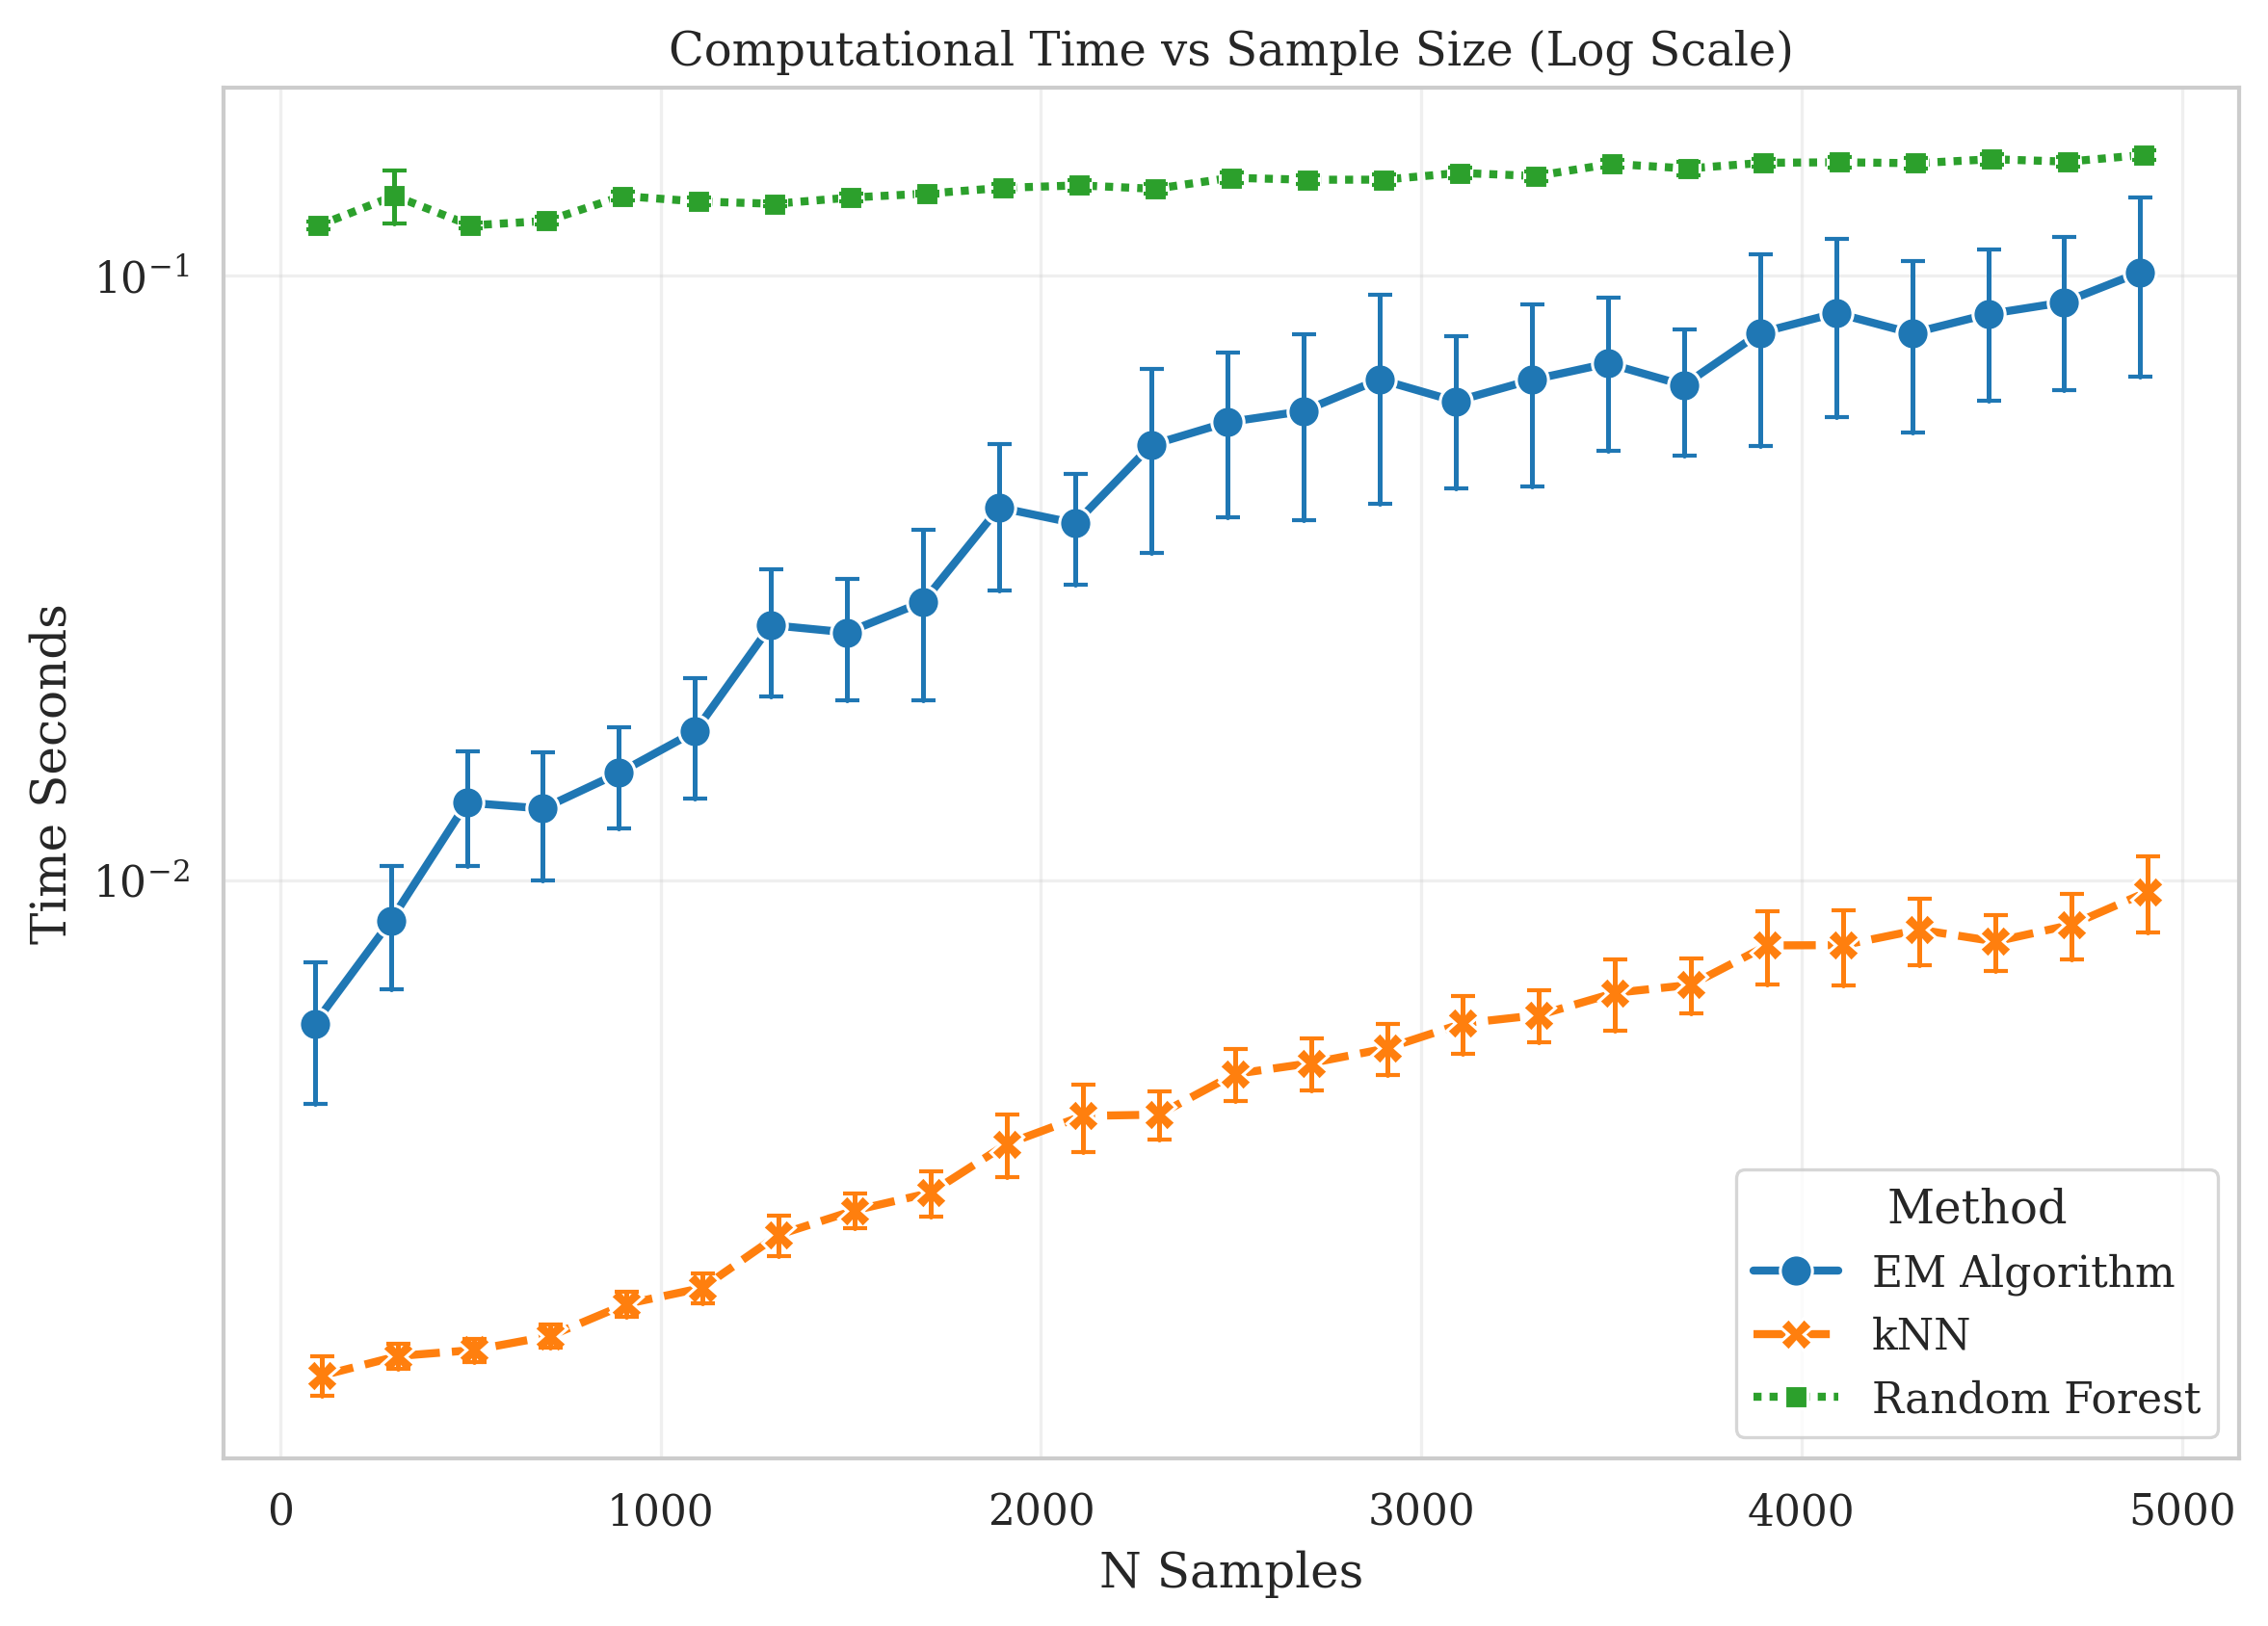
\includegraphics[width=0.7\textwidth]{plots/additional_visualizations/gmm_clustering_scenarios/GMM_Time.png}
    \caption{\textbf{Execution Time vs. Sample Size (GMM).} Note the log scale on the Y-axis. Random Forest (Green) is the slowest, followed by EM (Blue), with kNN (Orange) being the fastest.}
    \label{fig:gmm_time}
\end{figure}

In this context, Random Forest proved to be the most computationally expensive method, likely due to the overhead of training an ensemble on increasing data subsets. The EM algorithm occupies the middle ground; its iterative nature requires repeated passes over the data ($N_{samples} \times N_{iterations}$), but for low-dimensional spaces ($p=5$), it  still remains efficient ($\approx 0.1s$ for $N=5000$).

% --- SECTION 5: REAL DATA APPLICATION ---
\subsection{Real Data Validation}

We applied the semi-supervised framework to the Gastrointestinal Lesions dataset described in Section 3.6. The goal was to verify if the trade-off between dimensionality and sample size observed in the simulations holds for real medical data.

\subsubsection{Results Analysis}
The performance of the imputation strategies for both high ($p=10$) and low ($p=3$) dimensional spaces is summarized in Table \ref{tab:real_data_results}.

\begin{table}[h!]
    \centering
    \small
    \caption{\textbf{Performance on Gastrointestinal Lesions ($N=76$).} Comparison of Accuracy and Class-Specific Recall.}
    \label{tab:real_data_results}
    \begin{tabular}{lcccccc}
        \toprule
        \multirow{2.5}{*}{\textbf{Method}} & \multicolumn{3}{c}{\textbf{10 Dimensions}} & \multicolumn{3}{c}{\textbf{3 Dimensions}} \\
        \cmidrule(lr){2-4} \cmidrule(lr){5-7}
         & \textbf{Accuracy} & \textbf{Recall (Hyp.)} & \textbf{$\Delta \pi$ Error} & \textbf{Accuracy} & \textbf{Recall (Hyp.)} & \textbf{$\Delta \pi$ Error} \\
        \midrule
        Mode Imputer & 0.763 & 0.286 & 0.072 & 0.763 & 0.286 & 0.072 \\
        \textbf{KNN Imputer} & \textbf{0.882} & \textbf{0.762} & \textbf{0.013} & \textbf{0.803} & 0.476 & 0.092 \\
        Random Forest & 0.816 & 0.524 & 0.079 & 0.737 & 0.381 & 0.079 \\
        \textbf{EM Algorithm} & 0.763 & 0.286 & 0.158 & 0.750 & \textbf{0.619} & \textbf{0.017} \\
        \bottomrule
    \end{tabular}
\end{table}

\paragraph{Scenario A: High Dimensionality ($p=10$).}
In the 10-dimensional setting, the \textbf{KNN Imputer} achieved the best performance (Accuracy $0.88$, Recall Class 0 $\approx 0.76$). The \textbf{EM algorithm} failed to converge to a meaningful solution, yielding results identical to the naive Mode Imputer (Recall Class 0 $\approx 0.29$).
This aligns with our simulation results: with $N=76$ and $p=10$, the ratio of samples to parameters is insufficient for the EM algorithm to reliably estimate the $10 \times 10$ covariance matrices (requiring the estimation of 55 parameters per cluster), leading to a degenerate solution.

\paragraph{Scenario B: Low Dimensionality ($p=3$).}
When the dimensionality is reduced to $p=3$, the behavior of the \textbf{EM algorithm} changes drastically:
\begin{itemize}
    \item \textbf{Parameter Recovery:} EM achieves the lowest estimation bias for the class priors ($\Delta \pi = 0.017$), significantly outperforming KNN ($\Delta \pi = 0.092$).
    \item \textbf{Minority Class Recovery:} The recall for the minority class (Hyperplastic) using EM jumps to $61.9\%$, whereas the supervised methods (RF, KNN) struggle to identify these rare instances in the compressed feature space.
\end{itemize}

\subsubsection{Conclusion on Real Data}
The real-world application confirms the central thesis of this study. \textbf{KNN} is robust and preferable in high-dimensional, small-sample regimes ($N \approx p^2$) where density estimation is ill-posed. However, when the dimensionality is low enough to satisfy the structural assumptions ($N \gg p$), the \textbf{EM algorithm} offers superior parameter recovery and deals more effectively with the probabilistic uncertainty of the missing labels.
% --- SECTION 5: DISCUSSION AND CONCLUSION ---

\section{Discussion and Conclusion}

This study provided a comprehensive evaluation of likelihood-based (EM) and imputation-based (MICE, kNN, Random Forest) strategies for handling missing data, combining controlled synthetic simulations with a real-world medical application.

Our analysis in the multivariate normal setting revealed that the covariance structure is the primary determinant of algorithmic performance. The EM algorithm proved to be the optimal choice when variables are highly correlated ($\rho \geq 0.9$), effectively leveraging the observed information in one variable to recover missing values in another. In these high-correlation settings, EM significantly outperformed univariate imputation methods and matched or surpassed MICE. Conversely, in scenarios of independence or weak correlation, the computational overhead of EM yielded marginal gains, making simple heuristics or univariate imputation sufficient and more efficient.

In the context of semi-supervised clustering, the advantage of likelihood-based methods became even more pronounced. By treating missing labels as latent variables, the EM algorithm utilized the distributional information of unlabeled data to stabilize parameter estimates. This contrast was stark against supervised methods like Random Forest and kNN, which, by discarding unlabeled instances, collapsed under conditions of label scarcity, leading to substantial estimation errors even in geometrically simple scenarios. This finding underscores that when the structural assumptions of the model align with the data, model-based approaches maximize information usage in ways that heuristic imputation cannot.

Crucially, however, the application to the gastrointestinal lesions dataset highlighted a fundamental trade-off between model complexity and sample size. While EM dominated in low-dimensional synthetic settings, it exhibited fragility in high-dimensional, small-sample regimes ($N=76, p=10$). In this specific context, kNN Imputation emerged as the most robust strategy, offering superior accuracy by relying on local similarity rather than ill-posed global density estimation. The EM algorithm regained its superiority only after dimensionality reduction ($p=3$), confirming that likelihood-based inference requires a sufficient sample-to-parameter ratio to be effective.

Finally, our asymptotic analysis confirmed the persistent challenge of Missing Not at Random (MNAR) mechanisms. Across all scenarios, increasing the sample size did not mitigate the estimation bias, demonstrating that without explicit modeling of the missingness mechanism, neither likelihood maximization nor heuristic imputation can recover the true parameters.

In light of these findings, we suggest that researchers prioritize likelihood-based methods like EM for low-dimensional or highly correlated datasets, particularly in semi-supervised settings with few labels. Conversely, non-parametric approaches such as kNN or Random Forest are recommended for high-dimensional datasets with limited samples, where the flexibility of local approximation outweighs the theoretical optimality of parametric models.

% --- Section 7: References ---

\renewcommand{\refname}{} % This hides the automatic BibTeX heading
\section{References}      % This keeps your numbered heading "7. References"
\vspace{-3em}             % Removes the whitespace left by the hidden heading
\bibliography{references}

\newpage
\appendix
\section{Appendix}

\subsection{Additional Computational Efficiency Plots}
In Section 4.1.4, we analyzed the computational time for the MAR mechanism. For completeness, we provide here the execution time analysis for MCAR and MNAR mechanisms. As observed in Figure \ref{fig:time_appendix}, the trends are consistent with the MAR case reported in the main text: kNN exhibits quadratic growth with sample size, while the EM algorithm scales linearly but with a higher intercept due to the iterative nature of the likelihood maximization.

\begin{figure}[h!]
    \centering
    \begin{subfigure}[b]{0.48\textwidth}
        \centering
        % Assicurati che questi file esistano o rimuovi la figura se non li hai generati
        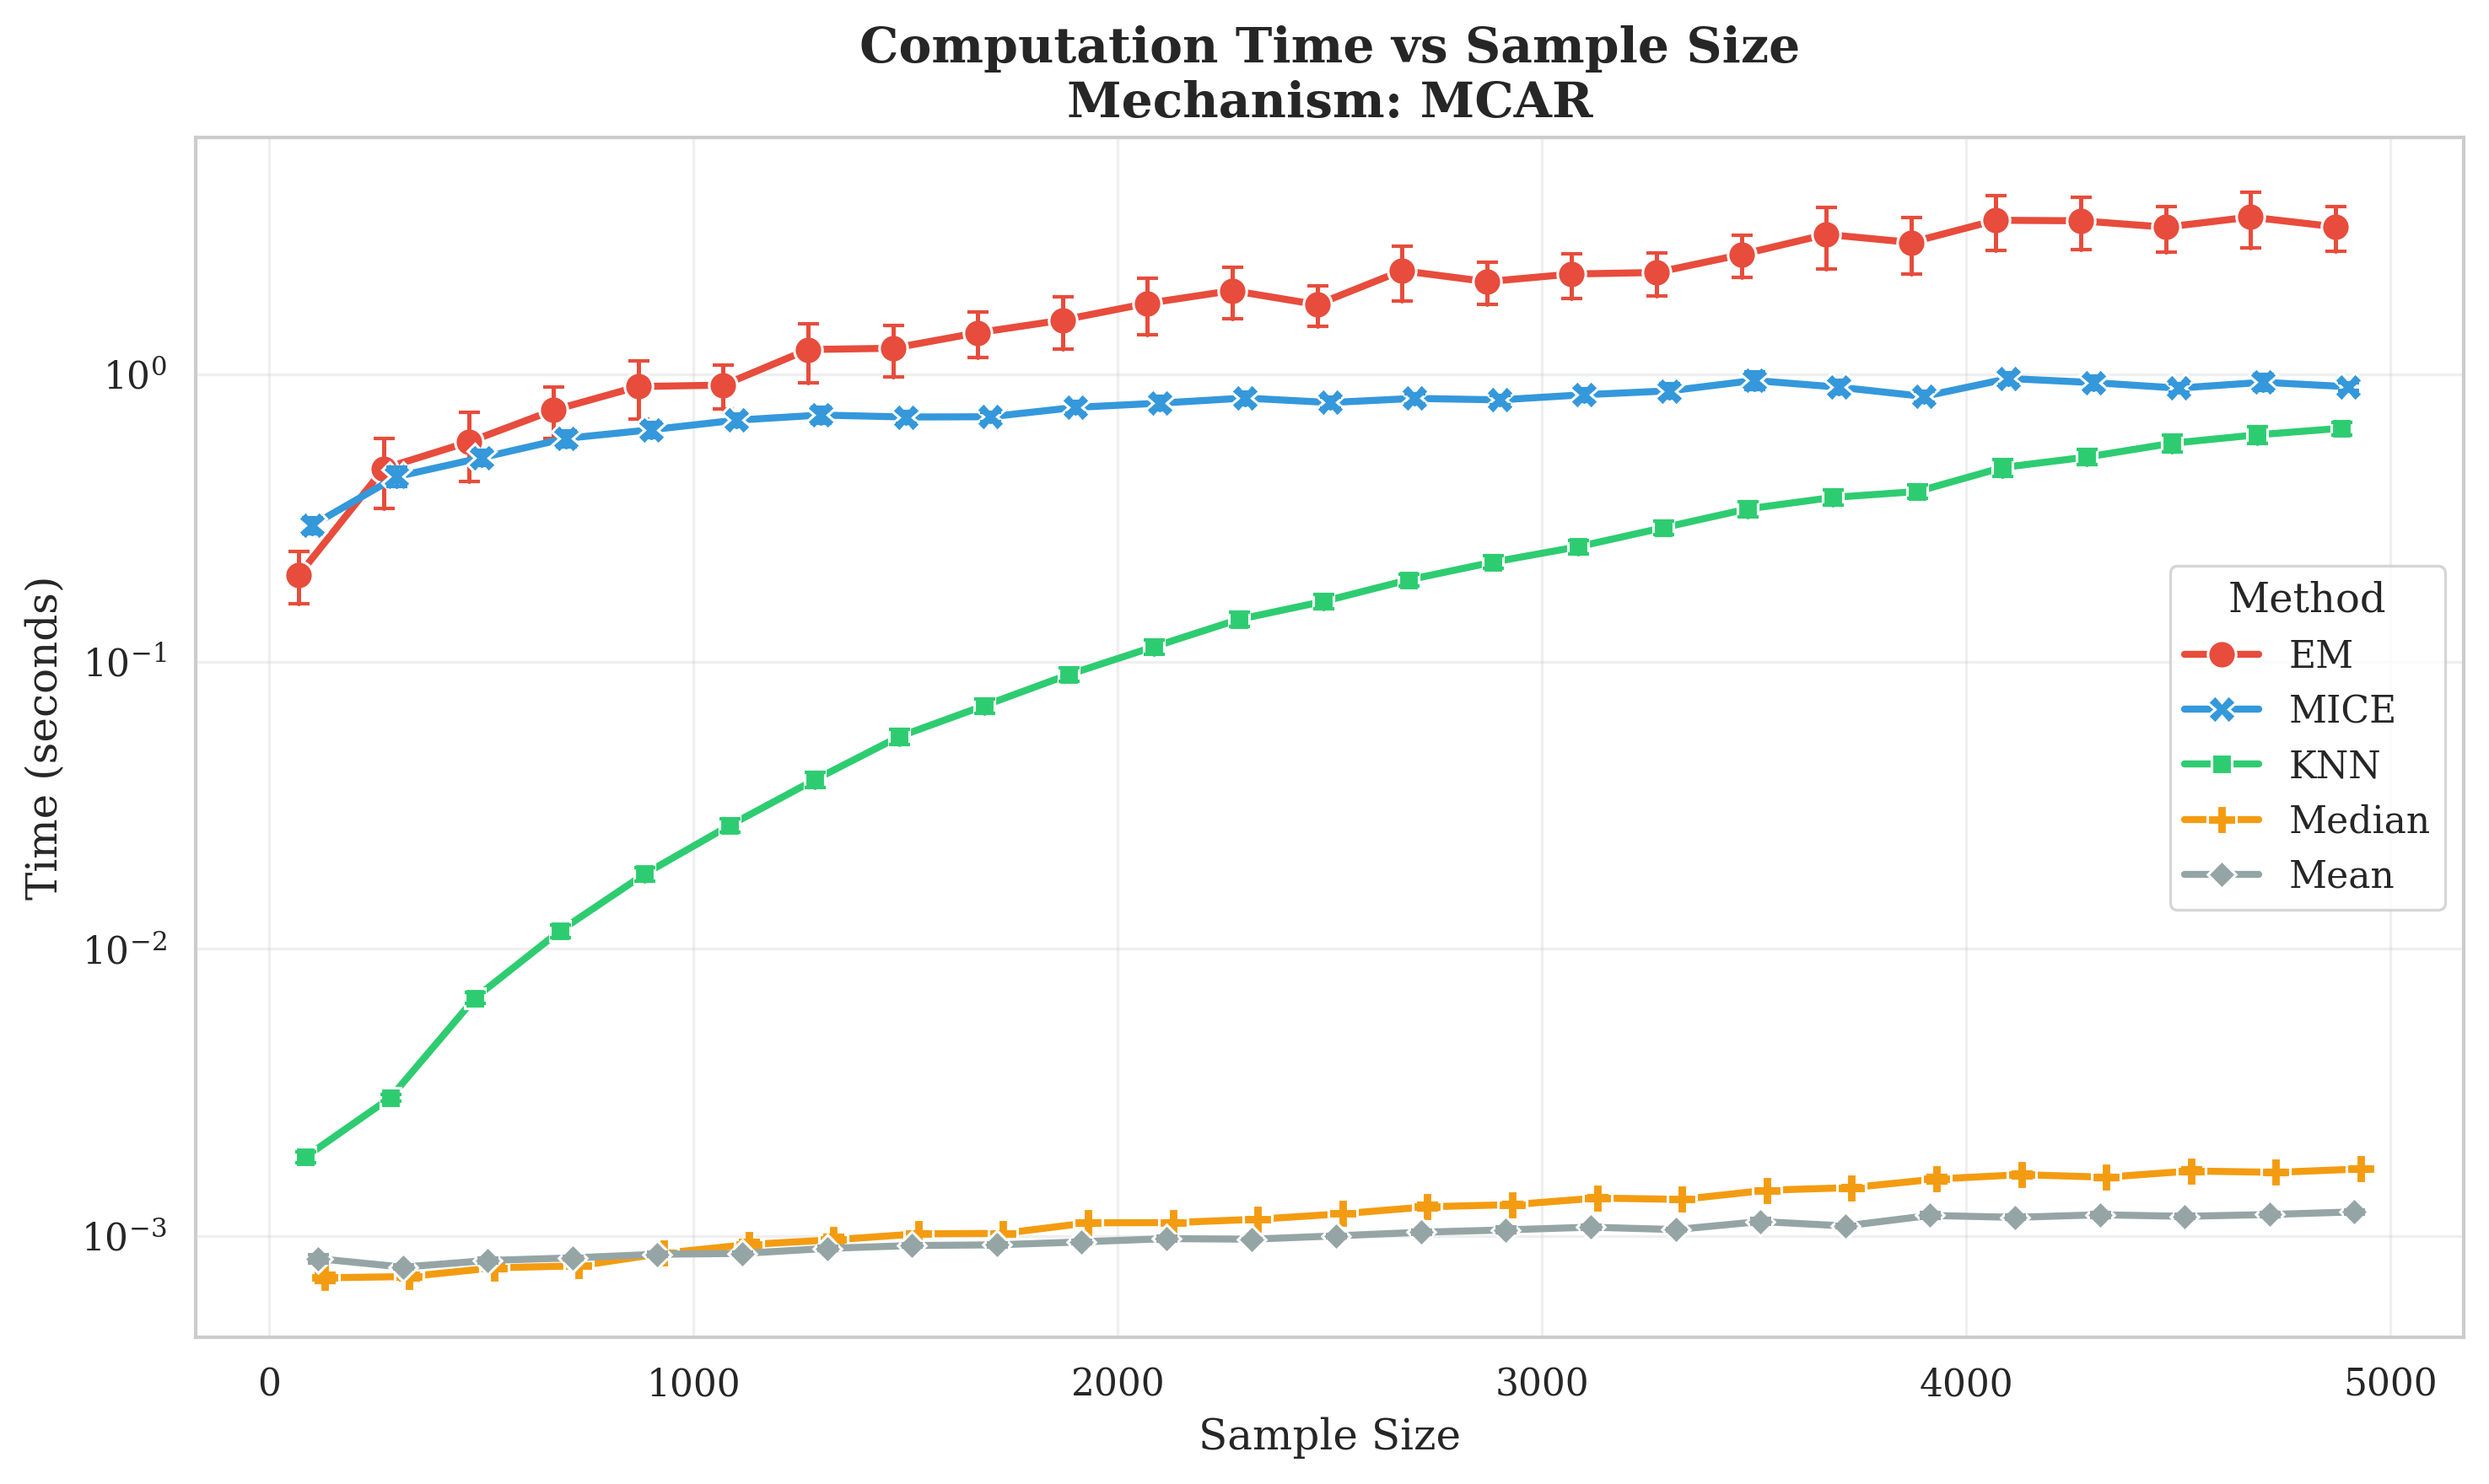
\includegraphics[width=\textwidth]{plots/synthetic_multivariate/MCAR/sample_size_time_MCAR.png} 
        \caption{\textbf{MCAR Mechanism}}
    \end{subfigure}
    \hfill
    \begin{subfigure}[b]{0.48\textwidth}
        \centering
        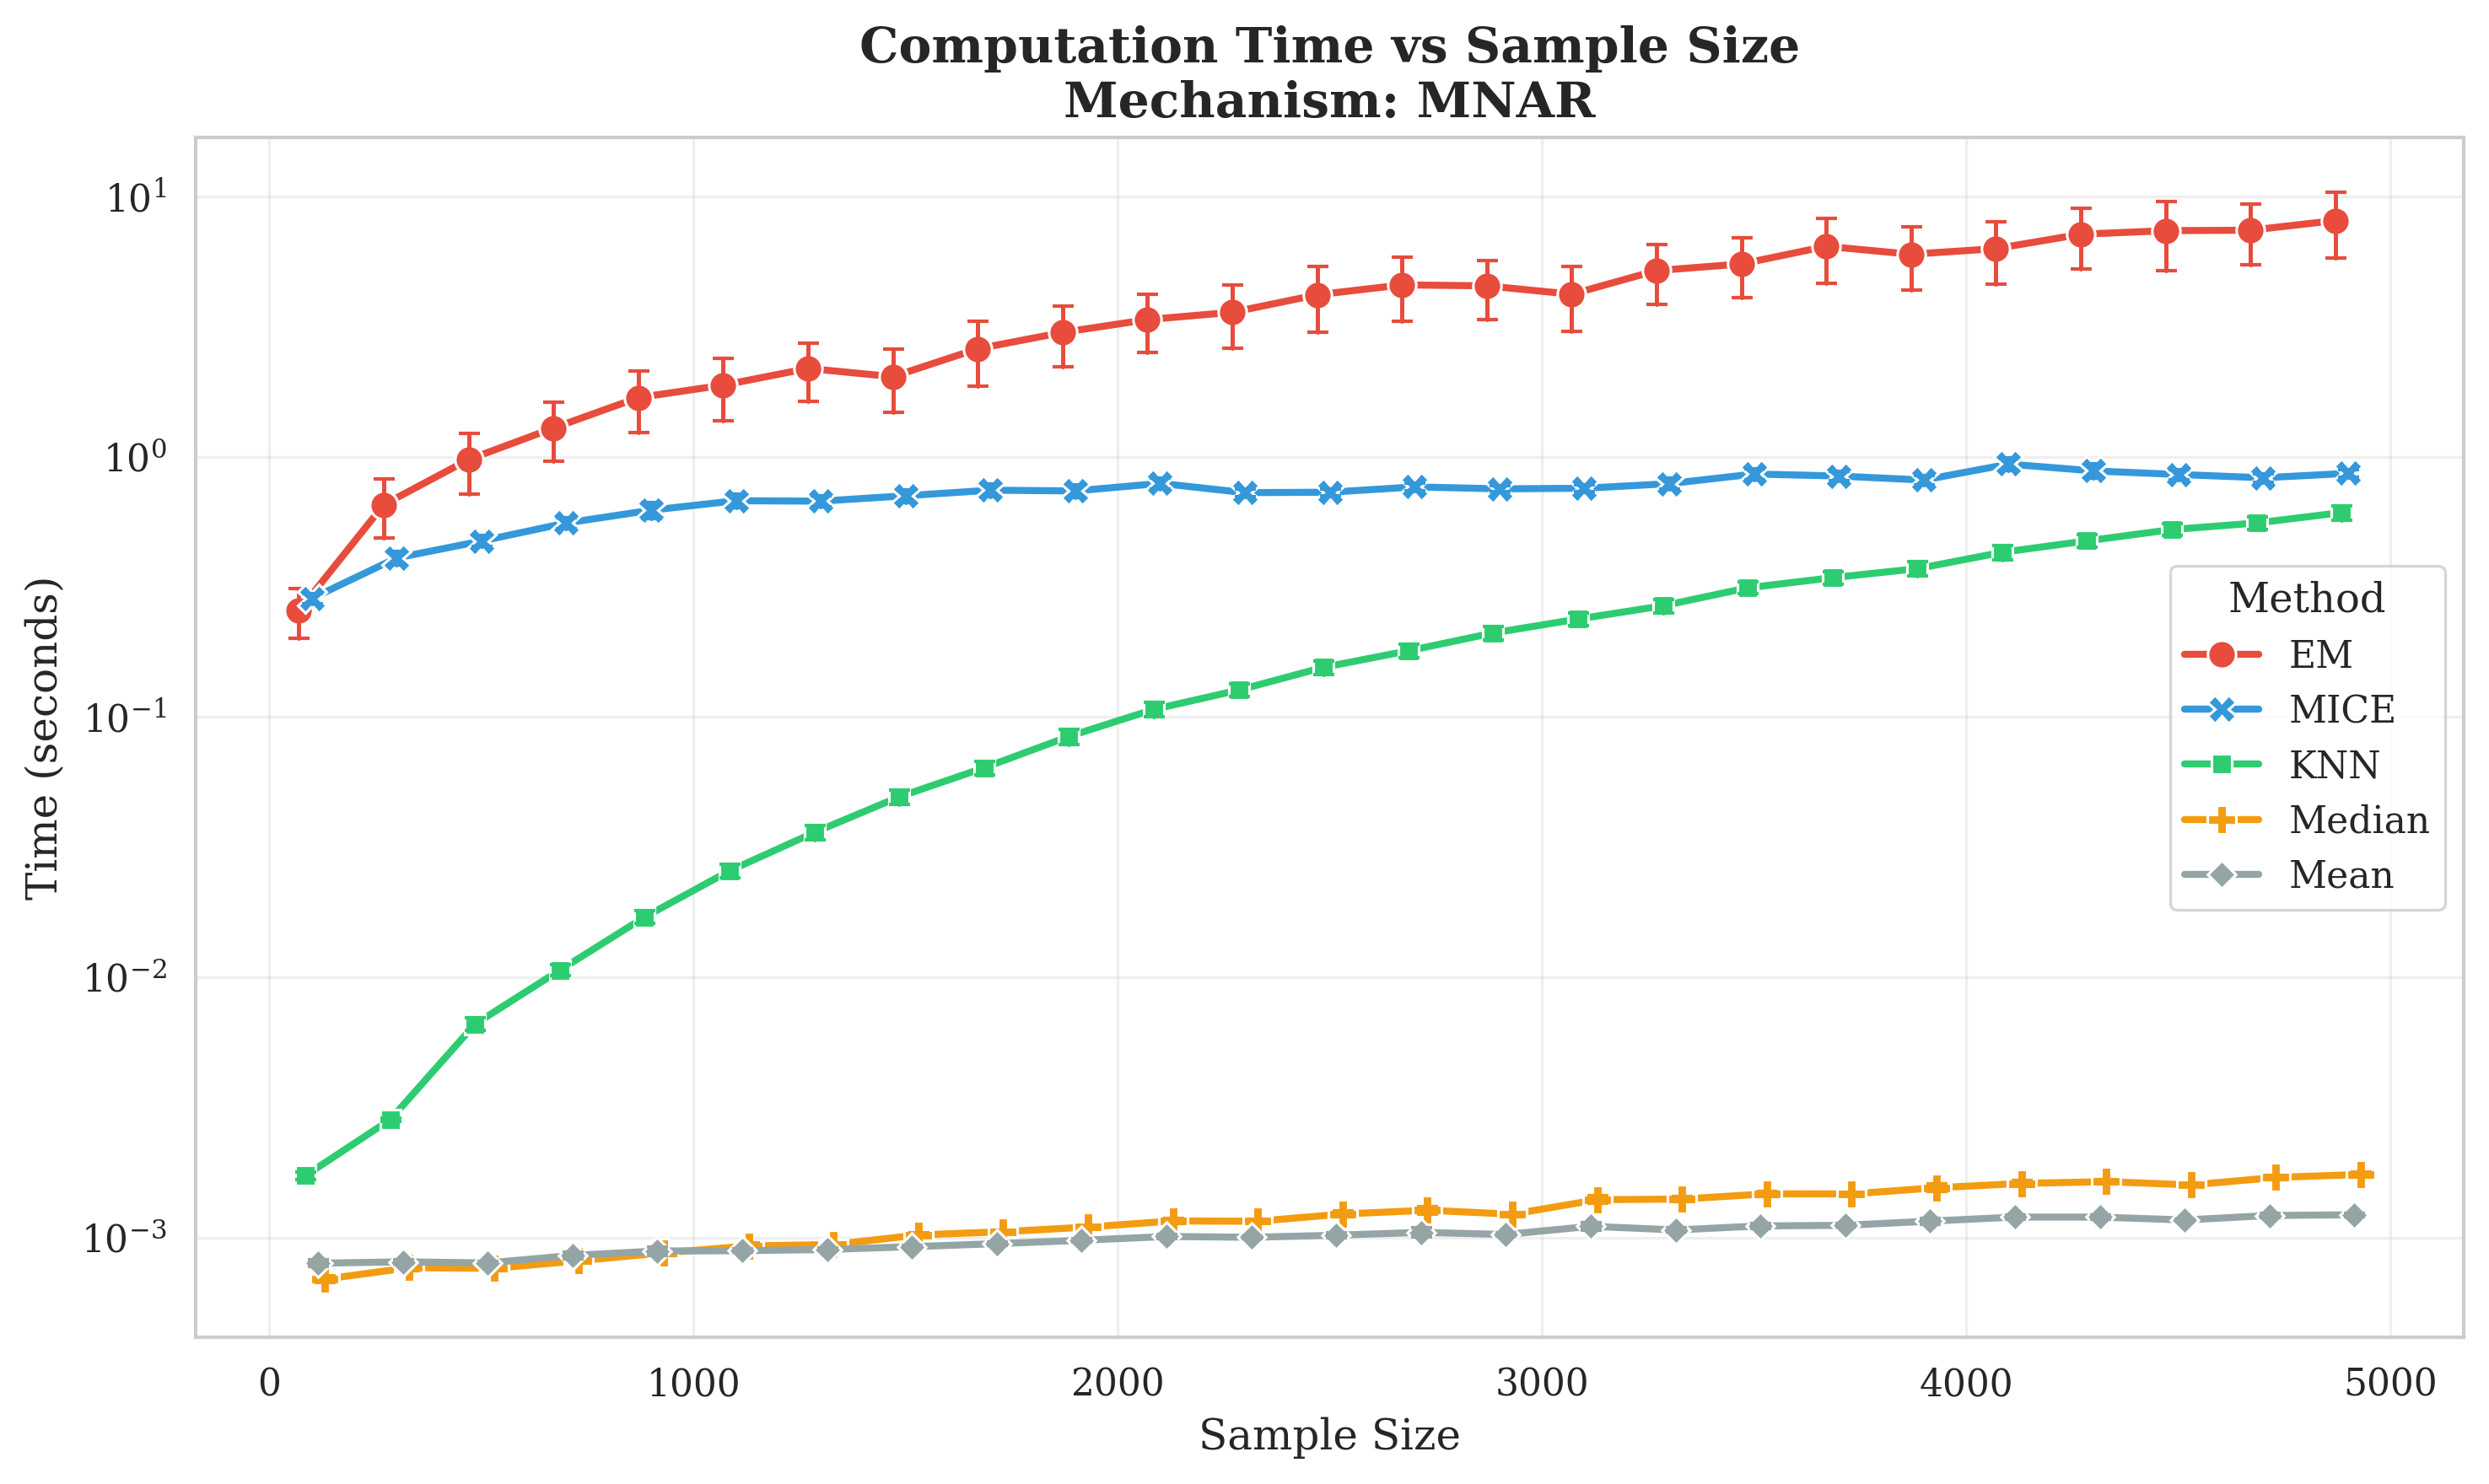
\includegraphics[width=\textwidth]{plots/synthetic_multivariate/MNAR/sample_size_time_MNAR.png}
        \caption{\textbf{MNAR Mechanism}}
    \end{subfigure}
    \caption{Computational Time vs. Sample Size (Log Scale) for MCAR and MNAR mechanisms.}
    \label{fig:time_appendix}
\end{figure}

\subsection{Code Availability}
All simulations, including the data generation processes for MVN and GMM, the implementation of the EM algorithm, and the evaluation scripts, are available in the accompanying code repository. The implementation relies on standard Python libraries (\texttt{numpy}, \texttt{scikit-learn}, \texttt{scipy}) to ensure reproducibility and facilitate further research.

\end{document}



